\documentclass[phd,electronic,oneside,letterpaper,chaptercenter,parttop,lof]{byumsphd}
\usepackage[
    bookmarks=true,
    bookmarksnumbered=true,
    breaklinks=false,
    raiselinks=true,
    pdfborder={0 0 0},
    colorlinks=false,
    plainpages=false,
    ]{hyperref}
    
% This makes hyperlinks point to the tops of figures, not their captions
\usepackage[all]{hypcap}

% These packages allow the bibliography to be sorted alphabetically and allow references to more than one paper to be sorted and compressed (i.e. instead of [5,2,4,6] you get [2,4-6])
\usepackage[numbers,sort&compress]{natbib}
%Commented out by Jie
%\usepackage{hypernat}
%Add by Jie
\usepackage{graphicx}
\graphicspath{{../fig/}}
\DeclareGraphicsExtensions{.pdf,.jpeg,.png,.jpg}
\usepackage{caption}
\usepackage{subcaption}
%\usepackage{makeidx}
%\makeindex

% Because I use these things in more than one place, I created new commands for
% them.  I did not use \providecommand because I absolutely want LaTeX to error
% out if these already exist.
\newcommand{\Title}{Animating Non-rigid Bodies using Motion Capture}
\newcommand{\Author}{Jie Long}
\newcommand{\GraduationMonth}{January}
\newcommand{\GraduationYear}{2013}

% Set up the internal PDF information so that it becomes part of the document
% metadata.  The pdfinfo command will display this.
\hypersetup{%
    pdftitle=\Title,%
    pdfauthor=\Author,%
    pdfsubject={PhD Dissertation, BYU CS Department: %
                Degree Granted \GraduationMonth~\GraduationYear, Document Created \today},%
    pdfkeywords={Motion capture, non-rigid bodies, plant modeling, wind dynamics, particle flow},%
}

% Rewrite the itemize, description, and enumerate environments to have more
% reasonable spacing:
\newcommand{\ItemSep}{\itemsep 0pt}
\let\oldenum=\enumerate
\renewcommand{\enumerate}{\oldenum \ItemSep}
\let\olditem=\itemize
\renewcommand{\itemize}{\olditem \ItemSep}
\let\olddesc=\description
\renewcommand{\description}{\olddesc \ItemSep}

% Important settings for the byumsphd class.
\title{\Title}
\author{\Author}

\committeechair{Michael~Jones}
\committeemembera{Parris~Egbert}
\committeememberb{Bryan~Morse}
\committeememberc{Eric~Mercer}
\committeememberd{Sean~Warnick}

\monthgraduated{\GraduationMonth}
\yeargraduated{\GraduationYear}
\yearcopyrighted{\GraduationYear}

\documentabstract{
When working with a complex AI or robotics system in a specific application, users often need to incorporate their special domain knowledge into the autonomous system. Such needs call for the ability to \textit{manage autonomy}. However, managing autonomy can be a difficult task because the internal mechanisms and algorithms of the autonomous components may be beyond the users' understanding. We propose an approach where users manage autonomy indirectly by \textit{managing information} provided to the intelligent system at three different scales: Strategic, Between-Episodes, and Within-Episode. Information management tools at multiple scales allow users to influence the autonomous behaviors of the system without the need for tedious direct/manual control. 



However, to make these tools truly effective, users need to clearly see and understand the causal relationships between information change and autonomous behavior change. Information fed to the system can be in the forms of ``user-friendly'' model parameters, datasets, areas of focus, representations of task difficulty, and the amount of autonomy desired. We apply this approach to using an Unmanned Aerial Vehicle (UAV) to support Wilderness Search and Rescue (WiSAR), and show that this approach improves the experience of the human partner in human-robot interaction and the performance of the human-robot team.

}

\documentkeywords{%
    Motion capture, non-rigid bodies, plant modeling, wind dynamics, particle flow
}

\acknowledgments{
I would like to express my deepest gratitude to my advisor, Dr.\ Michael A. Goodrich for his continuous guidance and support throughout the research, for his encouragement, patience, trust in me, and for making this a thoughtful and rewarding journey. He sets an excellent example of a dedicated scientist. His thoughtful insights, both in scientific research and in living everyday life, have always helped me overcome one after another challenges. I am very grateful to have such a wonderful mentor, colleague, and good friend for life. I want to extend my appreciation to the rest of my dissertation committee: Dr.\ Bryan Morse, Dr.\ Mark Colton, Dr.\ Kevin Seppi, and Dr.\ David Embley for their support over the years as I grew from a clueless grad school student to a confident researcher.

I want to thank all those (lab mates, colleagues, reviewers, and etc.) who helped me with my research, whether it was a brainstorming idea, collaborative work, or critiques, for helping me grow intellectually. I would also like to thank the BYU Computer Science Department for providing an encouraging and inspiring research environment, so I can turn my passion about Artificial Intelligence and Robotics since childhood into a constructive career.

Last but not least, I would like to thank my wife, Noelle, for her patience/impatience and encouragement/discouragement during the journey, and my children, Adeline and Isaac, for their beautiful smiles, which inspire me to better myself day after day.
}

\department{Computer~Science}
\graduatecoordinator{Dan~Ventura}
\collegedean{Thomas~W.~Sederberg}
\collegedeantitle{Associate~Dean}

% Customize the name of the Table of Contents section.
\renewcommand\contentsname{Table of Contents}

% Remove all widows an orphans.  This is not normally recommended, but in a
% paper dissertation there is no reasonable way around it; you can't exactly
% rewrite already-published content to fix the problem.
\clubpenalty 10000
\widowpenalty 10000

% Allow pages to have extra blank space at the bottom in order to accommodate
% removal of widows and orphans.
\raggedbottom

% Produce nicely formatted paragraphs. There is nothing additional to do.  In
% case you get some problems, surround your text with
% \begin{sloppy} ... \end{sloppy}. If that does not work, try
% \microtypesetup{protrusion=false} ... \microtypesetup{protrusion=true}
\usepackage{microtype}

\begin{document}

% Produce the preamble
\microtypesetup{protrusion=false}
\maketitle
\microtypesetup{protrusion=true}

\chapter{Background, Motivation, and Overview}
Simulating non-rigid bodies with data from motion capture is a new application of motion capture. We present a motion reconstruction approach for non-rigid bodies in the context of motion capture.  Passive optical motion capture records movements of non-rigid bodies by tracking locations of retroreflective sensors placed on subjects. By processing the recorded motion data and combining the data with physical and statistical models, we create complete animation of non-rigid bodies. We focus on animating natural trees and ropes as instances of non-rigid bodies.  Motion is captured in the presence of external forces, such as wind and human interaction. 

Rope is one of the simplest non-rigid bodies. Animating ropes is a simple platform from which to evaluate the motion capture process, including data collection and processing. The capture process then can be generalized and applied to other non-rigid subjects, such as natural trees. We present methods that can be used to create natural tree motion in wind using physical and statistical models. The resulting motion is visually plausible and scalable. 

Animating non-rigid bodies has important applications in computer-generated movies, video games, and forestry engineering. In movie and video games where computational resources are a concern, directors need a simple process to use the motion of non-rigid bodies as part of telling a story. Motion capture hardware has been popular in movie and game production for many years.  Motion capture equipment is easy to set up and provides motion data with good accuracy in both time and space.  The hardware integrates camera calibration algorithms and greatly simplifies the process of recording position information in real-world 3D space. Many movies use motion capture to record motion from real characters and then drive virtual characters with the collected motion data \cite{Jesser2010}. Motion capture produces realistic motion data while reducing the cost for creating motion in different environments or in fictional environments. 

The equipment has flexibility for capturing both rigid bodies and non-rigid bodies. However, most research and applications focus on rigid bodies. As a non-rigid body, a tree has motion that is important in film and games because trees swaying in the wind can set the mood or feel for a scene, so directors can use tree motion as a tool for telling stories. In the field of forestry, our research helps forestry engineers understand the influence of wind on trees. This can inform decisions for pruning trees or protecting structures. Rope, the other application explored in this work, has simple structure and dynamics. But when the motion of a human character interacting with the rope is captured in the same scene, the replay of both rope and human motion becomes difficult. Movie makers may be able to use our motion capture process and create animation with interactions between rigid and non-rigid bodies.

Human motion capture using a rigid body model, such as \cite{Lou:EHM2010,Wen:2006:MCD,Rajko:2007:RAK,ZordanVictorBrian2003}, is a well-studied area in motion capture but is less applicable to our research, as removing the rigid body assumption changes the problem. There are two common approaches to extracting human motion from motion capture data. One is to extract a skeleton model or kinematic model from motion data \cite{Lou:EHM2010,Rajko:2007:RAK}. The other is to predefine the skeleton and to apply motion capture-data to animate the predefined skeleton \cite{Wen:2006:MCD,ZordanVictorBrian2003}. Most of the methods have an important assumption that the distance between any pair of markers is non-changeable. However, this assumption does not stand for non-rigid bodies, which is the essential difference for motion capture of rigid bodies and non-rigid bodies. Instead of a skeleton of rigid parts, non-rigid motion capture focuses on reconstructing a mesh that deforms to match a moving surface such as a face or cloth. We investigate non-rigid motion capture but we focus on curved splines rather than curved surfaces.

Motion capture of non-rigid bodies is difficult. Prior work on non-rigid motion capture is mainly focused on facial motion \cite{Lorenzo03,SifakisEftychios2005} and cloth motion \cite{MarcusVolker04clothmotion,whiteRyan2007siggraph,PritchardDavid2003,Bhat2003}. Both facial motion and cloth motion aim to represent the motion of a surface. Motion capture of thin, rod-shaped non-rigid bodies such as rope or tree branches is a fundamentally different problem. For instance, rope, as a non-rigid body, is more naturally represented as a curved spline rather than as a curved plane (though a curved spline can be used to drive the motion of a plane). Worring's \cite{WorringMarcel94measurementof} prior work in reconstruction of a line-shaped object in 3D from several computer images builds non-rigid rope motion but would require a foreground-- background separation step and a sharp image of the rope in each frame.

Part of animating trees in wind is modeling the 3D shape of the tree to be animated. Tree shape modeling has long been studied on computer graphics. A tree with natural appearance greatly improves visual quality of tree animation. These methods include particle systems \cite{Reeves83particlesystems,Runions07,palubicki:siggraph09,neubert:acmtg07}, L-systems \cite{lindenmayer68,Lintermann1999,Prusinkiewicz:2001}, parametric models \cite{Weber1995}, photographs \cite{RecheMartinez2004,neubert:acmtg07,Tan:2007:ITM} or videos \cite{Li:2011:MGM,Diener:2006}. Most of these methods result in satisfying tree shapes but do not leverage the 3D positions of motion capture markers, which are recorded as part of a motion capture session but require a different set of inputs. Image- or video-based approaches convert a set of 2D input images into 3D tree models by filling in the missing dimension.  Motion capture systems can record tree shape in 3D with high precision (using similar techniques for converting a set of 2D images to a 3D model). Prior work \cite{Long:MCN2010} in reconstructing tree shape from motion capture data using either exact measurements or markers placed within the crown does not scale and does not apply when leaves occlude the branching structure.

Animation of trees in wind has been discussed for many years \cite{Akagi:cg06,stams:eu97,shinya:eu92}. Prior work in animating 3D tree models focuses on recreating branch motion due to wind turbulence. Wind turbulence has been simulated and has been synthesized from the frequency spectrum of turbulence created by tree crowns. Simulation-based models create tree motion based on the tree's biomechanical characteristics and wind dynamics \cite{Akagi:cg06,Habel09PGT}. Spectral approximation describes tree swaying and wind velocity field using some computer-generated noise. These systems include techniques based on photographs \cite{wu:cas99} or videos \cite{Diener:2006}, and some parameter-based spectral models \cite{Habel09PGT,shinya:eu92}. In most of the previous research, the wind field is created using noise and fluid simulation. While simulation models capture visually important wind--tree effects, such as crown sheltering, they require expensive computations that are not currently feasible in interactive applications such as games. Spectral approximation ignores sheltering effects and requires significant user intervention, but is computationally efficient. Rather than being based on actual captured tree motion, simulation models and spectral approximations are both theoretically based. Motion capture avoids the directability and computation problems of simulated wind fields but may yield data that validates simulation-based models. 

% From Egbert: put a paragraph here that summarize how your approach is different from the other works that has been done.
Our work differs from the previous work by introducing motion capture in simulating non-rigid bodies. It is also the first work to motion capture bendy thin rods and the first to replay motion capture data from a tree. The resulted animations are mostly driven by data instead of pure physical simulation or stochastic process. We describe a complete approach to animating natural trees using motion capture, including data collection, data processing, generating tree shape, and combining statistics and wind dynamics for the animation. The thesis discusses two approaches for tree animation with different motion capture setups, which require different processes and create tree motion with varying scalability. Rope motion is created using a data-driven approach rather than the pure physical model that is common in previous research. The rope project helps us to better understand the motion-recording capability of motion capture for non-rigid bodies. Using motion capture simplifies the process to parameterize a physical model of a rope under specific motion.

\section{Thesis Statement}

A small portion of known movements collected from motion capture can produce complete movements of non-rigid bodies by combining the motion capture data with physical and statistical models. We show that the resulting motion is visually plausible for trees and rope.

\section{Publications}
This dissertation consists of seven papers, two of which are under review.  The work can be divided into three parts: rope motion reconstruction, tree shape reconstruction, and tree motion reconstruction. The remaining chapters contain these papers.  Chapter 2 is a pilot project in which a simplified motion capture process is presented with statistical analysis for replaying natural tree motion where the motion is not scalable. There is no attempt to retarget or extend the captured data. While we were able to replay the tree motion, it requires a series of careful measurements to recreate the exact tree shape, and the motion cannot be transferred to similar shapes or situations. Chapter 3 describes replaying rope motion. The project focuses on processing motion capture data and uses rope's simple structure to validate estimated data against the collected motion data. The process for motion capture data includes identifying and removing noises and labeling markers. This process was used for both tree and rope motion capture. Chapters 4 and 5 begin a different approach to the problem.  Rather than directly replay the original motion on the original structure, in Chapter 4 and 5 we reconstruct the approximate tree shape from the captured motion in preparation for replaying similar motion on a similar structure. Chapter 6 extracts a force field from captured motion that can be used to animate any tree shape.  

In Chapter 2, the pilot project aims to replay natural tree swaying in wind. Retroreflective markers are placed on a small cherry tree. We infer a skeleton from tree motion data and repair the motion data using a rigid body model. The motion data contain gaps and errors for branches that bend. Motion-data repair is critical because trees are not real rigid bodies. These ideas allow the reconstruction of tree motion, including global effects, but without a complex physical model. Instead, it employs a statistical model. This project builds a complete pipeline for motion capture, including equipment set up, data collecting interface, 3D tree model, and motion integration. However, the scalability of this approach is limited and it requires intensive labor to reproduce the exact tree structure. The work requires markers being placed about 10 cm apart on each branch segment. Leaves have to be removed to enlarge the visibility of markers to motion capture cameras. Branches are assumed to be rigid (to some degree) with small bending capability. 

Chapter 3 begins a study of motion capture for rope and takes a closer look at animating non-rigid bodies using a non-rigid model for motion capture. Rope has a simple structure with no branches and simple geometry. The model is a good test bed for evaluating different algorithms for both data processing and motion replaying. In this project, we provide a more general approach for processing motion capture data from passive optical motion capture for non-rigid bodies rather than adapting a rigid body model as in Chapter 2. The data collection and processing process includes labeling markers and identifying and removing noise. We provide clustering, gap repair, and marker swap detection algorithms based on linear interpolation and forward differencing under the assumption that the rope does not stretch. Indexed marker positions are connected with a spline in each frame to approximate the original rope. The model produces visually plausible animations of rope motion from data collected for a person interacting with rope. However, the method fails when the rope experiences large accelerations that result in motion that is not modeled by forward differencing.

Reconstruction of tree shape, as in Chapters 4 and 5, is an important step in replaying motion capture of trees under external forces, which is the goal of the work presented in Chapter 6. A realistic 3D tree model helps researchers estimate and compare computer-generated animation against the original motion. Existing algorithms for generating branching structures for image synthesis in computer graphics are not adapted to the unique data set provided by motion capture. In Chapter 4, we discuss a method for tree shape reconstruction using particle flow on input data obtained from a passive optical motion capture system. Initial branch tip positions are estimated from averaged and smoothed motion capture data. Branch tips, as particles, are also generated within the bounding space defined by a stack of bounding boxes or a convex hull. The particle flow, starting at branch tips within the bounding volume under forces, creates tree branches. The resulting shapes are realistic and similar to the original tree crown shape. Several tunable parameters provide control flexibility over branching shape and arrangement.

In Chapter 5, we combine a procedural method with particle flow to generate a 3D tree shape. Using L-systems for describing tree branches as particles, our method introduces a hemisphere to generate particles, uses a growth level to simulate different ages of branches, and applies a dynamic bounding box to detect local growth area in a tree. This new method enhances the management of tree shapes by easing the control over distributions of branches and leaves. We also demonstrate that the method has potential to simulate phototropism and growth around physical barriers. We evaluate this model by particle flow and the complexity of this method, showing performance competitive with existing methods.

Chapter 6 discusses non-rigid motion capture by extracting external forces from motion capture data and then replaying those forces to create animation. We explore this idea in the context of motion capture of natural trees in wind. Motion of a tree in wind is decomposed into three forces: wind-induced drag, branch elasticity, and damping by the leaves. Given a model of elasticity and damping, the drag force can be isolated and used to estimate wind velocity. The extracted velocity field is extended to a larger volume and enriched with a turbulence model. That wind field can be replayed on a tree model that includes elastic and damping properties to create similar motion.  The work contained in this chapter is the culminating work of this dissertation.

We list all the citations for each chapter in the order in which they appear.

1. Jie Long, Cory Reimschussel, Ontario Britton, Anthony Hall, and Michael Jones. Performance Capture for Natural Tree Motions in the Wind. Motion in Games , MIG, 2010. 

2. Jie Long, Bryce Porter, Michael Jones. Motion Capture of Rope, not yet published.

3. Jie Long and Michael Jones. 3D Tree Modeling using Motion Capture. IEEE The Fourth International Symposium on Plant Growth Modeling, Simulation, Visualization and Application (PMA '12).

An extended version of this paper is requested for submission to the journal Frontiers in Computer Science . 

4. Jie Long and Michael Jones. A Realistic 3D Tree Model based on L-Systems. Report for UNEP Eco-Peace Leadership Center (EPLC), 2008.

5. Jie Long and Michael Jones. Estimating wind flow from tree motion using motion capture data, not yet published.

In addition, the research on motion capture of trees was presented as a short talk in SIGGRAPH 2009, where a short abstract was published.

Jie Long, Cory Reimschussel, Ontario Britton, and Michael Jones. Motion capture for natural tree animation. International Conference on Computer Graphics and Interactive Techniques, SIGGRAPH 2009: Talks. New Orleans, Louisiana, Article No. 77, 2009. 

Data captured as part of this work was used in a study of tortuosity as a metric for evaluating branch motion paths. The citation for that paper is given below but the paper is not included in the dissertation.  

Michael Jones and Jie Long. Tortuosity as a Metric for Evaluating Branch Motion Paths. IEEE The Fourth International Symposium on Plant Growth Modeling, Simulation, Visualization and Application (PMA '12).

\chapter{Motion Capture for a Natural Tree in the Wind} 
\label{chap:pilottree}

\noindent
Jie Long, Cory Reimschussel, Ontario Britton, and Michael Jones. Motion capture for natural tree animation. \emph{International Conference on Computer Graphics and Interactive Techniques, SIGGRAPH 2009: Talks}. New Orleans, Louisiana, Article No. 77, 2009.

\begin{abstract}
Simulating the motion of a tree in the wind is a difficult problem because of the complexity of the tree's geometry and its associated wind dynamics. Physically based animation of trees in the wind is computationally expensive, while noise-based approaches ignore important global effects, such as sheltering. Motion capture may help solve these problems. In this paper, we present new approaches to inferring a skeleton from tree motion data and repairing motion data using a rigid body model. While the rigid body model can be used to extract data, the data contains many gaps and errors for branches that bend. Motion data repair is critical because trees are not rigid bodies. These ideas allow the reconstruction of tree motion, including global effects, but without a complex physical model.
\end{abstract}

\section{Introduction}

We address the problem of animating natural trees in games with greater accuracy but without additional computational overhead compared to techniques based on velocity or force textures---such as \cite{Habel09PGT}. We believe that motion capture is one way to accomplish this goal. Motion capture of tree motion in the wind is difficult because the tree branching structure is both important and difficult to model and because branches are non-rigid bodies at large deflections.   

Accurate animation of trees is important to both CG animators and forestry ecologists. CG animators can use plausible and directable models of tree motion in digital storytelling.  In a game, trees moving in the wind can be used to emphasize weather or create a sense of foreboding. Forestry ecologists can use models of tree motion to design pruning methodologies that maximize yield while minimizing windthrow potential. 

Many approaches have been taken to modeling tree structure and geometry. Recent photo-based approaches to tree modeling \cite{neubert:acmtg07,RecheMartinez2004,Tan:2007:ITM} are particularly relevant to this work. Photo-based methods plausibly recreate 3D natural tree models by approximating the branching structure of photographed trees. However, these models are created without considering tree motion. This means that the branching structure may not match the motion of the tree. 

Prior work in animating 3D tree models focuses on recreating branch motion due to wind turbulence. Wind turbulence has been simulated and has been synthesized from the frequency spectrum of turbulence created by tree crowns. Simulation-based models create tree motion based on the tree's biomechanical characteristics and wind dynamics \cite{Akagi:cg06,Habel09PGT}. Spectral approximation describes tree swaying and wind velocity field using some computer-generated noise. These systems include techniques based on photographs~\cite{wu:cas99} or videos \cite{Diener:2006} and some parameter-based spectral models \cite{Habel09PGT,shinya:eu92}.

Each approach is insufficient. While simulation models capture visually important wind--tree effects, such as crown sheltering, they require expensive computations that are not currently feasible in interactive applications such as games. Spectral approximation ignores sheltering effects and requires significant user intervention but is computationally efficient. Rather than being based on actual captured tree motion, simulation models and spectral approximations are both theoretically based.

In this paper, we present novel approaches to tree structure estimation from motion capture data and tree motion repair using interpolation. We approximate the tree structure using a minimal spanning tree over position and movement data collected during motion capture. We detect and repair the collected data using interpolation techniques based on curve fitting and machine learning. The resulting tree model and animations are realistic recreations of a tree moving in the wind and include sheltering effects while supporting fast playback. We avoid modeling wind fields explicitly because their end effect is measured directly in the motion of the leaves and branches. Since this represents only the initial stages of applying motion capture to the problem of tree animation, we focus simply on the motion of one specific tree subject. We leave for future work questions such as how the results might scale to other trees or subject models. The animations resulting from this work can be seen in the video that accompanies this paper.
%\input{relatedwork.tex} 

\section{Related Work} 

In this section we discuss closely related work in tree modeling, tree animation, and motion capture.   

\subsection{Static Tree Modeling}

Static tree models describe tree shapes including topology, texture, and geometry for the trunk, branches, and leaves.  Tree models for motion capture data need to capture the branching structure of a specific tree such that the captured motion looks plausible when animating the model.   This is a unique challenge in tree modeling that has not been addressed by prior work.  

Position-aware L-systems \cite{Prusinkiewicz:2001} have been used with some success to create models of specific plants, but these results are difficult to reproduce.  The processes of controlling the branching structure using the silhouette and setting the rule parameters is difficult.

Photo-based approaches \cite{neubert:acmtg07,RecheMartinez2004,Tan:2007:ITM} can produce plausible tree shapes that match a given tree but estimate the internal branching structure using methods such as particle flow \cite{neubert:acmtg07}. Estimates of the internal branching structure are not sensitive to the motion of the original tree.  We use similar methods based on photographs to create a bounding volume for the tree shape. In addition to images, we also use motion capture data to recreate a plausible internal branching structure in which points contained in one branch have similar movement.

Diener et al. approximate shrub structure based on single-camera video data of a shrub in the wind \cite{Diener:2006}. Diener uses a clustering method to identify clumps of the shrub with similar motion and then builds a skeleton that corresponds to the clustering.  Our approach is similar, but we skip the clustering step and build a skeleton directly from the marker positions and motion data in 3D rather than 2D video data.  

\subsection{Animation of Trees}

Prior work in tree animations relies primarily on simulation-based methods and spectral approximations. Both approaches produce plausible tree movements in the wind while ignoring some effects to remain tractable. Most of these methods simplify the complex dynamics of leaf--wind interaction, which is the primary cause of branch motion. One study \cite{Rudnicki:PBC06} found that much of the motion of a branch could be accounted for by the presence or absence of leaves.  Motion capture obviates the dynamic model but introduces several additional problems. 

Simulation-based methods use computational fluid dynamics to simulate the effect of wind on trees. Akagi and Kitajima \cite{Akagi:cg06} do allow trees to influence the wind using a two-way coupled model based on the Navier-Stokes equations, with an additional term for external forces. The simulation is based on a stable approach \cite{stams:eu97} to the marker and cell method. Akagi and Kitajima use virtual resistive bodies to account for tree structures smaller than the grid resolution and add adaptive resolution and a boundary conditions map to improve performance by allocating grid resolution only where needed.  Simulation-based methods are currently too computationally expensive for use in games.  

Spectral approximations of trees in wind use approximations to the recorded spectra of wind passing through trees to generate motion.  This method was first used by Shinya and Fournier \cite{shinya:eu92} and later by Chuang \cite{Chuang:sig05}, Habel \cite{Habel09PGT}, and Zhang \cite{ZhangSTCP06}. Other work also relies on approximations in the frequency domain but uses different techniques to approximate turbulence~\cite{ono:eu97,ota:cgi03,stams:eu97}. Spectral methods have also been combined with physical simulation \cite{Ota:TFMC04,ZhangSTCP06}. Spectral approximations result in plausible motion and are efficient enough for games but ignore the bidirectional wind--tree interactions, such as sheltering effects.  These effects are important for visual realism and are captured using motion capture.  Our objective is to create animation data which can be used as efficiently as textures but which are more accurate.  

More recent work \cite{diener:cgf09,Habel09PGT} animates tree motion in a computationally economical way. Diener \cite{diener:cgf09} simplifies the wind model using a pre-computed wind projection basis taken from vibration modes rather than a harmonic oscillator model. As with Habel \cite{Habel09PGT}, the wind is assumed to be spatially uniform for a single tree. At run time, the wind load is estimated for all nodes on a tree relative to the wind projection basis, and this can be combined with a level-of-detail model to render a forest of thousands of trees in real time. Each of these methods ignores the effect in return of trees on the wind and therefore omits all forms of sheltering. Another less significant problem is that the turbulence used in these models matches actual turbulence only in the frequency domain and not necessarily in the time domain. While many turbulence patterns share frequency spectrums with those created by tree crowns, only one pattern matches the spatial properties of the actual turbulence created by a specific tree in a specific wind. Our work captures the motion of a tree as it moves in the turbulence created by that tree.

Our work is similar to video-based approaches in that we capture and analyze tree motion. Unlike video- \cite{Diener:2006} or image-based \cite{wu:cas99} approaches, we obtain a motion path for a cloud of points in 3D rather than applying 2D motion to 3D skeletons. Our methods may also yield new insights into how to use video data in the animation of trees.

\subsection{Motion Capture}

Motion capture for trees is more difficult than performance capture of human subjects because trees are both rigid and non-rigid (depending on the applied force, among other factors) and have more complex and less predictable topologies.  

Motion capture systems have been widely used for human or animal performance capture \cite{Rosenhahn:KI06,ZordanVictorBrian2003}. We use a method similar to Kirk \cite{Kirk:2005:SPE} to automatically generate rigid skeletons from optical motion capture data. Since tree branches are both rigid and non-rigid, the data do not contain a constant distance between markers.  We use a rigid body algorithm to solve the marker indexing problem. Because some of the data is collected from non-rigid motion, this introduces additional noise and gaps in the data.  A central contribution of this paper is a way to repair this data for tree motion.  Another approach to this problem would be to investigate marker indexing algorithms for non-rigid bodies.  Doing so may reduce the amount of noise and gaps in the motion data.  

\section{Motion Capture} 

We use an optical motion capture system to collect position and motion data from which we reconstruct tree structure and movement. For this paper, the system consists of 12 OptiTrack FLEX:V100 cameras arranged in a circle in a 4 m X 4 m room indoors.  A cherry tree sapling with a height of 2 m was used as the test subject.  The tree was placed in the center of these cameras and a fan was used to create wind at different speeds near the tree.  The system has not been deployed for trees larger than 3 m and we believe it would be impractical for large trees.  We believe it would be more practical to explore methods for extrapolating small tree motion to create large tree motion than it would be to capture large tree motion.  

Reflective markers are placed on each branch and some leaves. The arrangement of markers on a single branch segment depends on the flexibility of the branch. If the branch is thin and flexible, the distance between markers is about 8 cm; for a rigid branch, such as the trunk, the distance between markers is about 15 cm. Placing markers more closely together allows us to approximate a flexible branch as a series of rigid linkages.  This results in cleaner motion data with fewer gaps because the motion capture system depends upon a user-defined set of fixed-length rigid links in order to track and label the markers as they move. The benefits of this approach are especially evident under higher wind speeds, when branches begin to flex and bow.  This placement strategy assumes that the tree crown is sparse.  Trees with dense crowns will require a different strategy.

We placed approximately 100 markers on the tree to collect branch motion. The 3D positions of all reflective markers are recorded at 100 frames/sec. Leaf motion is recorded separately using three markers on each leaf in a smaller representative sample. Figure~\ref{fig:Setup} shows the arrangement of markers for both branches and leaves motion capture.

\begin{figure}[tb]
\centering
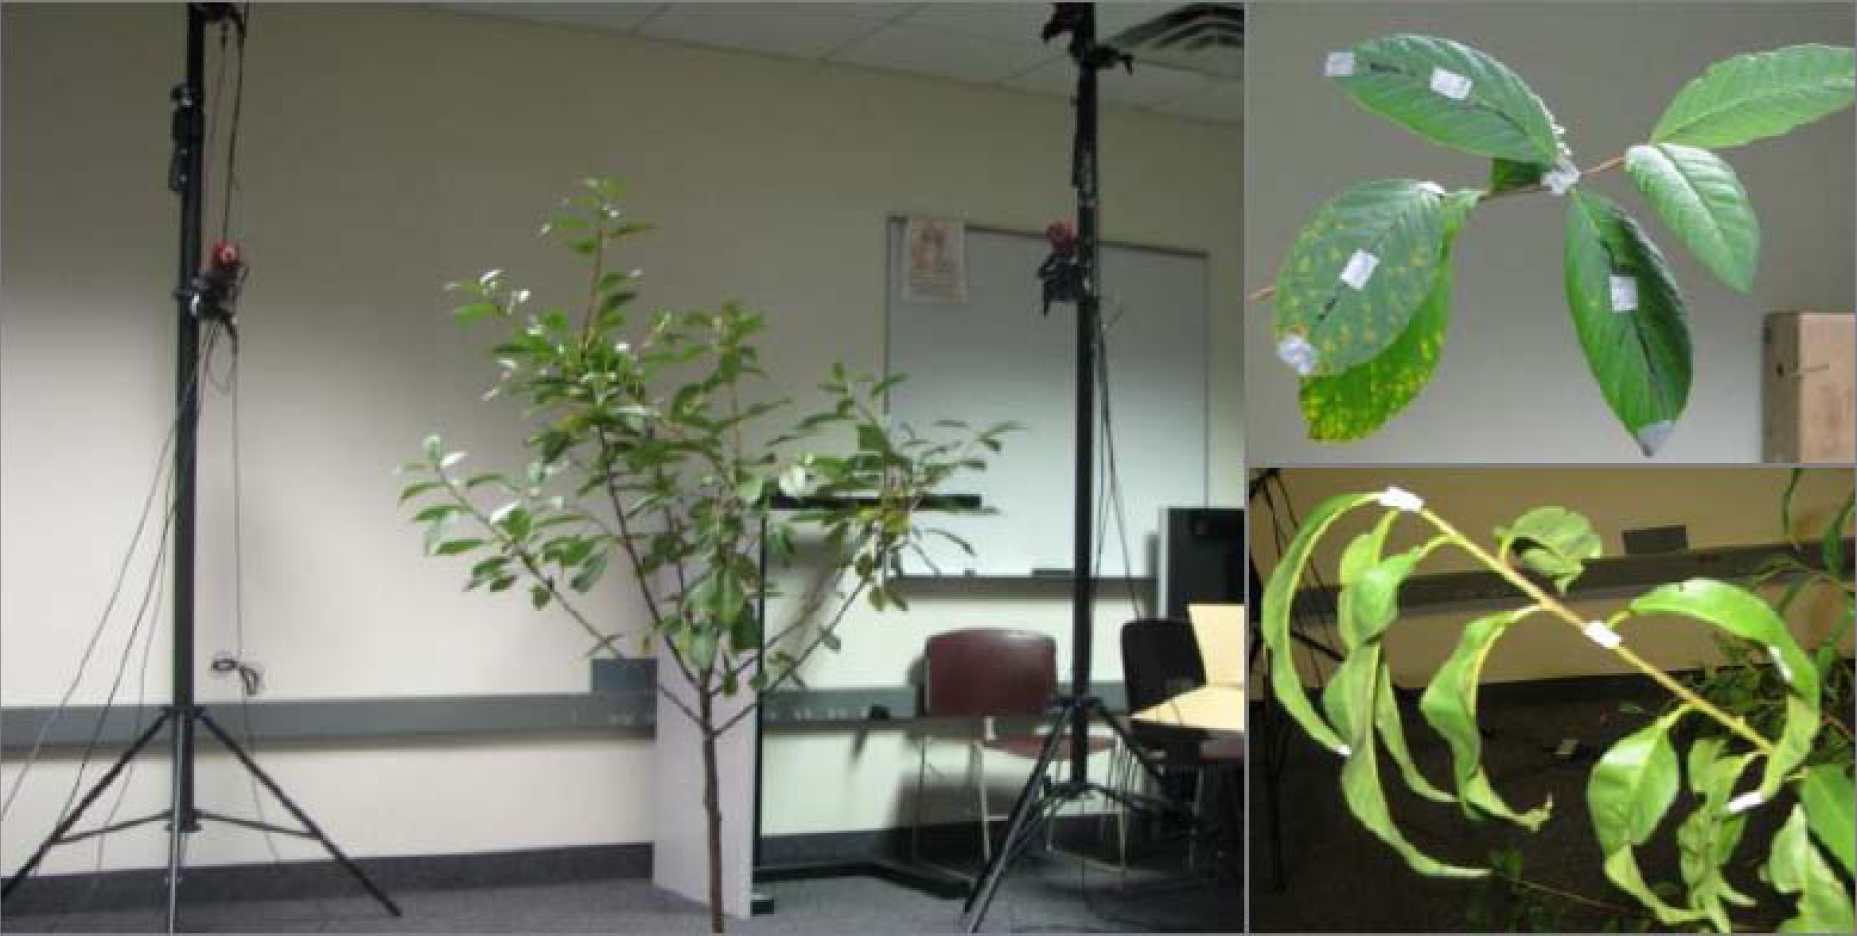
\includegraphics[width=6.0in]{experiment.PNG}
\caption[Motion capture set up for a natural tree.]{Motion capture setup for a natural tree using an optical motion capture system. }
\label{fig:Setup} 
\end{figure}

\section{Build Static Tree Geometries} 

One significant problem with motion capture of trees, compared to human performance capture, is that the branching structure, or topology, of a tree is less predictable and more complex than that of a human.  A minimal spanning tree algorithm is used with a cost function derived from motion data to create a plausible branching structure.  The branching structure is plausible when animating it with the captured motion looks plausible. The cost function is one of the contributions of this paper.  

\subsection{Skeleton and Topology Estimation} 

\begin{figure}[tb]
\centering
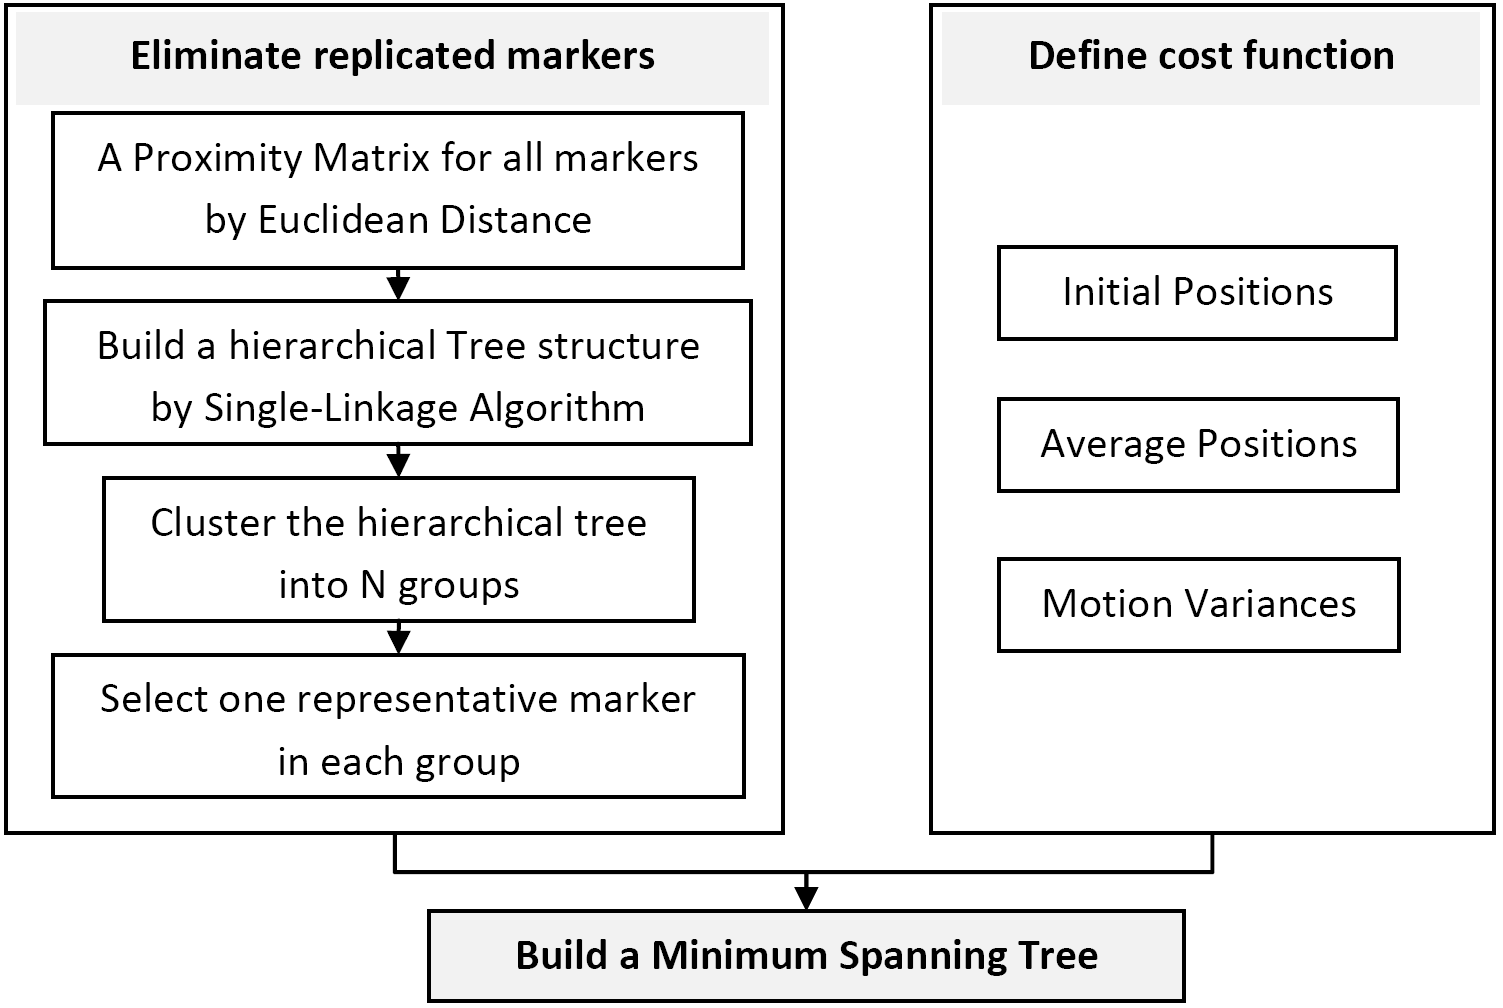
\includegraphics[width=5.0in]{skeleton.PNG}
\caption{Steps in building a tree skeleton.}
\label{fig:Skeleton} 
\end{figure}

Figure~\ref{fig:Skeleton} summarizes the process of estimating the skeleton and topology. This process has three steps. First, hierarchical clustering eliminates replicated recorded markers in each frame. Next, we use position and motion data for each marker to define a cost function.  The cost function is used to estimate the plausibility of merging two different markers. A minimum spanning tree algorithm uses a different cost function to connect the markers into a tree-like skeleton that will have plausible motion when animated using the captured motion data.

The first step, shown on the left side of Figure~\ref{fig:Skeleton}, is to eliminate duplicate, yet slightly different, recorded positions of a single marker.  We use Euclidian distance as the clustering metric. The single linkage algorithm groups markers into a hierarchy of $n$ clusters, where $n$ is the number of markers originally placed on the tree.  Within each frame, a cluster is reduced to a single representative marker.  When all frames have the correct number of markers, we further refine the representative position of each marker, either by choosing its position in the tree's rest pose or by averaging its position over time. The tree skeleton is built from the $n$ representative marker positions.  This skeleton is used for the entire capture sequence.

The second step, shown on the right side of Figure~\ref{fig:Skeleton}, computes costs for creating connections in the control skeleton between different pairs of markers based on the recorded position and motion data. Connection costs are computed for pairs of representative markers with one marker from each cluster. The cost function consists of three elements: initial position, average position over time, and variance of position over time. We assume that the branch motion is periodic. The  average position is similar to the position while the variance reflects the amplitude of the movement. The initial positions are recorded when there is no wind and the tree is stationary. The average positions are calculated as shown in the next equation in which $m$ is the number of recorded frames and $p_i$ is the 3D position for a marker at the $ith$ frame: 
\[
	   \bar{d} = \frac{1}{m}\Sigma_{i=1}^m p_i.
\]
The variance in position is similarly defined as 
\[
      \sigma^2 = \frac{1}{m}\Sigma_{i=1}^m (p_i-\bar{d})^2.
\] 

Let $\alpha$, $\beta$, and $\gamma$ be constant weighting parameters; then the cost to connect markers $M_a$ and $M_b$ is given by
\[
      \omega = \alpha||p_{M_a} - p_{M_b}|| + \beta||\bar{d}_{M_a} - \bar{d}_{M_b}|| + \gamma||\sigma_{M_a} - \sigma_{M_b}||. 
\]

The cost to connect markers $M_a$ and $M_b$ is low when $M_a$ and $M_b$ are close in both position and movement.

In the third step, we use Prim's MST algorithm with the node at the bottom of the trunk as a starting point to build the tree skeleton. Pairs of markers with similar position information and movements have low connection cost and are connected in the skeleton. This skeleton is directly taken as the input tree structure for rendering in the next step.    

Figure~\ref{fig:costResults} shows the importance of each part of the cost function. The right side of Figure~\ref{fig:costResults} shows a tree created using just the change in variance as the cost function. This cost function results in branch tips connected to branch tips because variance increases as one moves along a tree from trunk to branch tips. The middle tree was created using only positional information.  While the structure is accurate for much of the tree, several points are connected incorrectly across the middle of the tree. This will result in implausible motion when animated using the motion capture data. Using both metrics, along with average position, results in a more accurate model shown on the right.  

By combining these parameters, we connect markers with similar position and movement. For a tree with 98 clusters of markers, 66.26\% of the resulting connections are correct when compared with the actual tree. Most errors are from connecting markers in the correct branch segments but at the wrong junction points within the branch segment.   This cost function occasionally connects markers from different branches but which share close positions and movements.  In these cases, the motion of physically adjacent branch tips is similar and the resulting animation is still plausible.  

\begin{figure*}[tb]
\centering
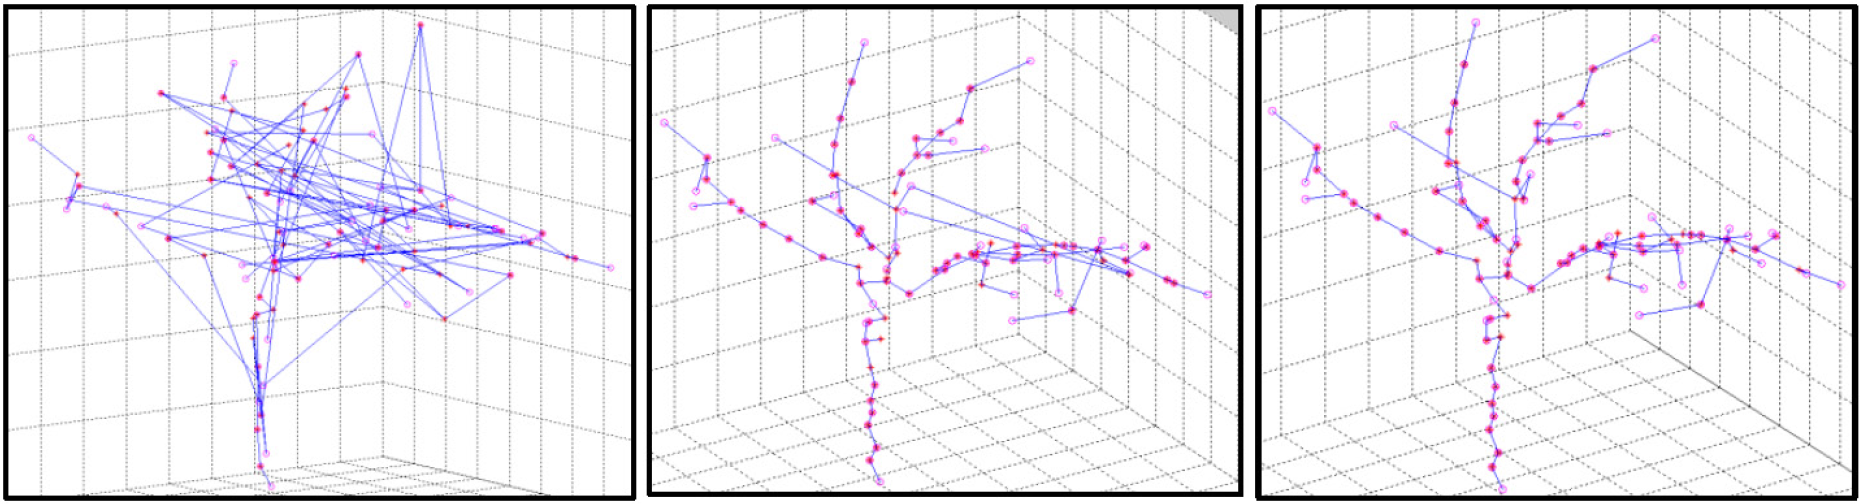
\includegraphics[width=6.0in]{cost.PNG}
\caption[Reconstructed tree topologies.]{Reconstructed tree topologies using variance, initial position, and a combination of variance, initial position, and average position.}
\label{fig:costResults} 
\end{figure*}

\subsection{Geometry of Branches and Leaves}

After the tree skeleton is created, the next step is to generate the geometric mesh. The marker points in a single branch are used as control points to create a curve. A second curve is placed at the first marker point in the branch and oriented to the first two points in the branch.  A closed circular shape is swept along the profile curve to create a NURBS surface. The profile and shape curves are discarded, leaving just the branch geometry.

Then we bind the mesh to the skeleton.  This step is separated from the previous steps so that the artist has more flexibility to modify the automatic mesh before it is bound to the skeleton. After any needed updates, the mesh is bound to the geometry. Once the geometry is bound, the artist again has the flexibility to manually tweak the binding.

Finally, a 3D point cloud inferred from photographs guides the manual placement of leaves. The leaves are placed to fill the volume occupied by the original tree. The tree volume is created using inverse volumetric rendering \cite{RecheMartinez2004} applied to 37 photographs taken from a known camera position. The resulting 3D point cloud is exported to a 3D modeling package and, after manually matching the tree skeleton with this point cloud, we manually place leaves on branches while remaining in the recorded crown volume.

\section{Build Tree Motion} 

In this section, we describe branch motion repair and leaf motion synthesis. Branch motion repair is the process of identifying and eliminating errors, gaps, and noise from the motion capture data. The resulting motion is used to animate the 3D tree model created in the prior section. 

We used the rigid body algorithm that was shipped as part of the NaturalPoint Arena software to convert unindexed point clouds into an animated skeleton. Because tree branches are non-rigid at large deflections, the resulting motion contains more gaps and errors than one might expect to find for rigid body motion capture. We use linear interpolation, a filter, and a machine learning algorithm to repair the resulting motion. The NaturalPoint Arena software provides some interpolation processes to fix motion gaps, but requires the user to manually identify gap regions and select a correction method. We automate gap detection and correction with different methods, depending on the gap size.  A machine learning based method for addressing large gaps is one of the contributions of this paper.  We use a standard curve fitting technique for small gaps. 

\subsection{Filter-based Noise Detection and Removal}

For some non-rigid motion, the rigid body motion capture system introduces anomalous artifacts to the motion signal, resulting in sporadic popping motions of certain leaves and twigs. These artifacts are detected using convolution-based filtering techniques and are replaced by fitting Bezier curves over the corresponding sections of the motion signal.  

\subsection{Small Gaps in Data}

Small gaps in data are short sequences of 100 frames or less in which no position data is recorded for a marker.  Small gaps occur when a marker becomes occluded or is otherwise lost.  Linear interpolation is used to repair small gaps because linear interpolation can be done quickly and is good enough for these gaps. 

Linear interpolation predicts missing marker positions based on the positions of neighbors. For a marker with missing position data, we find the two nearest neighbors with available position data. Then we compute Euclidean distances among the positions of these three markers and a velocity for each marker. Different distance metrics can be used. By doing linear interpolation according to the positions and velocities, we estimate the position for the missing marker. 

Linear interpolation works well if all three markers have similar movement. However, if the motions of two different, but adjacent, missing markers have their positions interpolated from the same set of nearby neighbors, the resulting interpolated motion may not preserve each marker's unique periodic motion. This may happen even though we aim to make the interpolated motion fit smoothly with the existing motion for each marker. However, losing periodic movements for a short period of time when repairing a small gap still results in visually plausible motion. 

\subsection{Large Gaps in Data}

Repairing large gaps in data is done using a more sophisticated interpolation scheme so that the synthesized motion has good periodic properties.  Large gaps in data refer to gaps which comprise more than 40\% of the entire motion trace collected for a single marker. A machine learning algorithm builds a function that is used to infer motion that is used to fill large gaps.  

Given the connection between two adjacent markers, motion data for both markers at low wind speed, and motion data for one marker at high speed, the machine learning algorithm trains a support vector machine (SVM) and defines a correlation function. This approach is based on the observation that good data is captured for all markers at low wind speed, but large gaps appear in the data for some markers at high wind speed.  The SVM learns a correlation between data from two markers collected at low wind speeds.  This relationship is used to estimate missing motion at high wind speeds under the assumption that the relationship is not sensitive to wind velocity.

The tree skeleton structure is used to find the nearest topological neighbor with motion data for both high and low speeds. In most cases, markers at branch tips have missing data while markers at the branch base have the required data. This is because markers at the branch base move more rigidly than markers on tips. In these cases, the marker at a tip has large gaps in motion data and its nearest neighbor in the direction of the branch base often lies on the same branch.

Sequential minimal optimization (SMO) \cite{keerthi:nc01,platt:mit99} trains an SVM, which defines the correlation function between the two markers' positions at low speed. In order to improve the precision of the correlation function and to avoid phase differences, the motion data from each series is sorted in ascending order of displacement. Let $M_a$ be the nearest neighbor to $M_b$, which is a marker with missing motion at high speed. $M_a$ and $M_b$ both have motion data at low speed.  A learned function $F$ estimates the position of $M_b$ given $M_a$. Position data from $M_a$ recorded at high wind speeds is given to $F$, which then estimates $M_b$'s position at high wind speeds.  

Figure~\ref{fig:result_curve} shows the estimated and actual position for one marker at low and high wind speeds. The vertical axis is the displacement and the horizontal axis is the frame number. In this figure, the motion of marker $M_a$ at low wind speed, which is the topmost trace on the left, is used with the recorded motion of marker $M_b$, which is the lower trace on the left, to learn a function that predicts the position of $M_b$ given the position of $M_a$.  For comparison, we placed the predicted position of $M_b$ on the graph as well.  The predicted position of $M_b$ closely matches the actual position at low wind speeds.  At high wind speeds, shown on the right, we held back the recorded position of $M_b$ and predicted the position of $M_b$ in each frame given only the position of $M_a$.  The predicted position of $M_b$ at high speeds closely matches the actual position of $M_b$ but tends to overestimate the amount of displacement in $M_b$. 

\begin{figure}[ht]
\centering
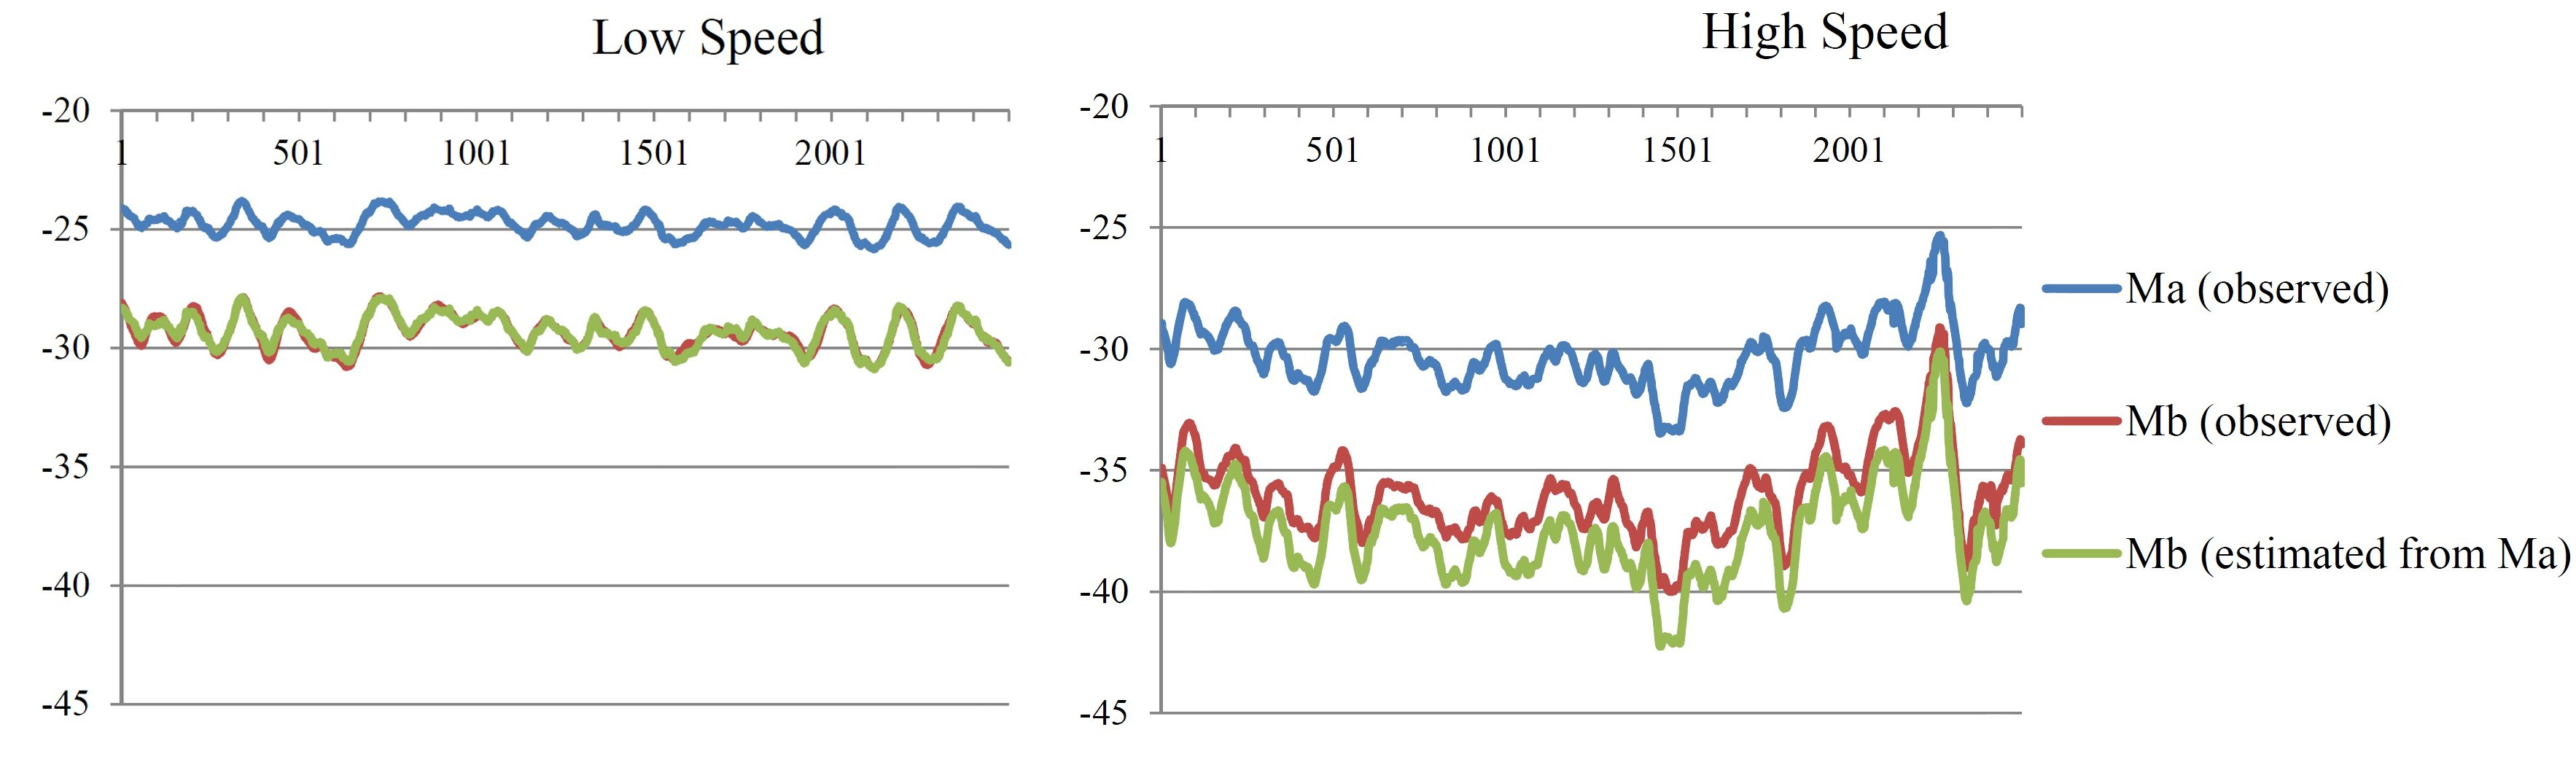
\includegraphics[width=6.0in]{low-speed-high-speed.jpg}
\caption[Predicted versus actual displacement.]{Predicted versus actual displacement for a marker at low and high wind speeds.}
\label{fig:result_curve} 
\end{figure}

\subsection{ Leaf Motions}

Motion data applied to leaves is based on motion captured from only a few leaves. This motion is scaled and offset to simulate a greater variety and randomness of leaf motion. The leaf geometry deforms along motion curves applied at the end, at the middle, and near the stem.

The complexity of leaves moving in the wind precludes any attempt to correlate leaf movement with the movement of the branch it is on. Leaves can be quite turbulent or almost still on a branch that is either very still or sweeping any position through its arcs of movement. However, motion of the leaves is scaled with the branch motion to suggest that they are driven by the same wind. These two motion sets can also be decoupled for an artist to achieve a particular effect. 

%\input{conclusion.tex} 
\section{Results} 

The final animation is shown in the video that accompanies this paper. In that video, most motion capture artifacts have been removed and the motion looks reasonable.  Results in skeleton estimation and motion repair, which are the main contributions of this paper, were given in the preceding sections.

%\input{futurework.tex} 
\section{Conclusion and Future Work} 

A plausible tree skeleton can be reconstructed using a minimal spanning tree algorithm over a cost function defined using position and motion data.  The skeleton is plausible in the sense that replaying the capture motion on the skeleton looks realistic.  Gaps and errors in motion capture data for trees can be replaced with data interpolated from neighboring branch motion.  These are important steps toward realizing motion capture of trees for tree animation in games.  Motion capture of tree motion is a good match for motion in games because the resulting motion is realistic but requires only replaying, rather than simulating, actual motion.  

We had hoped to get better results with the repaired data and the rigid body algorithm we used. Based on these results, we believe that investigating other approaches to processing the point cloud are more promising than repairing the errors caused by using the rigid body algorithm we used.  

Future work could take several interesting directions. One of these is to avoid defining rigid bodies for each branch while capturing motion by defining the tree as a non-rigid body, which is a truer representation of its natural form. More work needs to be done to be sure the algorithm scales well for capturing the motion of other tree subjects as well as for transferring captured motion from one tree to another. By capturing data from multiple trees at once, the interactions among them could be studied and applied to simulate groups of trees or even forests.
\chapter{Motion Capture of Rope}
\label{chap:rope}

\noindent
Jie Long, Bryce Porter, Michael Jones. Motion Capture of Rope.

\begin{abstract}
We reconstruct rope motion from passive optical motion capture data using a statistical model without a dynamic model of rope behavior.  Progress in motion capture for faces and cloth has limited applicability to the motion capture of rope because rope is a curved spline rather than a curved surface.  We present clustering, gap repair, and marker swap detection algorithms based on linear interpolation and forward differencing under the assumption that the rope does not stretch.  Indexed marker positions are connected with a spline in each frame to approximate the original rope.  The model produces visually plausible animations of rope motion from data collected for a person interacting with rope.  The method fails when the rope experiences large accelerations that result in motion that is not modeled by forward differencing. 
\end{abstract}

\section{Introduction} 

Motion capture for rope is a challenging problem because rope is a non-rigid body.  The problem is more difficult when the motion of a human character interacting with the rope is also captured in the same scene because, before markers are indexed from frame to frame, it is difficult to separate markers on the actor from markers on the rope.  We present a statistical motion estimation scheme with a clustering model to achieve motion capture of rope from passive optical motion capture data. Our solution consists of novel approaches to clustering and the repair of gaps and swaps, as well as segmenting rope motion from human character motion.

Motion capture of human characters interacting with rope may have applications in the production of computer-generated movies and video games.  Using motion capture data simplifies recording the interaction between characters and ropes while preserving the subtleties of that interaction.  Capturing interactions between rope and characters may be particularly compelling when motion capture is already being used to record character motion.  In this paper, we focus on separating rope motion from actor motion and then reconstructing the motion of the rope.  A variety of existing methods can be used to reconstruct actor motion from motion capture data.  The approach allows reconstructing the interactions between characters and thin, non-rigid bodies.

Prior work on non-rigid motion capture is mainly focused on facial motion (\cite{Lorenzo03,SifakisEftychios2005}) and cloth motion (\cite{MarcusVolker04clothmotion,whiteRyan2007siggraph,PritchardDavid2003,Bhat2003}). Both facial motion and cloth motion aim to build a mesh system for representing the motion of a surface. Motion capture of rope is a fundamentally different problem because rope is more naturally represented as a curved spline rather than as a curved plane (though a curved spline can be used to drive the motion of a plane). 

Human motion capture using a rigid body model (such as \cite{Lou:EHM2010,Wen:2006:MCD,Rajko:2007:RAK,ZordanVictorBrian2003}) is a well-studied area in motion capture but is less applicable to our research as removing the rigid body assumption changes the problem. Worring's \cite{WorringMarcel94measurementof} prior work in reconstruction of a line-shaped object in 3D from several computer images solves essentially the same problem but would require a foreground--background separation step and a sharp image of the rope in each frame.  
 
Our solution reconstructs free motion of rope and ribbon from recorded motion capture data. The captured data consists of an unindexed point cloud of purported marker positions. A marker segmentation algorithm is used to first separate the rope markers from the character so that the two motion streams can be reconstructed individually. A specialized clustering method processes the captured rope motion data and creates motion traces for markers in 3D space. Each cluster represents the motion from a single reflective marker. The clustering process also automatically detects and eliminates most noise. After creating these motion traces, marker swaps are detected and repaired by assuming that the rope does not stretch. Motion capture data marked as noise are revisited and used to fill gaps in marker traces if the data fits existing motion traces without extending the rope length. Small gaps are filled using linear interpolation and big gaps are filled using a structure-based midpoint displacement algorithm. Human character motion can be reconstructed using any of a variety of algorithms for reconstructing human motion from optical motion capture data.  The resulting motion streams containing rope and human motion, respectively, are recombined to recreate the original motion in 3D.

Our contributions are the following: \\
\indent (1) A marker segmentation algorithm that separates rope markers from the character markers.\\
\indent (2) A clustering algorithm to aggregate a point cloud into motion traces for non-rigid ropes and ribbons. \\
\indent (3) Forward differencing to estimate marker locations using previously labeled locations. \\
\indent	(4) A recursive midpoint displacement algorithm for fixing gaps.

These contributions allow us to recreate the interactions of a character with a rope or ribbon from passive optical motion capture data. Side-by-side playback of the resulting 3D motion and video of the original motion show that the captured motion closely matches the original motion.


\section{Related Work} 

The process of reconstructing motion from motion capture data includes data collection, data processing, and model mapping. Commercially available motion capture packages provide tools for creating the motion of a few objects, including human bodies and faces. Current research mainly aims to optimize the usage of collected motion data and to improve the quality of the resulting motion.  However, fundamental issues in the motion capture of non-rigid bodies require additional investigation.  

There are two common approaches to extracting human motion from motion capture data. One is to extract a skeleton model or kinematic model from motion data \cite{Lou:EHM2010,Rajko:2007:RAK}. The other is to predefine the skeleton and to apply motion capture data to animate the predefined skeleton \cite{Wen:2006:MCD,ZordanVictorBrian2003}. Wen \cite{Wen:2006:MCD} uses a least-square optimizing method to match motion capture data to a human skeleton. Zordan \cite{ZordanVictorBrian2003} maps motion capture data to a predefined skeleton using a force-based physical model. In our research, the structure of the rope model is a simple non-branching curve, so we predefine the rope shape and apply our algorithm to automatically map motion data onto the predefined structure.

Liu and colleagues \cite{Liu:tvcj06} take a data-driven approach to completing human motion from a limited set of markers.  A similar approach to rope motion reconstruction would require recording and analyzing many different rope motions, which could then be fit to partial data.  

Instead of a skeleton of rigid parts, non-rigid motion capture focuses on reconstructing a mesh that deforms to match a moving surface such as a face or cloth.  We also investigate non-rigid motion capture, but we focus on curved splines rather than curved surfaces.  

Motion capture for the human face is a well-studied problem.  Approaches that use 3D scans of face geometry \cite{bickel:siggraph07,park:tog06}, a model of the underlying tissue \cite{SifakisEftychios2005}, and displacement maps \cite{Ma:FPS2008,Lorenzo03} have been investigated.  These methods are not adequate for capture of rope motion because modeling deformed surface motion tracks a 2D surface rather than a 1D spline.  In practice a rope can undergo a wider range of motion, (such as coils, loops, and spins) than a face, but markers on rope are visible from all angles, unlike markers on faces, which are visible from only one side of the face.  

Motion capture for cloth is also a well-studied problem.  Prior work has been based on analysis of video of cloth motion, including customized texture patterns \cite{whiteRyan2007siggraph}, optical flow \cite{MarcusVolker04clothmotion}, a stereo pair of images \cite{PritchardDavid2003}, and finding simulation parameters based on video \cite{Bhat2003}.  As with motion capture of the human face, we have posed the motion capture problem for rope differently because rope has a different geometry and range of motions. 

A finite element model can simulate rope motion \cite{jiangWGIJMS1999}, including effects such as tension, shear, bending torsion, contact, and friction. Physical models for involve a parameter system to describe mechanics and structure and can be computationally intensive.

\section{Motion Capture Data} 

We use an optical motion capture system produced by NaturalPoint for recording data.\footnote{The system consists of 12 OptiTrack Flex:V100R2 camera mounted on light poles arranged in a circle with a radius of approximately 2.5 meters.} This section presents the notation used to describe motion capture data. 

\begin{figure*}[tb]
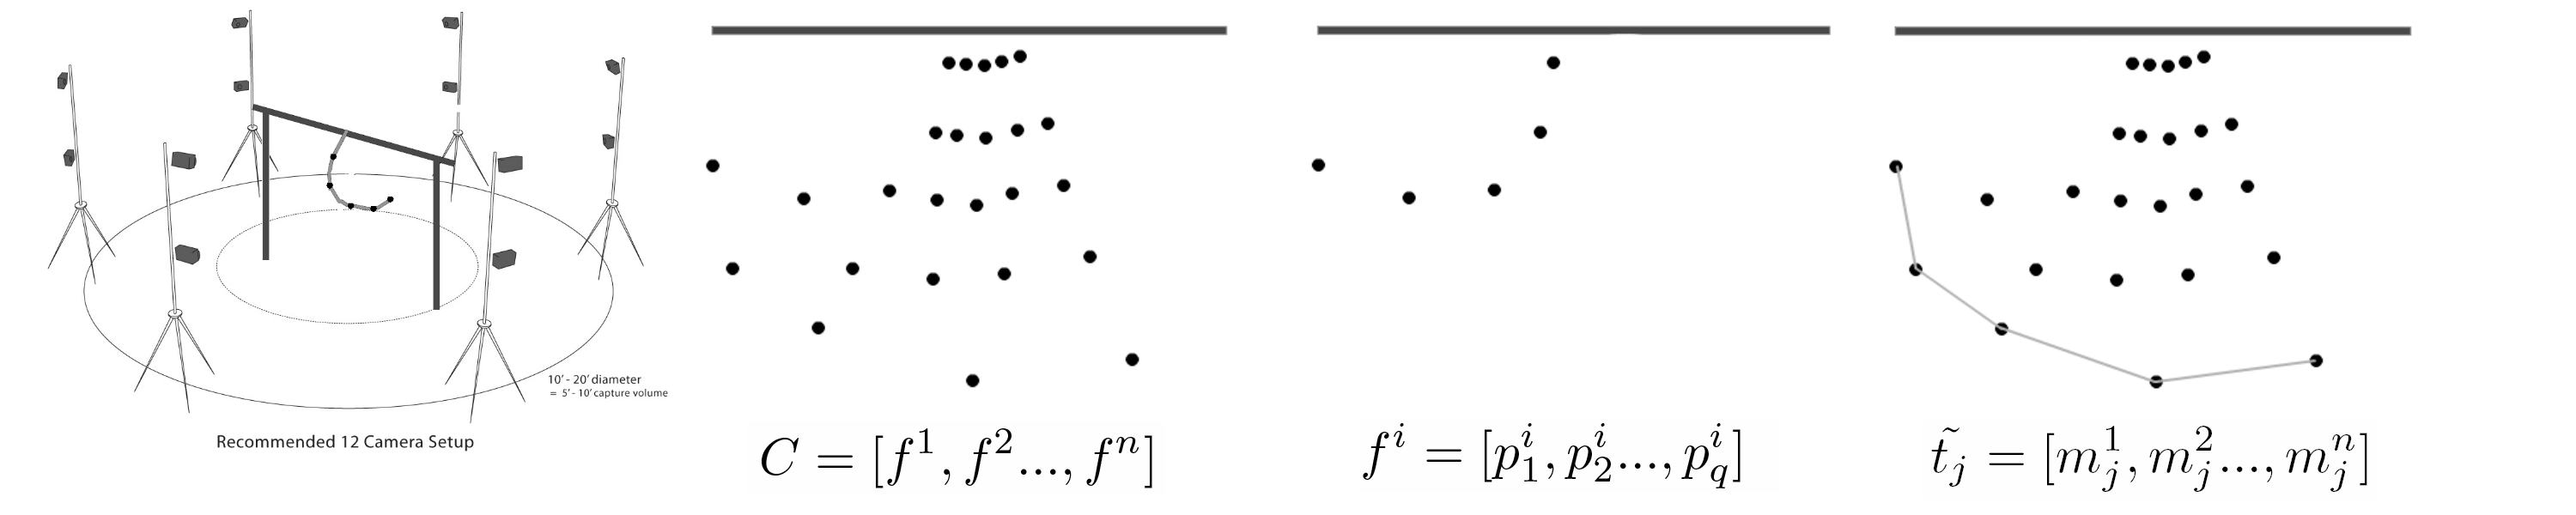
\includegraphics[width=\textwidth]{mocapData1}
\caption{Motion capture setup and notation for describing captured data.}
\label{fig:mocapData} 
\end{figure*}

After the motion capture arena is set up, an actor stands in the center of the arena. There must be enough space on all sides of the actor so that the rope can move freely and still be in the view of the surrounding cameras. Before recording the motion capture session, the actor assumes a T pose while the rope hangs vertically and separate from the actor.  This allows the marker segmentation and rope reconstruction algorithms to be initialized properly. After initialization, the actor can then interact with the rope. 

A motion capture session is $n$ frames of motion capture data:
\[
C=[f^1,f^2...,f^n],
\]
where each frame $f^i(1<i<n)$ consists of an unordered set of $q$ provisional marker locations:
\[
	   f^i=[p_1^i,p_2^i...,p_q^i].
\]
Each $p_j^i (1<j<q)$ denotes the $j$th marker position at frame $i$.  Figure~\ref{fig:mocapData} illustrates these concepts.  The left image shows a motion capture setup with a rope dangling from a pole in the center of an arena.  The next image shows a complete capture session, $C$, consisting of $n$ frames of data.  Next, the marker positions recorded for a single frame $f^i$ are shown.  Finally, the light gray line connects positions in a trace, $t_j$, of the position of a single marker across frames.  

In the following expressions, the superscript $i$ of $p_j^i$ always denotes the frame number. A provisional marker location $p_j^i$ is a triple denoting a 3D position in space. A marker location $m_j^i$ is the location of a specific marker with index $j$ in frame $i$. An initial trace, $\tilde{t_j}$ is an incomplete estimate of the position of a single marker over time and is a list of marker locations. 

\[
\tilde{t_j}=[m_j^1,m_j^2...,m_j^n]
\]

A final trace, $t_j$, is an initial trace after processing to repair gaps and undo marker swap.

In a single trace, a gap is a sequence of frames for which no provisional marker locations were assigned. Gaps are caused by either occluded markers or failure to assign a marker location to a trace.  The position of marker $j$ for which a position is not unknown in frame $p$ is denoted by $m_j^p=\bot$ as a gap. 

Noise occurs when marker locations are created based on transient reflections in the capture arena. Noise that creates motion outside our assumptions about rope motion is automatically detected and eliminated during data processing.

\section{Reconstructing Rope Motion} 

Rope motion can be reconstructed from unindexed marker positions using forward differencing and a novel midpoint displacement algorithm without a physical model assuming that the rope does not stretch. Our aim is to reconstruct rope motion from unindexed motion capture data in the presence of noise and a human actor. 

The main process is shown in Figure \ref{fig:mainProc}.  Markers on the rope are first separated from markers on the human actor so that markers tracking rigid bodies (such as the human actor's bones) can be processed separately from markers tracking non-rigid rope. The separation process is described in Section \ref{segmentation}; that section also shares ideas  from the reconstructing process. The unindexed points remaining after separating rope and actor motion are likely to represent markers attached to rope and are labeled into separate traces using a nearest-neighbor based clustering algorithm. All traces are assigned to a rope structure with a predefined length. Marker swap and gaps in motion traces are detected and repaired using statistical analysis along with the assumption that the rope does not stretch. Provisional marker locations not included in a trace in the first pass are classified as noise but may not be noise. After the first motion reconstruction pass, markers classified as noise are added to existing traces if they match the rope structure and motion. A post-processing step checks rope length and guides another round of processing if necessary. The process iterates until gaps, noise and rope stretching fall below acceptable standards or the algorithm fails to converge. In our research, some data, especially those with swaps and gaps, required two or three rounds of processing, but most of the collected motion capture data required only one round of processing and the algorithm did not converge for data with noise and many large accelerations of the rope.

After all motion capture data are matched into traces while noises and gaps are fixed, a Catmull-Rom spline connects all marker positions and creates a smooth curve among these positions on a rope.

\begin{figure*}[tb]
\begin{center}
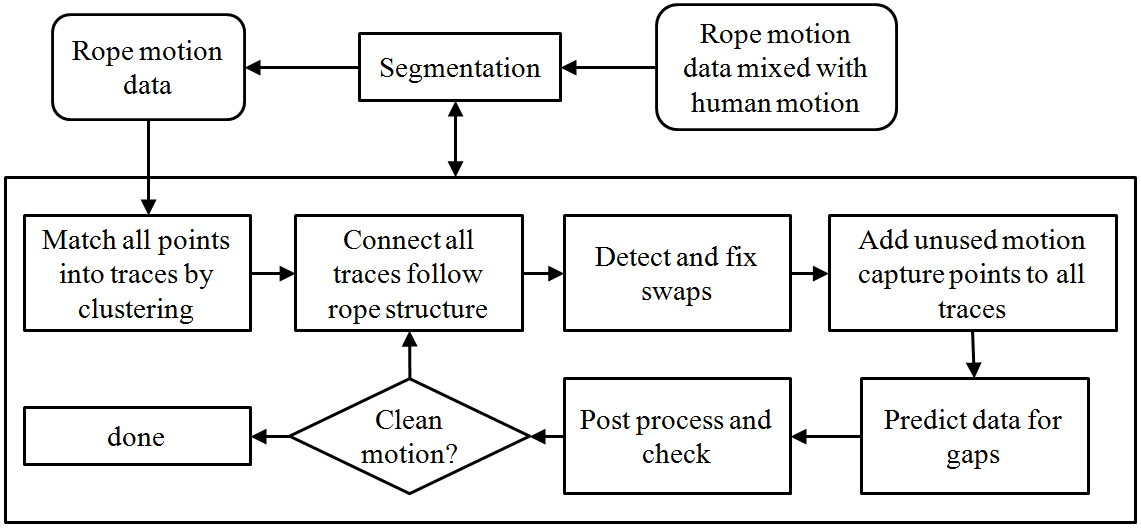
\includegraphics[width=5.5in]{mainProc.PNG}
\end{center}
\caption{Process for converting unindexed marker positions into motion paths.}
\label{fig:mainProc} 
\end{figure*}

\subsection{Clustering Positions into Traces}
\label{secClustering}

For frame $f^i$ and initial trace $\tilde{t_j}$ we attempt to find a provisional position $p_x^i$ that is a good match for $\tilde{t_j}$ in that frame.  If no match is found, we set $m_j^i=\bot$.
\[
m_j^i=\left\{\begin{array}{ll}p_x^i & \ \ \ \ \ \mbox{if $p_x^i$ is a good match for trace $\tilde{t_j}$ in frame $f^i$}\\
\bot & \ \ \ \ \ \mbox{otherwise}\end{array}\right.
\]

First, a small portion of the capture session with little or no movement is processed in order to find the number and locations of markers. Next, a second round of clustering assigns provisional marker positions across all frames to zero or one of the identified traces.  Positions not assigned to a trace are marked as noise and may be added to a trace later.  Each round of clustering is discussed in detail below.  

\subsubsection{First Round of Clustering}
The first round of clustering is performed on a stationary prefix session in which the markers remain stationary for approximately one second. This is similar to capturing a T pose during a motion capture session with a human actor.  

Two parameters, $\gamma$ and minPoints, are predefined. Parameter $\gamma$ is a 3D vector of the maximum allowable movement range for a marker during the stationary prefix.   Parameter minPoints is a threshold for the minimum number of provisional marker locations that must be assigned to a trace for that trace to be retained in the next round. A trace set $T$ is initialized by separate initial traces $\tilde{t_j}$ as 
\[
T={\tilde{t_1},\tilde{t_2},\tilde{t_3}...}. 
\]

In frame $i$, a position $p_x^i$ is appended as a marker location to trace $\tilde{t_j^i}$ when it is the closest provisional marker location to the average position of all the previous marker locations in a trace and it is within the threshold $\gamma$. If no such provisional location exists for a trace $\tilde{t_j^i}$, a gap $\tilde{t_j^i}=\bot{}$ is marked for trace $j$ in frame $i$. When a provisional marker location $p_x^i$ is not appended to any trace, a new trace $\tilde{t_j^i}$ is initialized with $\tilde{t_j^i}=p_x^i$. After all provisional marker locations are processed, traces which have fewer recorded positions than the threshold minPoints are discarded and the positions are marked as unused data for future analyses. 

\subsubsection{Second Round of Clustering}

The second round of clustering matches markers to traces using forward differencing (FD) to predict future marker locations. FD with order $s$ predicts an expected position $D_j^i$ for trace $\tilde{t_j^i}$ in frame $i$. Differencing $\Delta_j^s$ is computed with order $s(s>0)$ for trace $\tilde{t_j^i}$ from the previous frames $(i-s)$ to $(i-1)$:

\begin{equation}\label{eq:1}
\Delta_j^s=\Delta^sm_j=\sum_{w=1}^s(-1)^s\left(\begin{array}{c}s\\w\end{array}\right)m_{j+s-w}.
\end{equation}

After getting the differencing values $\Delta_j^s$, the predicted new position $D_j^i$ for trace $j$ in frame $i$ is estimated as 
\begin{equation}\label{eq:2}
D_j^i=\sum_{w=0}^s\left(\begin{array}{c}s\\w\end{array}\right)\Delta_j^wm_{j}^{i-w}.
\end{equation}

The predicted position $D_j^i$ preserves motion continuity from the previous $s$ frames in trace $t_j$. Finding a new provisional marker position in the neighborhood of the predicted position $D_j^i$ is more precise than searching in the locus of the average position because the expected position varies with velocity and acceleration.  

However, large accelerations can result in a predicted marker position that is at a different location than the actual marker.  If the actual marker lies outside the neighborhood of the predicted position then the marker will be missed, a gap will be created in the trace, and the marker position will be marked as noise.  Later, after repairing gaps and swaps, it may be possible to insert the missing marker position into the trace.   

\begin{figure}[tb]
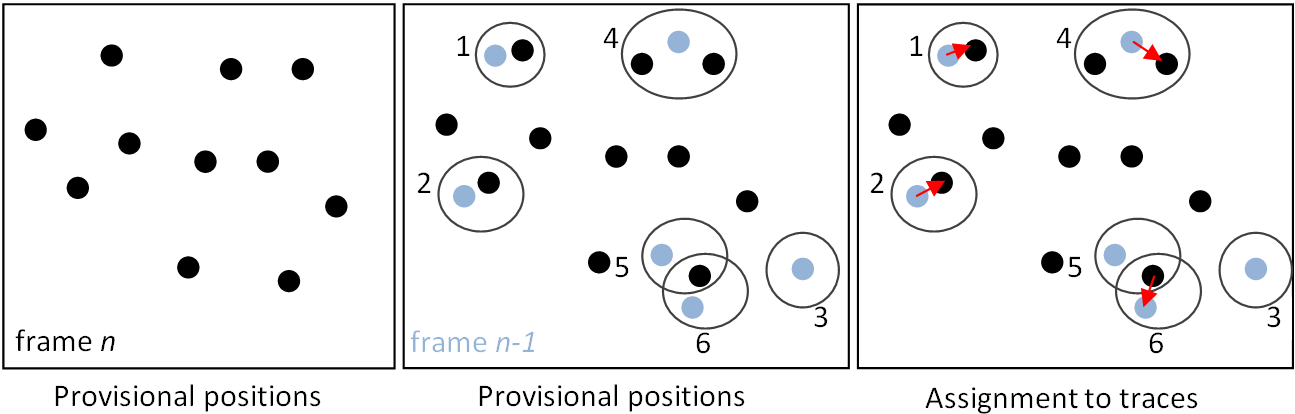
\includegraphics[width=\columnwidth]{ClusterProc.png}
\caption{Clustering process for the second round.}
\label{fig:ClusterProc} 
\end{figure}

Figure~\ref{fig:ClusterProc} illustrates the clustering process. The image on the left shows the provisional marker positions in $f^i$.  FD on markers 1 through 6 from $f^{i-s}$ to $f^{i-1}$, where positions of markers 1 through 6 from $f^{i-1}$ are shown in light gray, is used to identify likely positions of markers 1 through 6 in $f^i$.  These likely positions are called neighborhoods and are contained in the gray circles in the middle image. Next, for all marker positions $m_j^i$ in the neighborhood of $D_k^i$  compute:

\begin{equation}\label{eq:3}
\tilde{t_k^i}=m_j^i=min_{\forall{p_x^i}\forall{D_y^i}}\left\|p_x^i-D_y^i\right\|.
\end{equation}

A provisional marker location $p_x^i$ is appended to trace $\tilde{t_k^i }$ if $p_x^i$ is the nearest provisional marker location in the neighborhood $D_k^i$ predicted from trace $\tilde{t_k^i}$.  This is shown on the right side of Figure~\ref{fig:ClusterProc} as one of the provisional markers is assigned to traces 1, 2, and 4. In each case, the provisional marker location is assigned to a trace that has the nearest neighborhood $D_k^i$ to the location.  If no such $p_x^i$ lie within the forward differencing estimation then $\tilde{t_k^i}=\bot$. In Figure~\ref{fig:ClusterProc}, trace 3 is assigned to $\bot$ because no provisional locations lie close enough to the position of trace 3 from $f^i$.  A provisional marker location $p_x^i$ might be mapped to more than one trace---as is the case for traces 5 and 6 in the figure. In this case, the closest trace keeps the provisional marker location $p_x^i$ while the others are marked as having a gap. In this case, trace 6 is closer to the shared position and trace 5 is marked with a gap. If a provisional marker location $p_x^i$ is not clustered with any trace then that position is marked as unused data. The remaining black dots in the right side of Figure~\ref{fig:ClusterProc} are marked as unused data and may be assigned to traces later, which is discussed in Section ~\ref{sec:addUnusedSec}.  

Figure~\ref{fig:SecCluster} demonstrates a trace graph for 5 dangling ropes instrumented with 5 markers each. The left image is before clustering and the right is after. All traces are painted in different colors. Black circles indicate the stationary positions of each marker. Noise and unused data are detected but not shown in the image of the reconstructed traces on the right. 

\begin{figure}[tb]
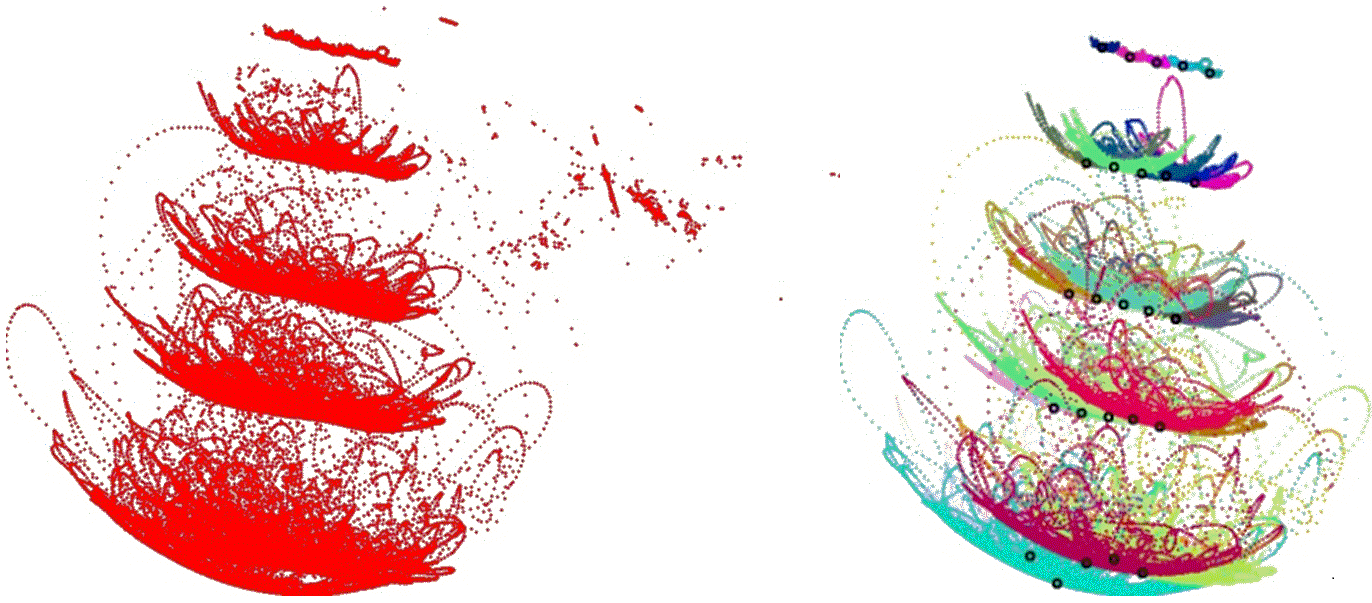
\includegraphics[width=\columnwidth]{SecCluster.png}
\caption{An input point cloud and clustering result.}
\label{fig:SecCluster} 
\end{figure}

\subsection{Swaps}

Marker swap occurs when marker positions are assigned to the wrong trace.  In our data, marker swaps occur at a rate of about one swap per thousand frames of data.  While swaps are uncommon, swaps lead to visually implausible animations, as the rope appears to twist and bend unnaturally.  In many cases, swaps lead to the appearance of the rope stretching. This is the key to detecting such swaps. A rope with length greater than the initial stationary length is called a stretched rope and likely indicates a marker swap.  

A segment is the span of rope between any two markers on a single rope. Stationary marker positions from the first round of clustering are denoted $\bar{m_x}$ and $\bar{m_y}$. With a distortion factor $\alpha$ for length error tolerance, a rope segment between markers $m_x$ and $m_y$ is considered stretched if
\begin{equation}
\left\|m_x^i-m_y^i \right\|>\alpha*\left\|\bar{m_x}-\bar{m_y}\right\|.
\label{eq:strech}
\end{equation}
The distortion factor $\alpha$ is small enough to detect swaps before they are visually significant. We set the value of $\alpha$ in [0.1,0.15]. 

We implemented two approaches for finding rope stretching: a case-based approach and brute force. The case-based method only checks rope length when there is a reasonable chance of swapping while the brute force approach checks rope length in every segment in every frame.
 
In the case-based approach, we collect candidate swapping points based on two assumptions: (1) when the distance between any two provisional marker locations is smaller than a threshold $minDist$ and (2) after a gap whose length is bigger than a threshold $maxGapLen$. After collecting all candidate swapping points, the segment length at a candidate swapping frame is checked using equation \ref{eq:strech}. After two markers approach in space, the following $N$ frames have higher probability of containing a swap because the clustering-based labeling process might swap positions.  Therefore, segment length is checked the $N$ frames after markers pass in close proximity.  A related segment is a rope segment that contains candidate swapping points.  A swap of two candidate points is detected and repaired if the potential swapping satisfies two requirements: (1) before the swap, both lengths of related rope segments are stretched, and (2) after the swap, at least one of these lengths is corrected.

In the brute force method, the rope length is checked in each frame using equation \ref{eq:strech} with a distortion factor $\alpha$.  When rope length is stretched in a frame, we try all permutations for all marker positions for all ropes in a scene.  Swap repair stops when all rope lengths are not stretched or when all permutations have been checked.  However, in the worst case, the number of permutations is in the order of $n!$, where $n$ is the number of marker locations. That makes this approach infeasible in most cases.

\subsection{Gaps}
\label{sec:Gaps}

Given a trace, a gap is a sequence of frames in which recorded marker positions were not assigned to that trace.  Gaps are repaired by filling gaps with estimated locations. A small gap has less than five continuous missing frames. Small gaps are fixed by linear interpolation. Fixing a large gap uses assumptions about rope shape, statistical characteristics of the marker and the movement of other markers on the same rope.  This section focuses on repairing large gaps.

A gap session is a span of time in which multiple traces have gaps. During a gap session, multiple traces might have gaps with different durations. Smaller gaps and gaps in traces with small ranges of motion (if any) are repaired first.

\begin{figure*}[tb]
\center
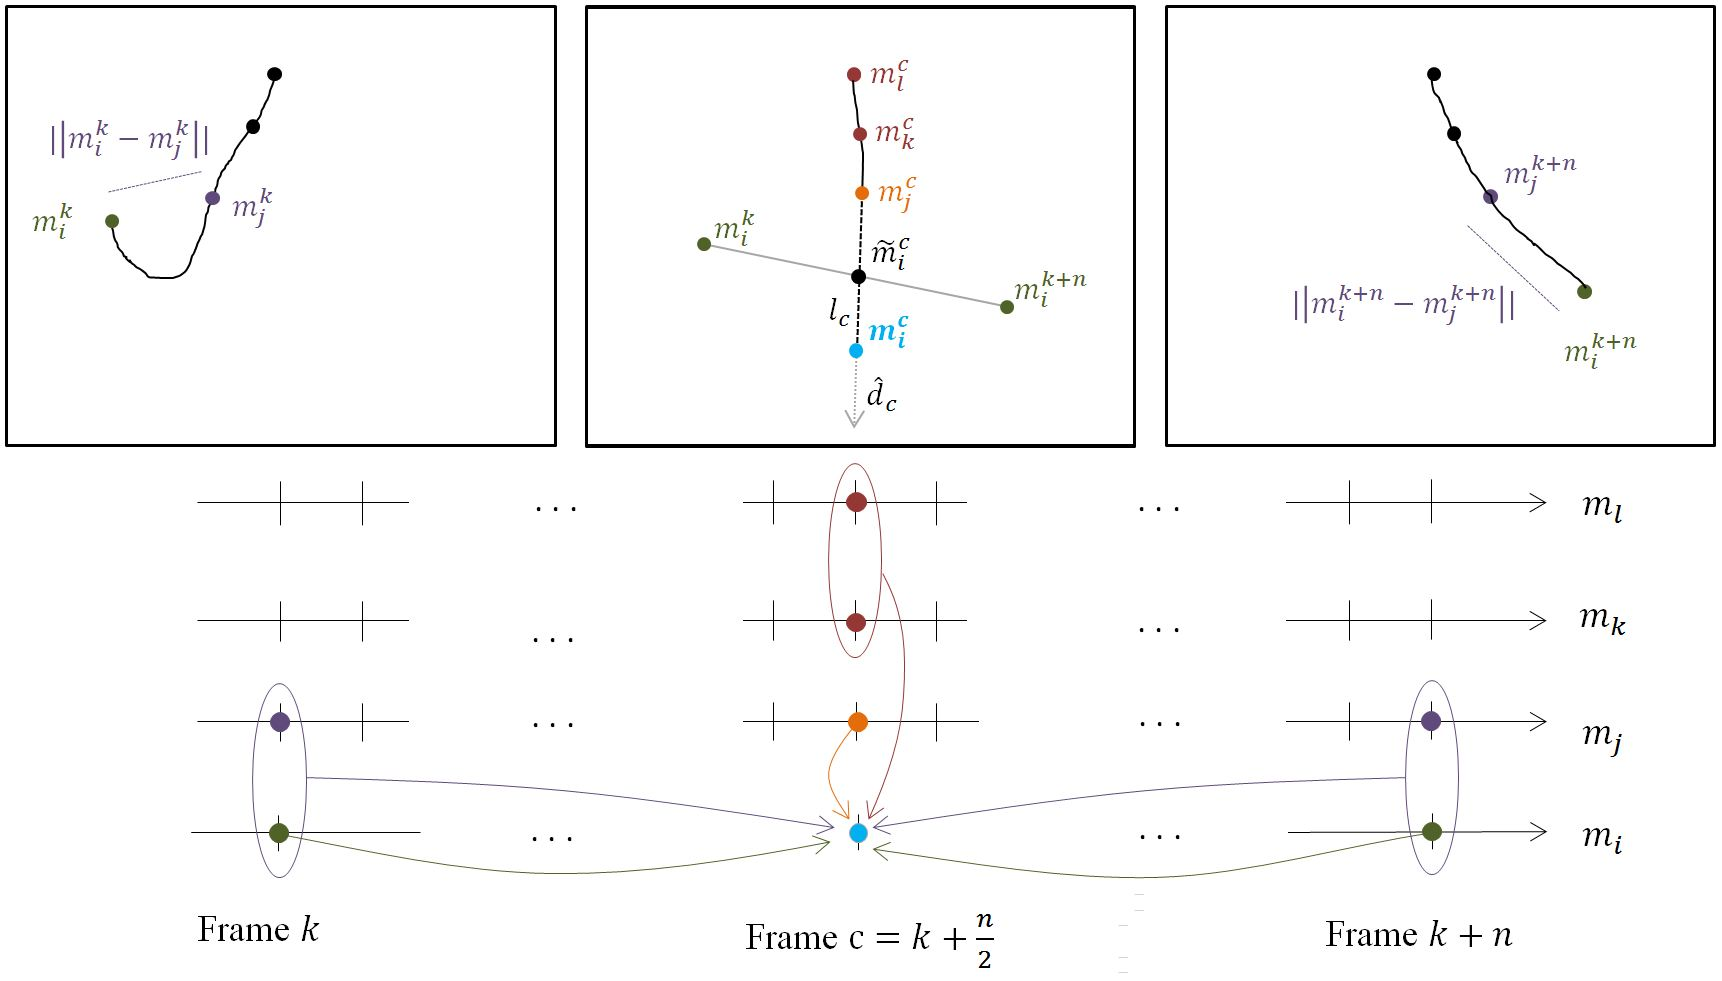
\includegraphics[width=1.0\textwidth]{filling-gaps-2.jpg}
\caption[Estimate the position of marker.]{Estimating the position of marker $m_i$ in the center frame of a long gap using the positions of markers $m_j$, $m_j1$, and $m_j2$.}
\label{fig:gapFix} 
\end{figure*}

A recursive midpoint displacement method estimates marker positions through large gaps. This process is shown in Figure~\ref{fig:gapFix}. Suppose the trace of marker $m_i$ includes a gap from frames $k$ to $k+n$ and that the trace of nearby marker $m_j$ is complete over the same span.  Marker $m_j$ is adjacent in the sense that it lies next to, or near, marker $m_i$ on the rope segment.  Figure~\ref{fig:gapFix} contains rope positions in the top series of frames, and timelines at the bottom of the figure show which marker positions in which frames are used to estimate the position of marker $m_i$ at the frame $k+n/2$ in the middle of the gap.  Marker locations in the top series of frames and the timelines are color-coded.  The process involves estimating the distance between $m_i$ and $m_j$, estimating the position of $m_i$, and then estimating direction from $m_j$ to $m_i$.  These estimates are generated from known marker positions in frames $k$, $k+2$ and the midpoint frame.  

The estimated distance between known markers for the segment at the middle frame, $l^c$ (where $c=k+n/2$), is computed by averaging the segment length between $m_j$ and $m_i$ (shown in purple in the figure) starting in frame $f_k$ and ending in frame $f_{k+n}$. 
\begin{equation}\label{eq:6}
l^c=\frac{\left(\left\|m_i^k-m_j^k\right\|+\left\|m_i^{k+n}-m_j^{k+n}\right\|\right)}{2}
\end{equation}   
The preliminary location of $m_i$ in frame $c$, which is denoted $\tilde{m_i^c}$, is the average of the locations of $m_i$ at the start and end frames. 
\begin{equation}\label{eq:7}
\tilde{m_i^c}=\frac{m_i^k-m_i^{k+n}}{2}
\end{equation}
The position of $m_i$ at the start and end frames is shown in green in Figure~\ref{fig:gapFix}. 

Next, the direction from $m_j^c$ to $m_i^c$ is estimated using the weighted sum of the direction from $m_j^c$ to $\tilde{m_i^c}$ and the direction between two other nearby markers $m_{j1}^c$ and $m_{j2}^c$ (shown in red in Figure~\ref{fig:gapFix}).   
The direction $\hat{d^c}$ is given by 
\begin{equation}\label{eq:8}
\hat{d^c}=Norm\left[\alpha*\left(m_j^c-\tilde{m_i^c}\right)+\beta*\left(m_{j1}^c-m_{j2}^c\right)\right],
\end{equation}
where $\alpha$ and $\beta$ are weighting parameters.   

Finally, the location of marker $m_i^c$ in frame $c$ is determined by moving a total of $l^c$ units along the normalized vector $\hat{d^c}$ starting at known marker location $m_j^c$:
\begin{equation}\label{eq:9}
m_i^c=m_j^c+l^c\hat{d^c}.
\end{equation}
The new position is shown in blue in Figure~\ref{fig:gapFix}. 

The midpoint displacement method proceeds recursively and fills data in all the gaps in the gap session. When length of a sub-session gap is fewer than 5 frames, it will be fixed using linear interpolation. 

\subsection{Add Unused Data}
\label{sec:addUnusedSec}

The unused data are revisited and added to existing traces if applicable. The nearest unused provisional location $p_y^{i}$ to a marker location $m_x^{i\pm1}$ in the neighboring previous or next frame fills a gap location $m_x^i = \bot$ if 
\begin{equation}
m_x^i=p_y^i=min_{\forall{m_x^i}\forall{p_y^i}}\left\|p_y^i-m_x^{i\pm1}\right\|,
\label{eq:addUnused}
\end{equation}
where $y\in{y_1,y_2,...y_z}$ and ranges over unused locations. 

The segment length resulting from using the closest provisional location $p_u^i$ is evaluated using equation~\ref{eq:strech}. If the segment is not stretched and equation \ref{eq:addUnused} is satisfied, the unused provisional location will be added in a trace to replace a gap $m_x^i$.

The process is repeated over the entire session. When there is a gap, the left and right ends of the gap are processed first because there are data available in the neighboring previous or next frames. This process is repeated for all gaps until no more unused data is added to a gap.

\subsection{Separate Rope Markers from Actor Markers}
\label{segmentation}

Rope motion captured with a human actor is separated from the actor's motion.  The segmentation is an important step in our method for recreating animation of an actor interacting with rope.  Rope markers are separated from markers on the actor after grouping markers into traces across frames.  The clustering method used to group markers is identical to the clustering method described above.   Alternatively, it may be possible and more desirable to separate rope and actor markers by tracking the actor skeleton as a collection of rigid bodies and classifying the remaining marker positions as rope markers.  

After the segmentation, rope motion is reconstructed from purported rope marker positions by repairing gaps and swaps and then adding unused markers as described previously.  To initialize rope marker locations, a user makes a simple selection of all and only the markers that belong to the rope, as shown in Figure~\ref{fig:SegInit}. 

\begin{figure}[tb]
\center
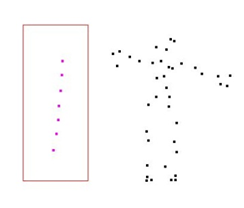
\includegraphics[width=3.6in]{segmentInitInverted.png}
\caption{Rope marker selection.}
\label{fig:SegInit} 
\end{figure}

As in Section \ref{secClustering}, at each frame we attempt to find a provisional marker location that is in close proximity to the next estimated position for a marker trace. When no provisional marker location can be found for a trace, instead of labeling a gap, we create a temporary marker for the marker trace. The temporary marker allows the algorithm to continue tracking a marker despite the presence of noise and gaps in the motion capture data.

In order to track a marker, we match provisional markers to traces using a linear combination of two predicted positions, $V_j^i$ and $N_j^i$. The first predicted position, $V_j^i$, is based on the last known velocity of the marker using equations (\ref{eq:1}), (\ref{eq:2}), and (\ref{eq:3}). The other position, $N_j^i$, is predicted using a midpoint displacement method, as described in Section \ref{sec:Gaps}, using equation (\ref{eq:6})--(\ref{eq:9}).

Then $V_j^i$ and $N_j^i$ are combined as follows:

\begin{equation}
F_j^i= \alpha V_j^i + (1 - \alpha) N_j^i,
\end{equation}

where $\alpha$ is one over the number of consecutive temporary markers. This means that the more consecutive temporary markers the trace has the less we rely on $V_j^i$, because it could have strayed too far from the actual rope markers. After fully segmenting the rope markers from the human markers it is possible to reconstruct the motion streams for each independently.

\section{Results} 

We present results that indicate that, under the assumption that the rope does not stretch, rope motion can be plausibly reconstructed from passive optical motion capture data without a physical model of rope dynamics.  This can be done in the presence of a human actor whose motion is tracked in the same capture session.  

Figure~\ref{fig:jumpRopeResult} shows the reconstruction of a motion capture session in which the character is jumping rope. Comparison with still frames taken during the capture session shows that both the marker segmentation and reconstruction algorithms accurately reproduce the original motion.

\begin{figure}[tb]
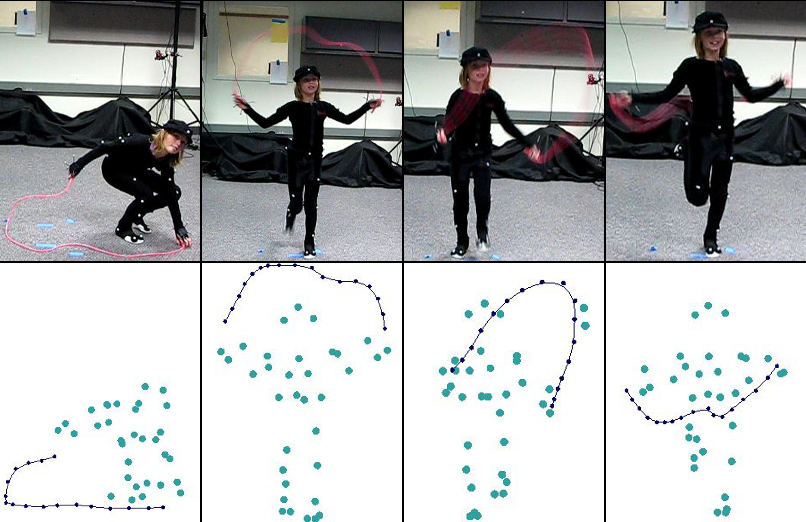
\includegraphics[width=\columnwidth]{jumpRopeFig.png}
\caption[Screenshots of original and reconstructed rope and human actor.]{Screenshots of the original motion, segmented rope and character markers, and the reconstructed rope with the human markers.}
\label{fig:jumpRopeResult} 
\end{figure}

Gap filling results in motion that is similar to missing motion in both magnitude and direction and has good continuity with surrounding motion.  Figure~\ref{fig:gapFillAnalysis} shows the average error for reconstructed marker positions for gaps created by holding back data from a motion capture session.  The horizontal axis shows the gap size in frames and the vertical axis shows the mean error for all frames in gaps of that size.  The data in Figure \ref{fig:gapFillAnalysis} were generated from 5,000 randomly generated gaps.  The curve is not smooth because of the random factors we included in the analysis. A gap created at different phases of a motion path might produce different values of error.

\begin{figure}[tb]
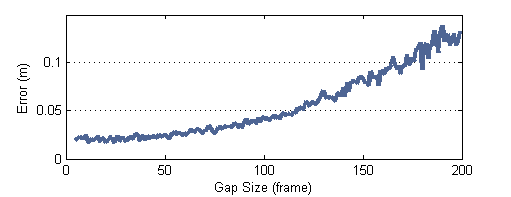
\includegraphics[width=\columnwidth]{gapAnalysisEasy50002.png}
\caption[Analysis of gap filling algorithm.]{Analysis of gap-filling algorithm. The horizontal axis is gap size and the vertical axis is error, which is the difference between the motion captured data after clustering and the data estimated by our method.}
\label{fig:gapFillAnalysis} 
\end{figure}

Figure~\ref{fig:Result} compares the original shape of the model with our results.  In the top row of Figure \ref{fig:Result}(a), we compare the ground truth motion data (left) with data generated by the gap-filling algorithm (right). The data shown in dash-dots on the left and right sides of each image is held back during gap filling. The synthesized motion, which is the bottom marker in solid lines on the right image of (a), preserves good continuity with existing motion and rope shape. Figure \ref{fig:Result}(b) shows traces (right) created from raw point cloud (left).

The process accurately extracts motion in a variety of settings.  Still images from both video taken during a capture session and reconstructed motion from that session are shown in Figure \ref{fig:Result}(c)--(f).  Each scenario is described subsequently, and complete video clips are included as reference material with this paper.

Five dangling ropes, as shown in Figure \ref{fig:Result}(c), have one end fixed to a horizontal support bar and rope motion is driven by hitting the ropes with a stick. This scenario is easy to process because one end of the rope is anchored to a fixed position in space and rope motions are relatively small. The resulting motion is smooth with few gaps and little noise.

We recorded a rope dropping from the horizontal support bar (shown in Figure \ref{fig:Result}(d)). The rope has one end fixed to the bar.  The rope is nudged over the edge of the bar using a stick.  This scenario is more complex than the five dangling ropes because the rope moves more quickly and with more bending.  We processed this data in inverse time order, so the structure of dangling rope is clearer at the end than at the beginning of the session . 

The motion of unanchored ribbons is more difficult to process because ribbons have less mass and are not anchored in this example.  Figure \ref{fig:Result}(e) and (f) show two frames from two sessions involving ribbons attached to a wand that is waved freely in the capture arena.  Ribbon is also more difficult because it is a lighter material that accelerates with less force than rope. By mapping different textures to the single ribbon motion, we create some interesting effects, such as animating lace cloth and a Japanese fish flag based on captured data.

\begin{figure}[tb]
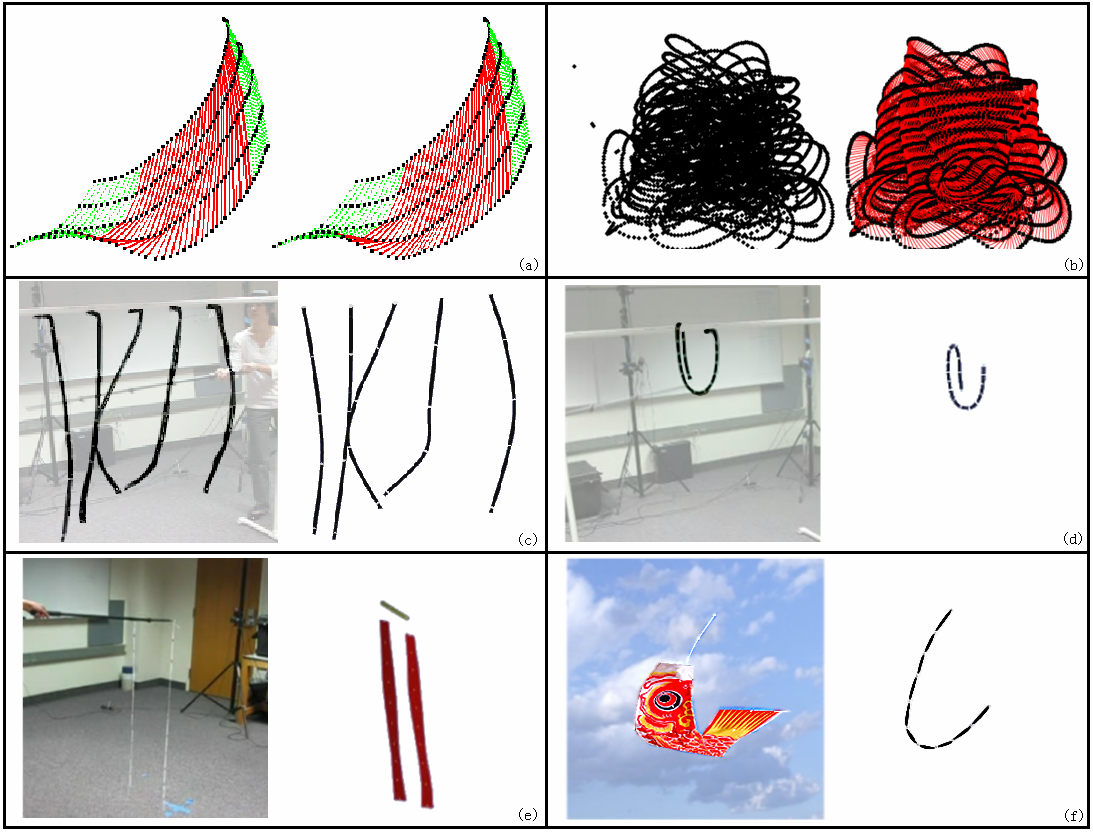
\includegraphics[width=\columnwidth]{result.png}
\caption{Screenshots of reconstructed motion of ropes and ribbon.}
\label{fig:Result} 
\end{figure}

\section{Conclusion and Discussion} 

Our work produces visually plausible rope motion from passive optical motion capture data using a statistical model under the assumption that the rope does not stretch.  The algorithm uses a novel clustering scheme, forward differencing, and a recursive midpoint scheme to automatically detect and remove most noise, gaps, and marker swaps.  The algorithm preserves continuity of motion in traces and fits the shape of rope.  This work lays a foundation for further investigation of motion capture for non-rigid bodies using statistical rather than physical models.  The approach to the problem may advance motion capture results for non-rigid bodies driven by complex or poorly understood physical systems.

Complicated motions (such as spirals, collisions, sudden changes in movement, or extremely fast movement) are not well handled in this model. Our assumptions for detecting swaps may be oversimplified relative to natural movement. Consideration of other factors, such as velocity or acceleration, might improve gap-filling results.  We have used a simple method for interpolating rope position between markers.  More complex methods may result in more plausible results particularly when the distance between markers on the rope is large.  

\chapter{3D Tree Modeling Using Motion Capture}
\label{chap:treeparticles}

\noindent
Jie Long and Michael Jones. 3D Tree Modeling using Motion Capture. \emph{IEEE The Fourth International Symposium on Plant Growth Modeling, Simulation, Visualization and Application (PMA '12)}, to appear.

\begin{abstract}
Recovering tree shape from motion capture data is a first step toward efficient and accurate animation of trees in wind using motion capture data. Existing algorithms for generating models of tree branching structures for image synthesis in computer graphics are not adapted to the unique data set provided by motion capture. We present a method for tree shape reconstruction using particle flow on input data obtained from a passive optical motion capture system. Initial branch tip positions are estimated from averaged and smoothed motion capture data. Branch tips, as particles, are also generated within bounding space defined by a stack of bounding boxes or a convex hull. The particle flow, starting at branch tips within the bounding volume under forces, creates tree branches. The resulting shapes are realistic and similar to the original tree crown shape. Several tunable parameters provide control over branch shape and arrangement.
\end{abstract}

\section{Introduction}

Reconstruction of tree shape from motion capture data is an important step in replaying motion capture of trees under external forces, such as natural wind. Motion capture provides a fast and easy way to collect the locations over time of retroreflective marker locations placed on an object. In this paper, we address the problem of creating 3D tree shape from motion capture data. We also discuss best practices for collecting motion data from a tree. This research focuses on reconstructing static 3D tree shape with branching skeletons from data collected by a motion capture system.

\begin{figure*}[!t]
\centering
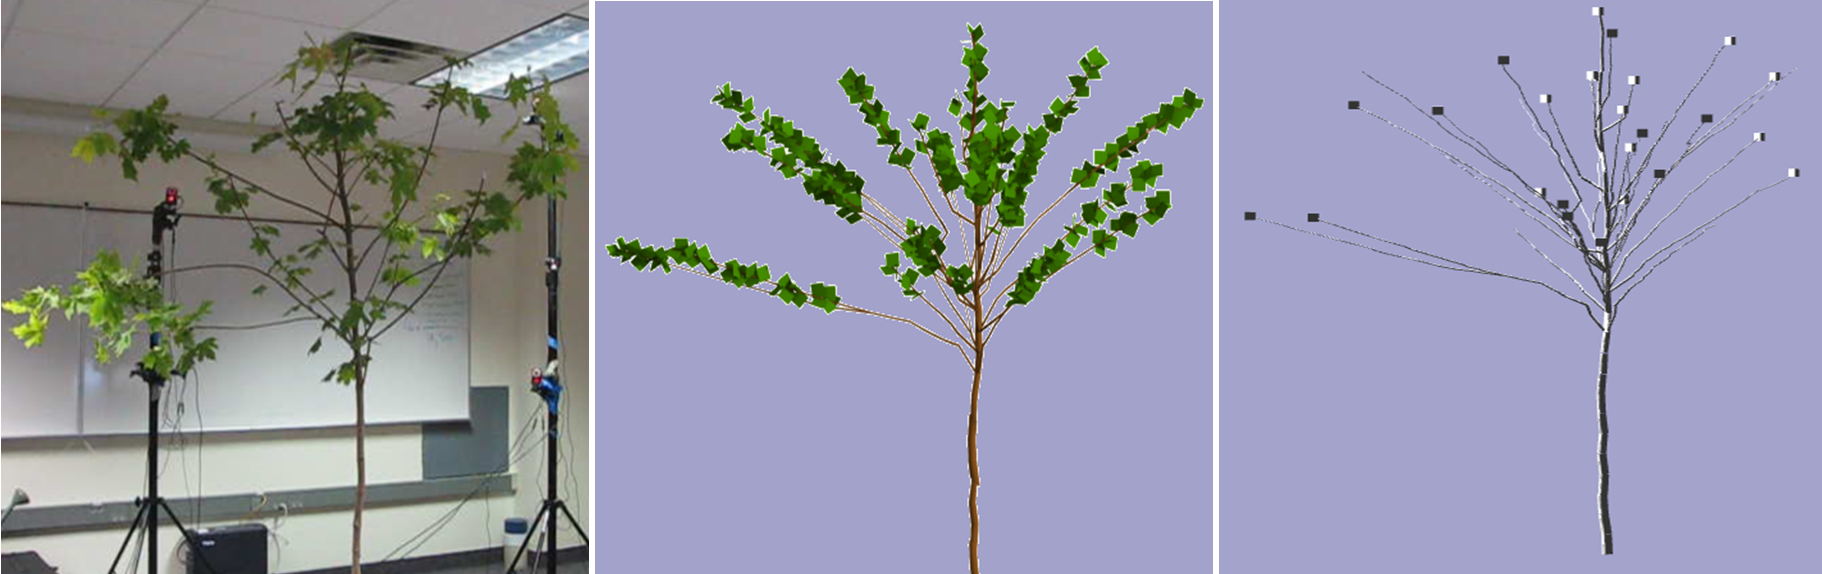
\includegraphics[scale=0.27]{Maple}
\caption{Maple model.}
\label{fig:treemodelssubfig2}
\end{figure*}

\begin{figure*}[!t]
\centering
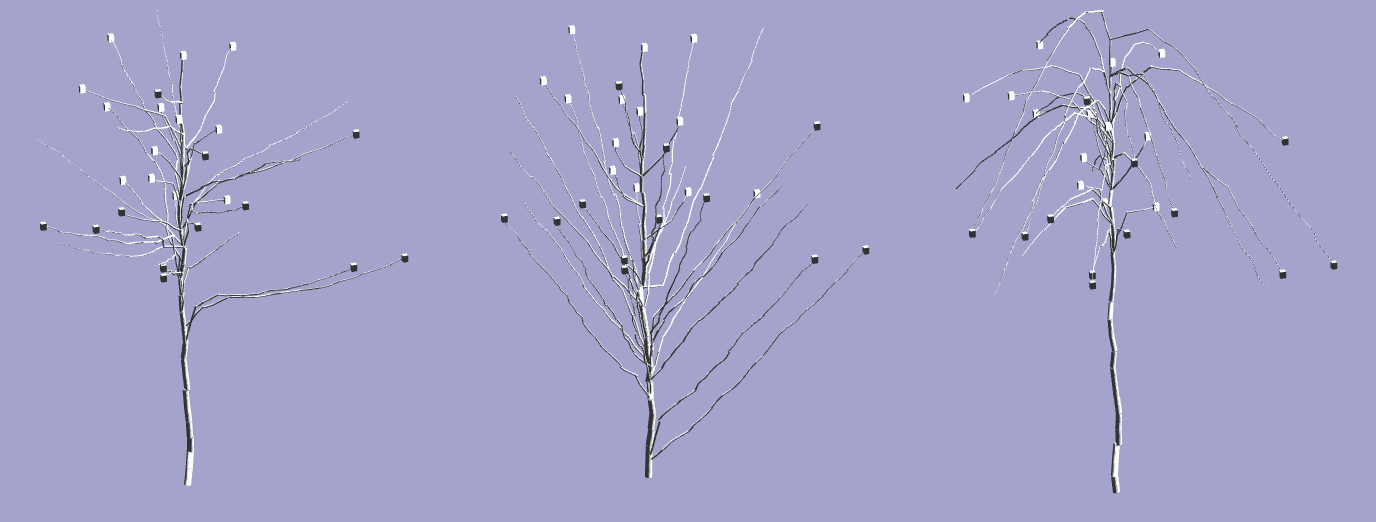
\includegraphics[scale=0.36]{varTree}
\caption{Various tree shapes generated from the same set of motion capture data. }
\label{fig:varTree}
\end{figure*}

Solutions to the motion capture problem for trees can be applied to problems in visual effects and the study of tree motion. Motion capture is a potential solution because motion capture data includes effects that are difficult to model in simulation, such as variable branch stiffness, non-uniform variation in size, and emergent effects due to leaf deformation.

Tree shape modeling has long been studied in computer graphics.  Past methods include particle systems \cite{Reeves83particlesystems,Runions07,palubicki:siggraph09,neubert:acmtg07}, L-systems \cite{lindenmayer68,Lintermann1999,Prusinkiewicz:2001}, parametric models \cite{Weber1995}, photographs \cite{RecheMartinez2004,neubert:acmtg07,Tan:2007:ITM}, and videos \cite{Li:2011:MGM,Diener:2006}. Most of these methods result in satisfying tree shapes but do not leverage the 3D positions of motion capture markers, which are recorded as part of a motion capture session but require a different set of inputs. Image- or video-based approaches convert a set of 2D input images into 3D tree models by filling in the missing dimension.  Motion capture systems can record tree shape in 3D with high precision (using similar techniques for converting a set of 2D images to a 3D model). Prior work in reconstructing tree shape from motion capture data using either exact measurements or markers placed within the crown does not scale and does not apply when leaves occlude the branching structure.

We reconstruct 3D tree shape using particle flow with motion capture data as input. Passive optical motion capture\footnote[1]{http://www.naturalpoint.com/optitrack/} records locations of reflective markers in the capture arena. We place markers only at branch tips on the edge of the tree crown. Approximately 30 markers cover the crown shape of a medium-sized tree. We do not put markers on each branch tip because passive optical motion capture systems cannot reliably track more than 70 markers. A particle flow algorithm generates branching structures starting at the recorded tip positions. Additional starting points are defined within the estimated volume of the tree crown using a vertical stack of bounding boxes or a convex hull. The bounding space approximates the tree crown and bounds particle flow and creation. The step length of a particle's flow varies with the distance to the nearest trunk point. The direction of particle motion is a combination of three forces: gravity, shape-format, and wind. The shape-format guides the particles to preserve the original tree shape. The dominant wind direction is recorded during the motion capture process. We also introduce two vectors with one pointing to the nearest trunk point and the other pointing to a constant predefined attractor point. These vectors are factors for the direction and magnitude of the forces.

In this paper, we propose a new particle flow method for reconstructing tree shape from only motion capture data. Our primary contributions are 
\begin{itemize}
	\item {a simplified particle flow algorithm for constructing tree shapes from a sparse set of branch tip positions as collected as part of motion capture and}
	\item {a method for deploying passive optical motion capture to reconstruct the shape and motion of trees in the laboratory. }
\end{itemize}

The combination of motion capture with a particle flow method provides a fast and easy approach for creating complex 3D tree shapes. The resulting tree shapes are similar to the original trees, as shown in Figure \ref{fig:treemodelssubfig2}, and can be used to replay motion similar to the captured motion. With the flexibilities of tuning the forces, we can produce several tree shapes besides the original shape. Figure \ref{fig:varTree} shows various tree shapes generated from the same set of motion capture data and demonstrates the flexibility of our forces for guiding particle flow.

\section{Related Work}

Our work is most closely related to prior work in tree modeling and applied motion capture. Our purpose is to investigate methods for creating tree shapes on which motion capture data can be replayed. Compared to prior work in modeling trees, we use motion capture as our equipment to collect partial information of tree shape and run particle flow to complete the modeling. Compared to prior work in motion capture, we design a new data collection process for non-rigid bodies and reconstruct realistic 3D models out of the data.

\subsection{Tree Modeling}

L-systems \cite{lindenmayer68} generate a tree's branching structure using axioms and rules in a concurrent context-free rewriting system. L-systems have been extended in many ways. The extension most relevant to our work is \cite{Prusinkiewicz:2001}, in which L-systems are enriched with partial differential equations and can be parameterized to reconstruct the shape of a specific tree or plant.  We chose not to investigate L-systems, or Weber and Penn's parametric tree model \cite{Weber1995}, for this application because particle flow from recorded branch tip positions closely matches the data collected in motion capture.  

More recent work in tree shape modeling involves particle systems. With the exception of Palubicki's work \cite{palubicki:siggraph09}, particle systems approximate tree shapes obtained from photographs \cite{RecheMartinez2004,neubert:acmtg07,Tan:2007:ITM}. Palubicki et al . devised a particle flow which approximates bud fate models. These methods are not directly applicable to motion capture data because these methods use photographs or environmental conditions that are not collected during motion capture.  Photographs of the tree could be taken during motion capture (and indeed are taken during optical motion capture), but we only take marker positions as input because this simplifies data collection and processing by reusing the background removal and image alignment performed as part of marker position calculation.

\subsection{Applied Motion Capture}

Motion capture has been mainly used in rigid bodies, such as human motion. It produces positions for points on an object over time with very small measurement errors.

Motion capture systems have been widely used for human or animal motion capture \cite{Lou:EHM2010,Rajko:2007:RAK,Wen:2006:MCD}. Kirk \cite{Kirk:2005:SPE} automatically generates rigid skeletons from optical motion capture systems by preserving a constant distance for each rigid part. These algorithms assume that the distance between markers on the same bone is invariant and cannot be directly applied to non-rigid bodies, such as natural trees, because the distance between markers is not invariant as the object deforms. 

Prior work in motion capture for non-rigid bodies includes several approaches to facial motion (including \cite{Ma:FPS2008,SifakisEftychios2005}). These methods are based on domain-specific features of the facial structure or patterns. Obviously these domain-specific features do not apply to tree shape reconstruction or motion capture.

The uniform branching structure of human bodies has led to well-understood processes for deploying markers on a human. The number and placement of markers is a critical part of successful motion capture using a passive optical system. Trees have a more complex and less predictable topology and require a different approach to marker placement. Previously \cite{Long:MCN2010}, researchers attempted to directly replay the motion of a tree in wind following the exact motion paths collected for all branches by putting markers on every branch of the tree. Leaves on the tree create marker occlusion, which results in poor data. In addition, manually defining branch topology to exactly match the subject tree is labor intensive. In this paper, we design a data collection and tree modeling process to overcome these difficulties by building a similar, but not exact, copy of the branching structure from a partial collection of branch tip positions. Ongoing work focuses on replaying collected motion such that the motion looks natural on an approximate copy of the branching structure.

\section{Motion Capture of Trees}
\label{sec:Motioncapturetrees}

In this section, we describe how to collect data from trees using a motion capture system such that the data supports reconstruction of tree shape. The data is collected indoors on trees with heights less than 2.5 meters. The data collection process results in an unindexed set of marker locations over time for a small set of instrumented tree branch tips. 

We use a passive optical motion capture system (Optitrack V100 by NaturalPoint)\footnote[1 ]{http://www.naturalpoint.com/optitrack/} to collect data. The passive optical capture system strikes a balance between conflicting features. Passive optical systems can reliably track up to 70 markers, and some markers weigh only a few grams. This is ideal for working with tree crowns. Active optical and active magnetic systems use heavier markers and cannot track more than 20 markers at once. The magnetic systems have the advantage of not having visibility occlusions and being able to track position and rotation, but they are more expensive than passive optical systems and can track fewer branch tips. Magnetic system markers are heavier and may alter branch tip motion.

Collecting data from natural trees is challenging for passive optical motion capture systems because trees are non-rigid bodies and are partially self-occluding. The following method for deploying passive optical motion capture systems collects data from which tree shape and motion can be inferred. 

Twelve or more cameras are arranged in a circle around the tree with six cameras located approximately 0.8 meters above the ground and another six cameras are located 3.3 meters above the ground. For each camera, the field of view is adjusted to include the entire tree. About 30 markers are placed on branch tips throughout the crown. Markers are square retroreflective markers with a surface area of about 1 cm and adhesive backing. Markers are placed to cover branch tips on each major branch from the stem and to provide nearly uniform coverage of the crown. On these branch tips, the square-shaped markers are wrapped to cover the whole tip so these markers are visible to most of the cameras from different view angles. Uniform coverage improves both shape reconstruction and motion capturing. Placing markers such that their motion paths overlap complicates algorithms for extracting motion paths from unindexed marker positions. For a medium-sized tree, the number of branch tips exceeds the number of markers so that not every branch tip is covered by a marker. Leaves around the marker are removed to improve marker visibility so the resulting 3D tree shape preserves the shape of the original tree crown. While recording tree motion we use an electric fan to create wind around the tree because data is collected indoors. The wind direction is inferred from where the fan sits relative to the tree. Other statistic methods, such as PCA (principle component analysis) can also compute the dominant wind direction after motion data of branch tips are processed.

Photographs in Figure \ref{fig:mocap} show the arrangement of the motion capture cameras and the reflective markers as deployed on an indoor pine tree. Markers are placed at branch tips shown as white dots in the image. The right side image shows marker locations in the red box on the left side image. 

\begin{figure}[!t]
\centering
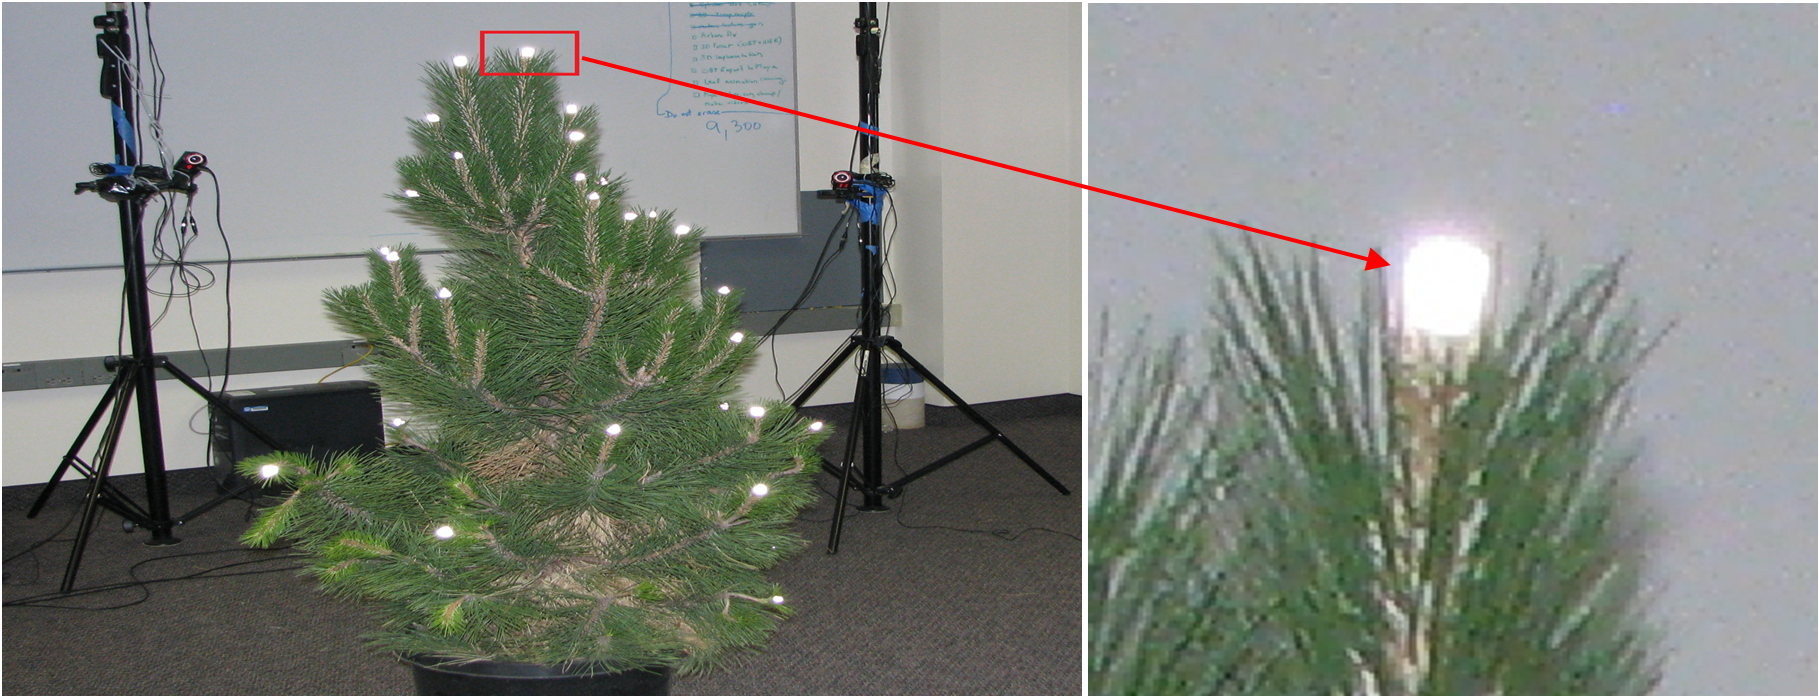
\includegraphics[width=5.0in]{Mocap}
\caption[Marker placement on the crown periphery.]{Marker placement on the crown periphery avoids occlusion while generating data that can be used to generate crown structure.}
\label{fig:mocap}
\end{figure}

Our design requires less user intervention, produces cleaner motion capture data , and may support animation of tree motion.

\section{Data Processing}
\label{sec:Dataprocessing}

Simply inferring positions from one frame of captured data is not adequate due to noise. These branch tips with markers are called "recorded" or "captured" tips. However, the initial locations of recorded branch tips may contain errors due to noise in either the system or the capture environment. 

A clustering algorithm approximates a single initial position from a collection of captured initial positions for recorded branch tips while minimizing error from the motion capture system. The clustering algorithm analyzes positions over many frames of motion capture data and eliminates gaps and noise. Gaps occur when a marker is not present in a frame. This algorithm uses forward differencing to predict a position for a marker at frame $M$ based on positions in previous frames. The closest marker in the next frame is added to the motion trace for the marker if there is a marker located close enough to the predicted position. If there is no marker position recorded close enough to the predicted position, that marker is marked with no data, i.e. a gap, for that frame. Gaps are repaired using interpolation over the motion path for a marker. If the number of marker positions recorded for a marker over time is less than $1/4$ of the total frames, that partial marker trace is marked as noise and eliminated.

If the capture process includes several hundred frames of data in which the tree is not moving, averaging branch tip positions over these frames results in precise estimates of initial positions. In most cases, the number of markers inferred from the clustering process matches the number of markers placed on the tree.

\section{Generating 3D Tree Shape}

Particle flow is a well-studied approach to generating 3D branching structure for trees \cite{Reeves83particlesystems,Runions07,palubicki:siggraph09,neubert:acmtg07}. We adapt the method to motion capture data. The 3D tree crown boundary inferred from motion capture data constrains the particle range and preserves the original 3D tree silhouette. We use a stack of bounding boxes or convex hulls to represent the crown boundary. Particles, either generated randomly in the boundary or locations of branch tips recorded by motion capture, are moving towards trunk nodes. Three forces---gravity, internal force, and external force---drive the particle flow process. The paths of the particle flow produce branching structure. By attaching leaves to the branching structure, we generate a 3D tree model that has similar appearance as the natural tree shape. 

We synthesize a trunk in the center of the crown shape, as shown in Figure \ref{fig:PineTrunk}. Figure \ref{fig:PineTrunksubfig1} shows a photograph of a pine tree with markers placed on its crown. Figure \ref{fig:PineTrunksubfig2} contains a bounding box of these marker locations and a straight vertical line representing trunk shape. The length of the line is scaled by the crown height of the bounding box. On this line segment, we generate about 10 trunk nodes. Random offsets to these nodes in the x and z direction are added as shown in Figure \ref{fig:PineTrunksubfig3}.

\begin{figure}
\centering
        \begin{subfigure}[b]{0.22\textwidth}
                \centering
                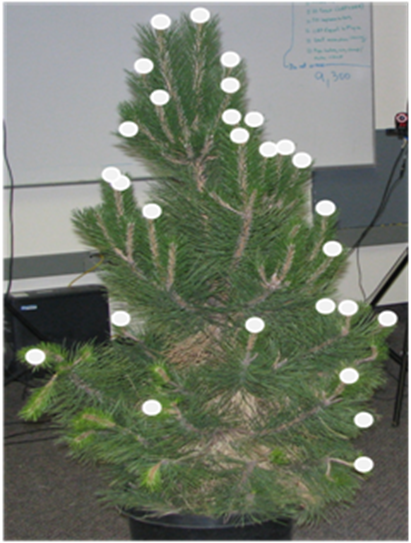
\includegraphics[width=\textwidth]{PineTrunk1}
                \caption{A pine tree with markers.}
                \label{fig:PineTrunksubfig1}
        \end{subfigure}
        ~
        \begin{subfigure}[b]{0.31\textwidth}
                \centering
                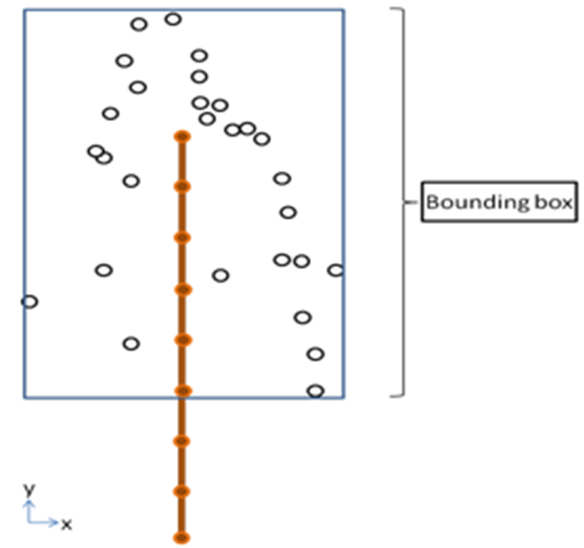
\includegraphics[width=\textwidth]{PineTrunk2}
                \caption{A straight line represents the trunk.}
                \label{fig:PineTrunksubfig2}
        \end{subfigure} 
        ~
        \begin{subfigure}[b]{0.30\textwidth}
                \centering
                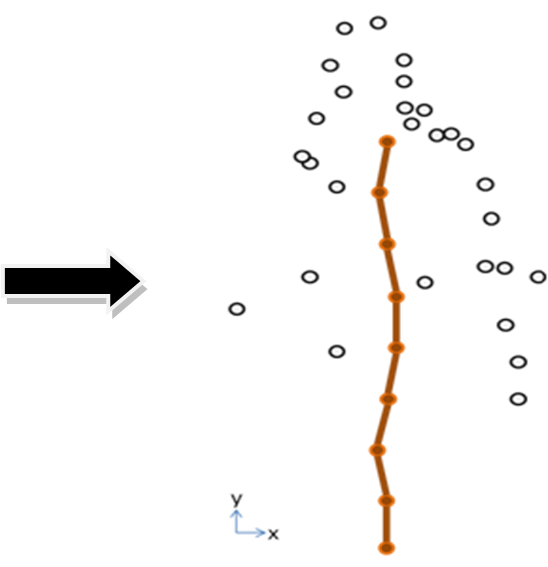
\includegraphics[width=\textwidth]{PineTrunk3}
                \caption{Adding random offsets looks more natural.}
                \label{fig:PineTrunksubfig3}
        \end{subfigure}             
\caption{A simple trunk model is added to the collection of branch tip positions.}
\label{fig:PineTrunk}
\end{figure}

A particle represents a branch tip. One group of particles is 3D positions of branch tips recorded from motion capture, which is described in Section \ref{sec:Dataprocessing}. Figure \ref{fig:PineTrunksubfig1} shows a photograph of a pine tree with markers placed on the crown. All the branch tip locations recorded by motion capture are labeled with white dots. These particles are shown in black circles in Figure \ref{fig:boundboxsubfig3} and Figure \ref{fig:ConvexHullPoints}. 

Because of motion capture's limited capability, we cannot record locations for every branch tip on the tree. Another group of particles is randomly generated within the bounded space of all the recorded branch tip positions. In Figure \ref{fig:boundboxsubfig3} and Figure \ref{fig:ConvexHullPoints}, these particles are green. 

Instead of using one single bounding box for the whole tree crown, we create a vertical stack of bounding boxes as shown in Figure \ref{fig:boundbox}. The new bounding boxes more closely match the tree shape. In Figure \ref{fig:boundboxsubfig3}, the crown height is evenly divided into four parts. Particles are randomly generated inside the smaller bounding boxes, as shown using green dots in Figure \ref{fig:boundboxsubfig3}. The total number of branch tips, including motion capture branch tips and randomly generated particles, is set to be similar to the original tree. The number of green dots in each box is proportional to the number of black dots. Therefore, we maintain a similar total amount and distribution of natural tree branch tips.

\begin{figure}
\centering
        \begin{subfigure}[b]{0.2\textwidth}
                \centering
                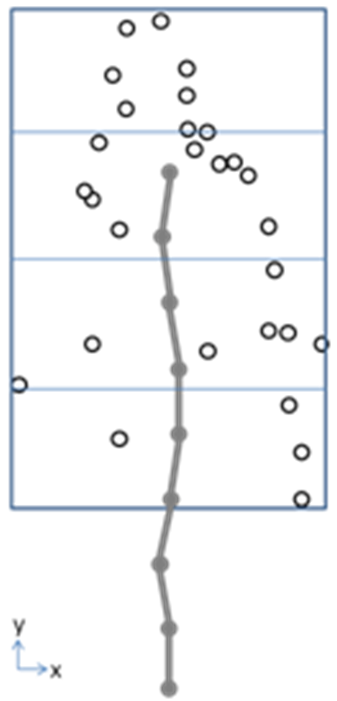
\includegraphics[width=\textwidth]{boundbox1}
                \caption{}
                \label{fig:boundboxsubfig1}
        \end{subfigure}
        ~
        \begin{subfigure}[b]{0.27\textwidth}
                \centering
                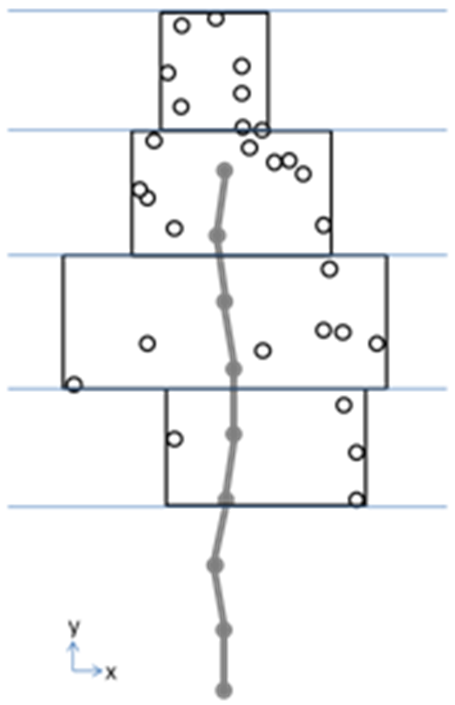
\includegraphics[width=\textwidth]{boundbox2}
                \caption{}
                \label{fig:boundboxsubfig2}
        \end{subfigure} 
        ~
        \begin{subfigure}[b]{0.2\textwidth}
                \centering
                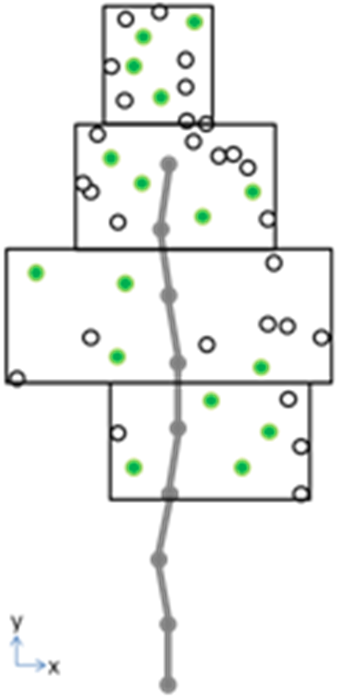
\includegraphics[width=\textwidth]{boundbox3}
                \caption{}
                \label{fig:boundboxsubfig3}
        \end{subfigure}             
\caption{New particles are added within a vertical stack of bounding boxes.}
\label{fig:boundbox}
\end{figure}

Alternatively, we use a convex hull for all the particles, as shown in Figure \ref{fig:ConvexHullPoints}. A convex hull provides more precise bounding space than the stack of bounding boxes. However, it requires a (slightly) more complex boundary detection scheme and more implementation details. Because of the precision that a convex hull brings, we recommend this approach for building a bounding volume.

\begin{figure}[!t]
\centering
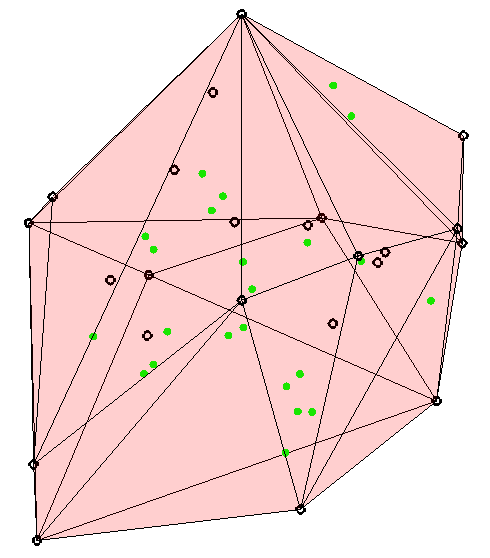
\includegraphics[scale=0.5]{ConvexHullPoints}
\caption[A convex hull for all the particles.]{A convex hull for all the particles. Particles in black color are from motion capture and particles in green color are randomly generated inside the convex hull.}
\label{fig:ConvexHullPoints}
\end{figure}

For the pine tree's trunk, we generate nine nodes in a straight vertical line and add random offsets in the x and z directions to these trunk nodes. The length of the line is scaled about 1.2 times the pine tree's crown height.

Trunk nodes contain a root attractor point and a nearest trunk point, as shown in Figure \ref{fig:flow}. The root attractor point, shown in green, is the trunk node closest to the lower bound of the bounding box for the entire crown. The nearest trunk point, which is shown in blue for the red particle in Figure \ref{fig:flowsubfig1}, is the closest trunk node to a single particle.

\begin{figure}
\centering
        \begin{subfigure}[b]{0.2\textwidth}
                \centering
                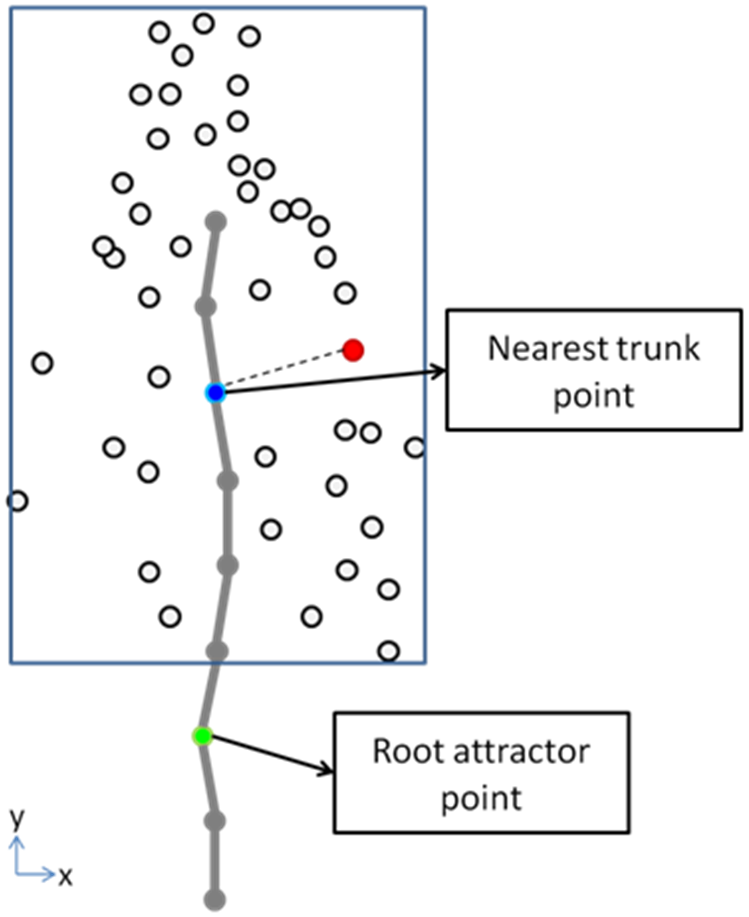
\includegraphics[width=\textwidth]{flow1}
                \caption{Flow direction depends on root attractor and nearest trunk point positions.}
                \label{fig:flowsubfig1}
        \end{subfigure}
        ~
        \begin{subfigure}[b]{0.3\textwidth}
                \centering
                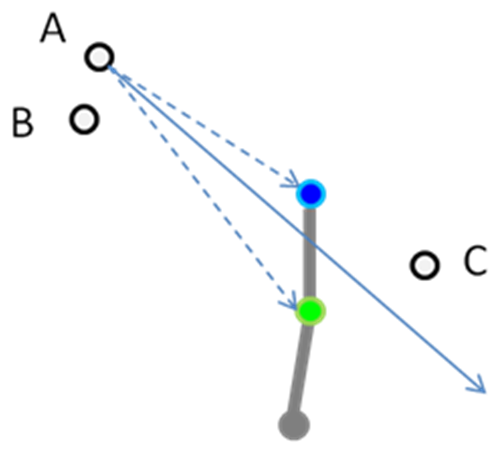
\includegraphics[width=\textwidth]{flow2}
                \caption{Root attractor point $S_r$ and nearest trunk point $S_t$.}
                \label{fig:flowsubfig2}
        \end{subfigure} 
        ~
        \begin{subfigure}[b]{0.3\textwidth}
                \centering
                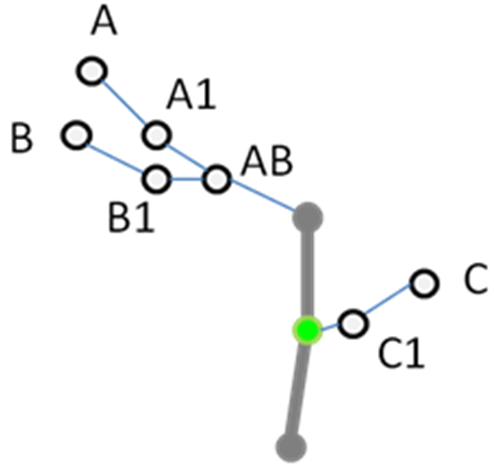
\includegraphics[width=\textwidth]{flow3}
                \caption{Particle flow ends when a particle merges with a neighbor or with the trunk.}
                \label{fig:flowsubfig3}
        \end{subfigure}             
\caption{A simple particle flow results in crown branching structure.}
\label{fig:flow}
\end{figure}

Particles move under directions of three forces: gravity, shape-format, and dominant wind. In Figure \ref{fig:forceTable}, we describe the direction and magnitude of each force. Gravity points vertically down to the ground. We assume that a particle has higher mass when it is closer to the trunk. This assumption follows the observation that when closer to the trunk, a branch has a larger radius. For a particle with higher mass, it has a larger magnitude of gravity and moves faster in the vertical downwards direction. Under this assumption, we set the magnitude of gravity proportional to the distance between a particle position $S_p$ and nearest trunk point $S_t$. 

We call the second force shape-format. Arborists distinguish styles of growth habit of trees using different classifications, such as excurrent and decurrent. The force tries to guide particle flow to follow the growth pattern of the original tree. Simulating different growth patterns requires different definitions of the shape-format force. In this research, we provide a simple example of shape-format definition. The shape-format force, shown in Figure \ref{fig:forceTable}, guides the particle flow process by height and depth of a tree crown. The direction of the force is pointing to the root attractor point $S_r$ from particle location $S_p$. The magnitude of the force is the average height of all the particles with a weight parameter $\alpha$. The higher the center of all the particles, the stronger the shape-format force points to the root attractor point $S_r$. This force is a pre-computed global force, which is a constant for all the particles. The direction of the force ensures that a particle finally merges to trunk nodes, and therefore all the branches grow towards the trunk.

The dominant wind direction is recorded from the motion capture setup, as described in Section \ref{sec:Motioncapturetrees}. Wind force is a special case of external force acting on the tree's branching shapes and structures. While doing motion capture, we record the location of the electrical fan. Because we only use one fan to create wind, that is the only source of explicit external force. Alternatively, the dominant wind direction can be inferred from tree movements recorded in motion capture data. Statistic methods, such as PCA , can estimate the dominate wind direction.

\begin{figure}[!t]
\centering
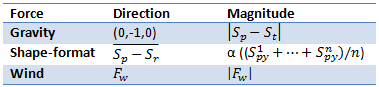
\includegraphics[scale=1.2]{forceTable}
\caption[Definition of three forces. ]{Forces: gravity, shape-format, and dominate wind. 
$S_p$: position of a particle. $S_{py}$ is position of a particle in $y$ direction.
$S_t$: position of the nearest trunk point.
$S_r$: position of the root attractor point.
$F_w$: wind measured from motion capture setup.
$\alpha$: scaling weight in range of [0, 1].
$n$: number of particles.
}
\label{fig:forceTable}
\end{figure}

The flow of particles starts at branch tips. Some particles merge in the flow process while others eventually reach and merge to the trunk. At each time step, we compute for step size and direction of a particle. The step size $L$ is:

\begin{equation}
\label{eqn:model1}
			L = \beta * ||S_p, S_t||,
\end{equation}

where $\beta$ is a tunable parameter in range of [0.1, 0.5] for most of our tree models. The step direction combines all the three forces. Figure \ref{fig:flowsubfig2} shows the computation of the direction for particle $i$, which is shown as particle $A$ in Figure \ref{fig:flowsubfig2}. Each force has a weighting parameter $\omega$ that tunes the relative importance of each vector and provides flexibility in creating branching shapes. The particle step direction $\vec{D_i}$ is given by

\begin{equation}
\label{eqn:model2}
	\vec{D_i} = (\omega_1*\vec{G_i} + \omega_2*\vec{S_i} + \omega_3*\vec{W_i} )/3,
\end{equation}

where $\omega$ is the weight of the direction, $\vec{G_i}$ is direction of gravity, $\vec{S_i}$ is direction of shape-format, and $\vec{W_i}$ is the wind direction for particle $i$ where $i\in[1,...,n]$.

Using step size $L$ and direction $\vec{D}$, the new particle position $V(m)$ is given by

\begin{equation}
\label{eqn:model3}
 V(m) = V(m-1) + L*\vec{D_i},
\end{equation}

where $m$ is current time step and $V(m-1)$ is the particle position at the last time step.

At each time step, after updating all the particle positions, particles might be merged. When the distance between a pair of particles is less than a predefined merging threshold, those particles are combined. When the distance between a particle and a trunk point falls below a predefined merging threshold, that particle is merged with the trunk. In Figure \ref{fig:flowsubfig3}, we demonstrate the paths of particle flow. Particle $A$, $B$, and $C$ are moved using the step and direction. Particle $A$ and $B$ are merged at point $AB$ and finally merged to the trunk. Particle $C$ merged to the trunk point after two time steps of movement.

\section{Adding Leaves}

Tree leaves are visually important to 3D tree models. After the branching structure is generated, leaves are attached. We use predefined leaf shapes, growth patterns, densities, and sizes. Also, because leaves do not always start growing at the beginning of a branch, we set a parameter called the leaf starting point. This parameter is proportional to a branch length. For example, when the parameter is $0.3$, it starts leaves after the point that is $0.3$ times the branch length away from the branch starting point. 

\section{Results}

Results are given for multiple trees, including maple and pine trees. The maple tree is instrumented with 24 markers placed on the periphery of the crown at branch tips and the pine tree is instrumented with 35 markers also located on branch tips. We collect the stationary locations of these markers for about 20 seconds at the capture rate of 100 frames/sec.

Figure \ref{fig:clustersubfig1} shows all the recorded locations as red dots for a single frame, and Figure \ref{fig:clustersubfig2} shows averaged locations from each cluster of marker positions for clusters in which the number of frames with a position in that cluster is $1/4$ of the total frame count. The data is recorded when the tree is stationary. Notice that a point in the blue box in Figure \ref{fig:clustersubfig1} is identified as noise and removed by the clustering algorithm. For the maple tree, after clustering and averaging only 24 markers remain and this matches the actual number of markers placed on the tree.

\begin{figure}
\centering
        \begin{subfigure}[b]{0.4\textwidth}
                \centering
                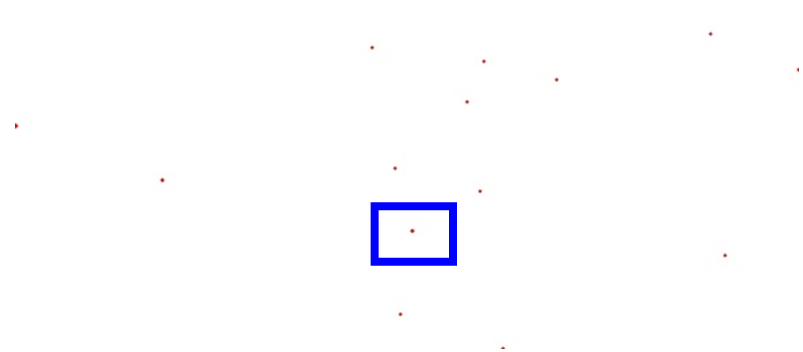
\includegraphics[width=\textwidth]{cluster1}
                \caption{Original collected data.}
                \label{fig:clustersubfig1}
        \end{subfigure}
        ~
        \begin{subfigure}[b]{0.4\textwidth}
                \centering
                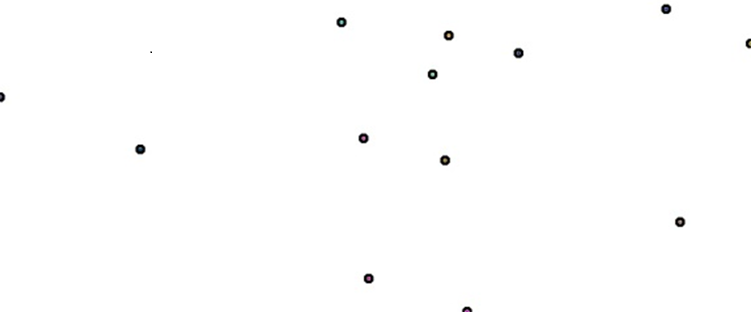
\includegraphics[width=\textwidth]{cluster2}
                \caption{Remaining branch tip locations after clustering.}
                \label{fig:clustersubfig2}
        \end{subfigure}     
        \caption{Clustering that removes noise that leads to spurious marker positions.}
        \label{fig:cluster}
\end{figure}

Although initial marker positions are collected before wind is applied when the tree is stationary, the data contain a small amount of noise, which can be removed to create a single initial marker position. In Figure \ref{fig:markerPath}, we show marker positions over time for two markers during the stationary phase. The horizontal axis shows time while the vertical axis shows a marker location in 3D space. In the first image, movement in each direction spans $10^{-3}$ meters. In addition, in the second image there is apparently a small periodic motion for the stationary branch tip. The range of motion is also within $10^{-3}$ meters. In both cases, averaging removes this small motion and estimates initial marker positions based on the average rather than a single position in a single frame.

\begin{figure}
\centering
        \begin{subfigure}[b]{0.42\textwidth}
                \centering
                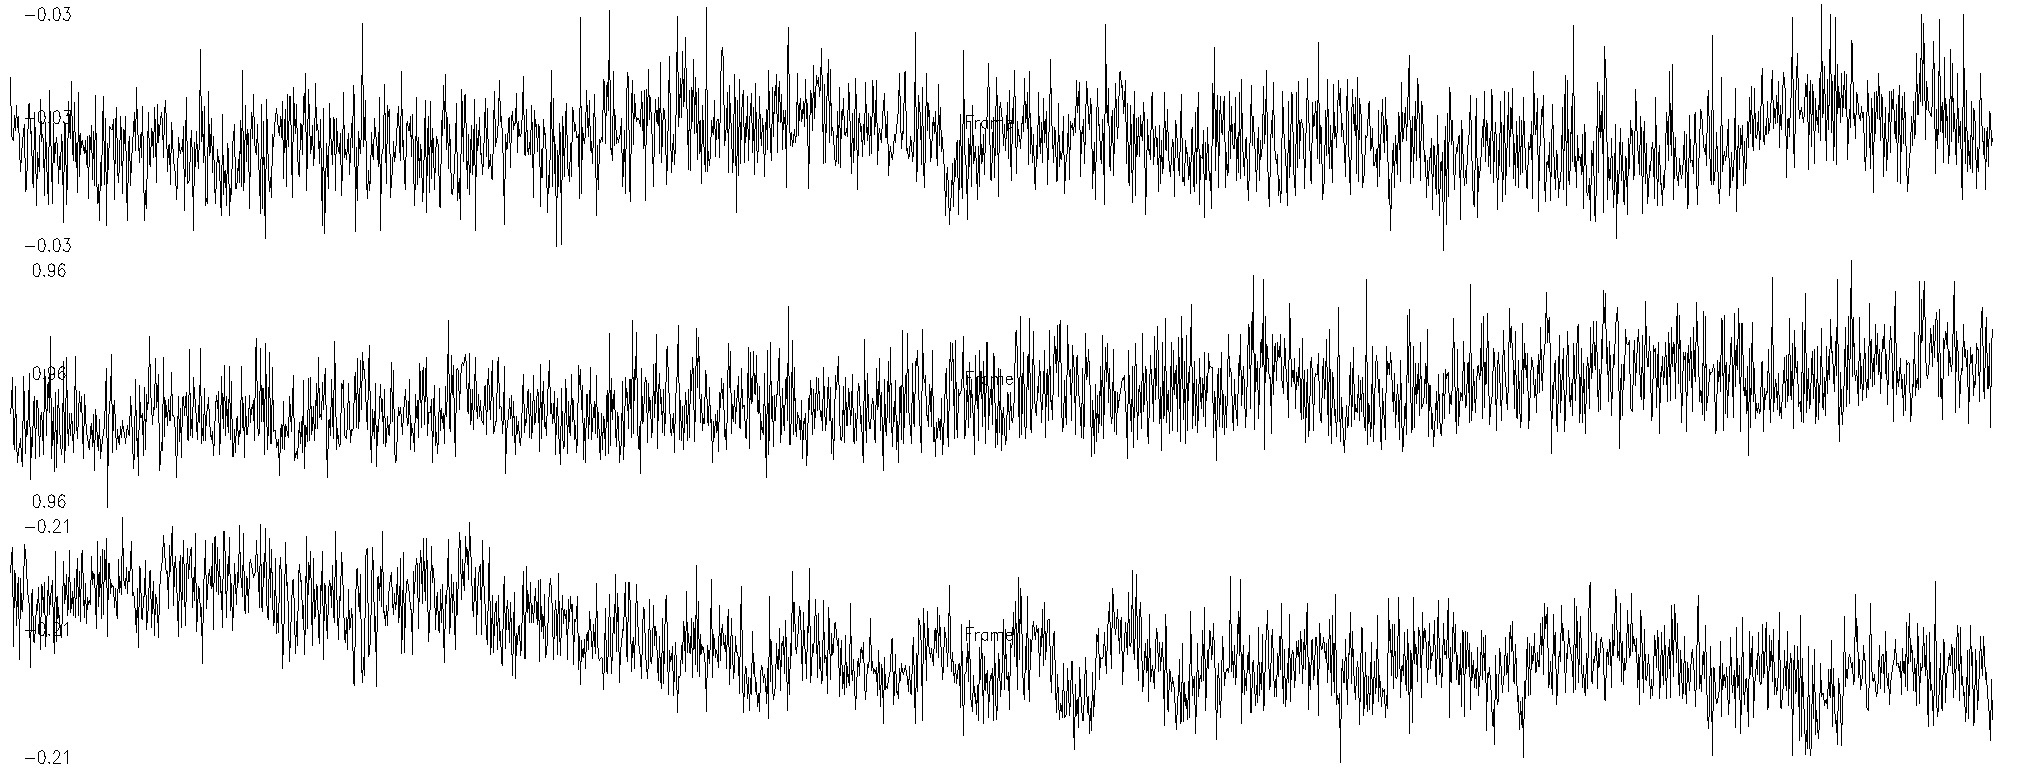
\includegraphics[width=\textwidth]{Marker0orig}
                \caption{Close to white noise.}
                \label{fig:markerPathsubfig1}
        \end{subfigure}
        ~
        \begin{subfigure}[b]{0.42\textwidth}
                \centering
                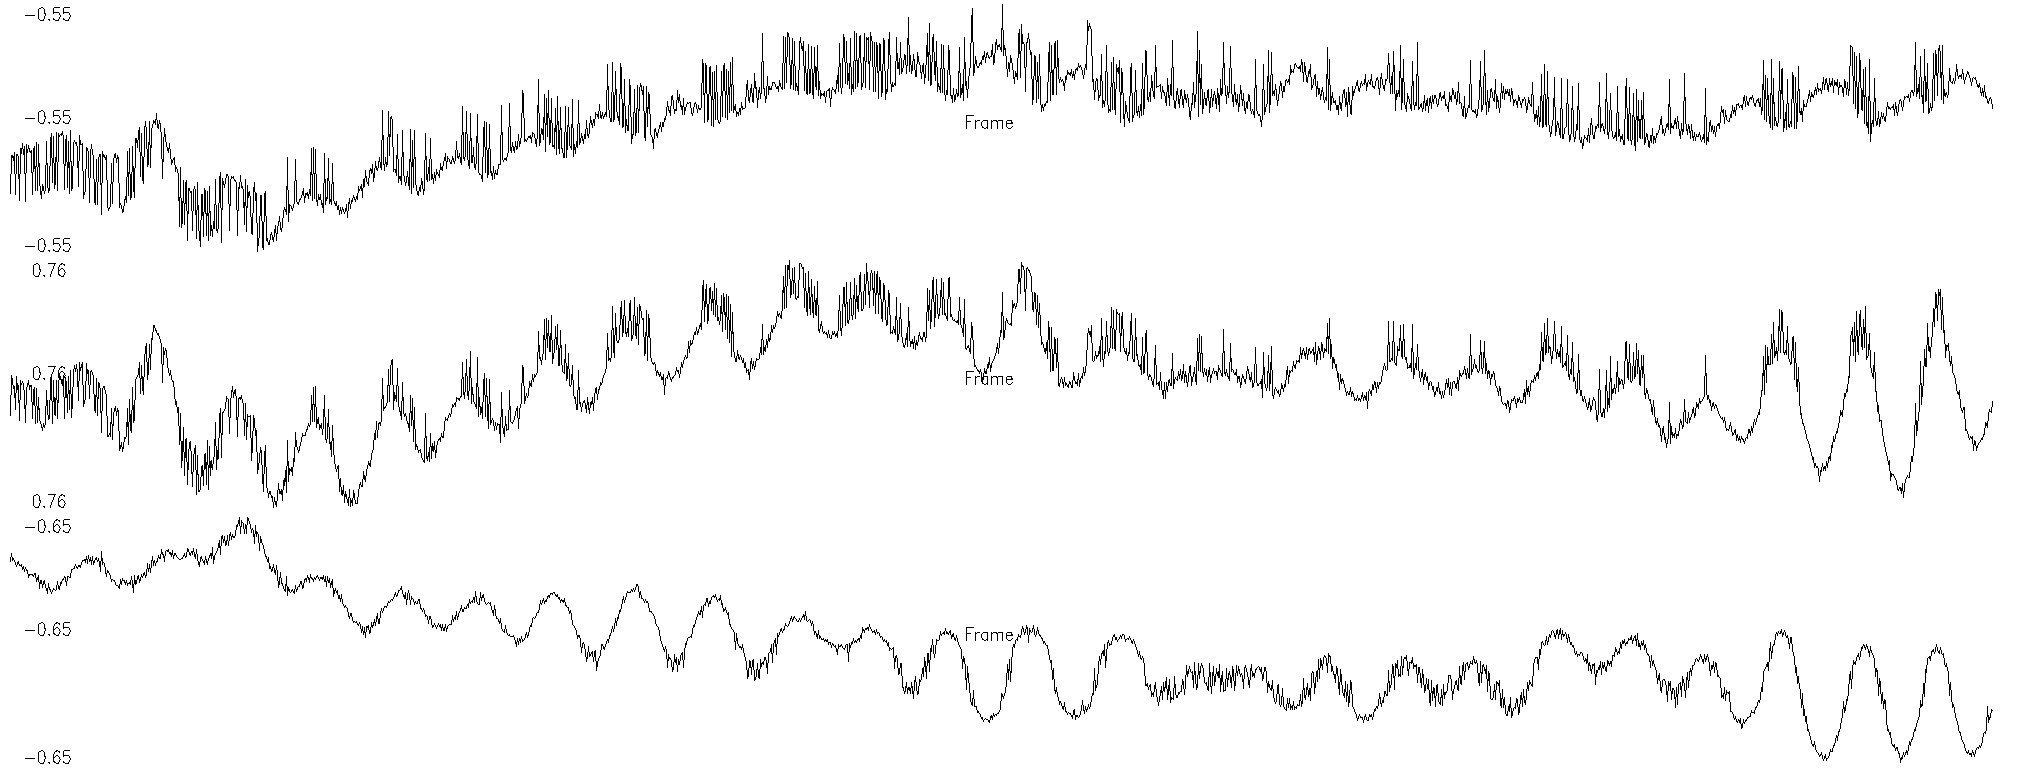
\includegraphics[width=\textwidth]{Marker5orig}
                \caption{Noise with apparent periods.}
                \label{fig:markerPathsubfig2}
        \end{subfigure}     
        \caption[Remove spurious motion. ]{Marker positions over time contain a small amount of spurious motion that is removed by averaging.}
        \label{fig:markerPath}
\end{figure}

A vertical stack of bounding boxes is a better approximation for the crown volume than a single bounding box and results in better crown shapes. Each bounding box contains branch tips and additional branch tips are added to each box. Figure \ref{fig:boundboxsizesubfig1} and Figure \ref{fig:boundboxsizesubfig2} illustrate the difference between tree crowns created with and without a stack of bounding boxes for a pine tree. Random particles placed uniformly within a single bounding box result in a cube shaped tree. Placing particles in a vertical stack of bounding boxes better approximates the original crown shape. Future work might include investigating non-uniform distributions of randomly inserted points instead of using bounding boxes. 

In Figure \ref{fig:boxTree} and Figure \ref{fig:convextTree}, we demonstrate the difference between tree shapes using stacked box bounding volumes and those using convex hull bounding volumes. The bounding box approach provides a looser bounding condition and allows more random factors in the final tree shape. The convex hull approach more closely approximates the original tree crown shape.

\begin{figure}
\centering
        \begin{subfigure}[b]{0.33\textwidth}
                \centering
                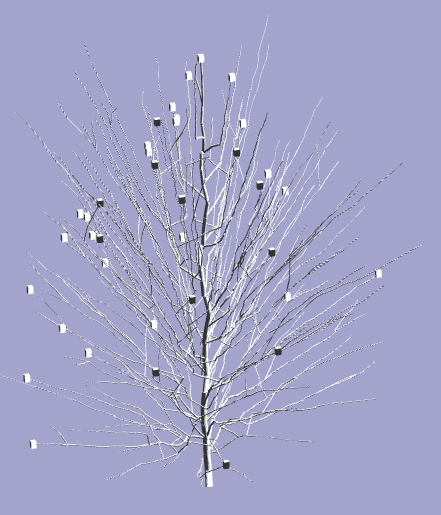
\includegraphics[width=\textwidth]{ResultBoundPine2}
                \caption{}
                \label{fig:boundboxsizesubfig1}
        \end{subfigure}
        ~
        \begin{subfigure}[b]{0.34\textwidth}
                \centering
                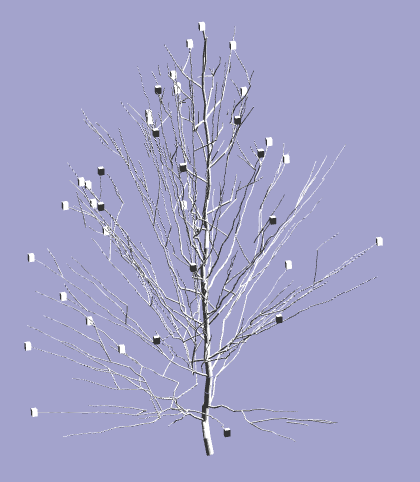
\includegraphics[width=\textwidth]{ResultBoundPine1}
                \caption{}
                \label{fig:boundboxsizesubfig2}
        \end{subfigure}
        ~
        \begin{subfigure}[b]{0.34\textwidth}
                \centering
                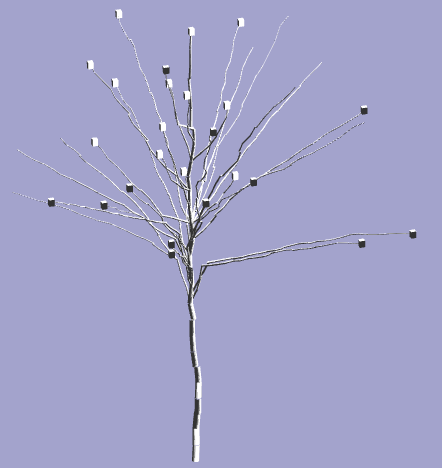
\includegraphics[width=\textwidth]{boundBoxTree}
                \caption{}
                \label{fig:boxTree}
        \end{subfigure}
        ~
        \begin{subfigure}[b]{0.33\textwidth}
				        \centering
				        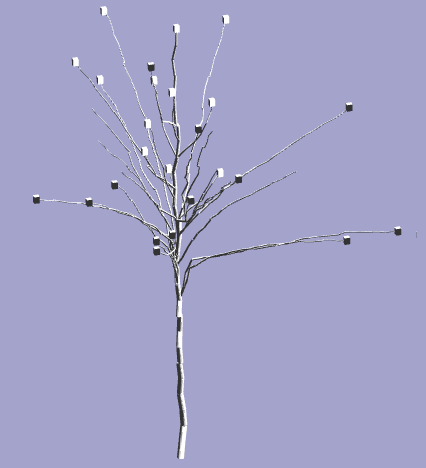
\includegraphics[width=\textwidth]{boundConvexTree}
				        \caption{}
				        \label{fig:convextTree}
        \end{subfigure}
\caption{Bounding volumes affect tree shape.}
\label{fig:boxConvex}
\end{figure}

Particle flow starting from branch tips and using our simplified algorithm results in tree crown shapes that mimic the shape of the tree from which data were collected. In the Figure \ref{fig:treemodelssubfig1}, we show the results from reconstructing a pine tree. 

\begin{figure*}[!t]
\centering
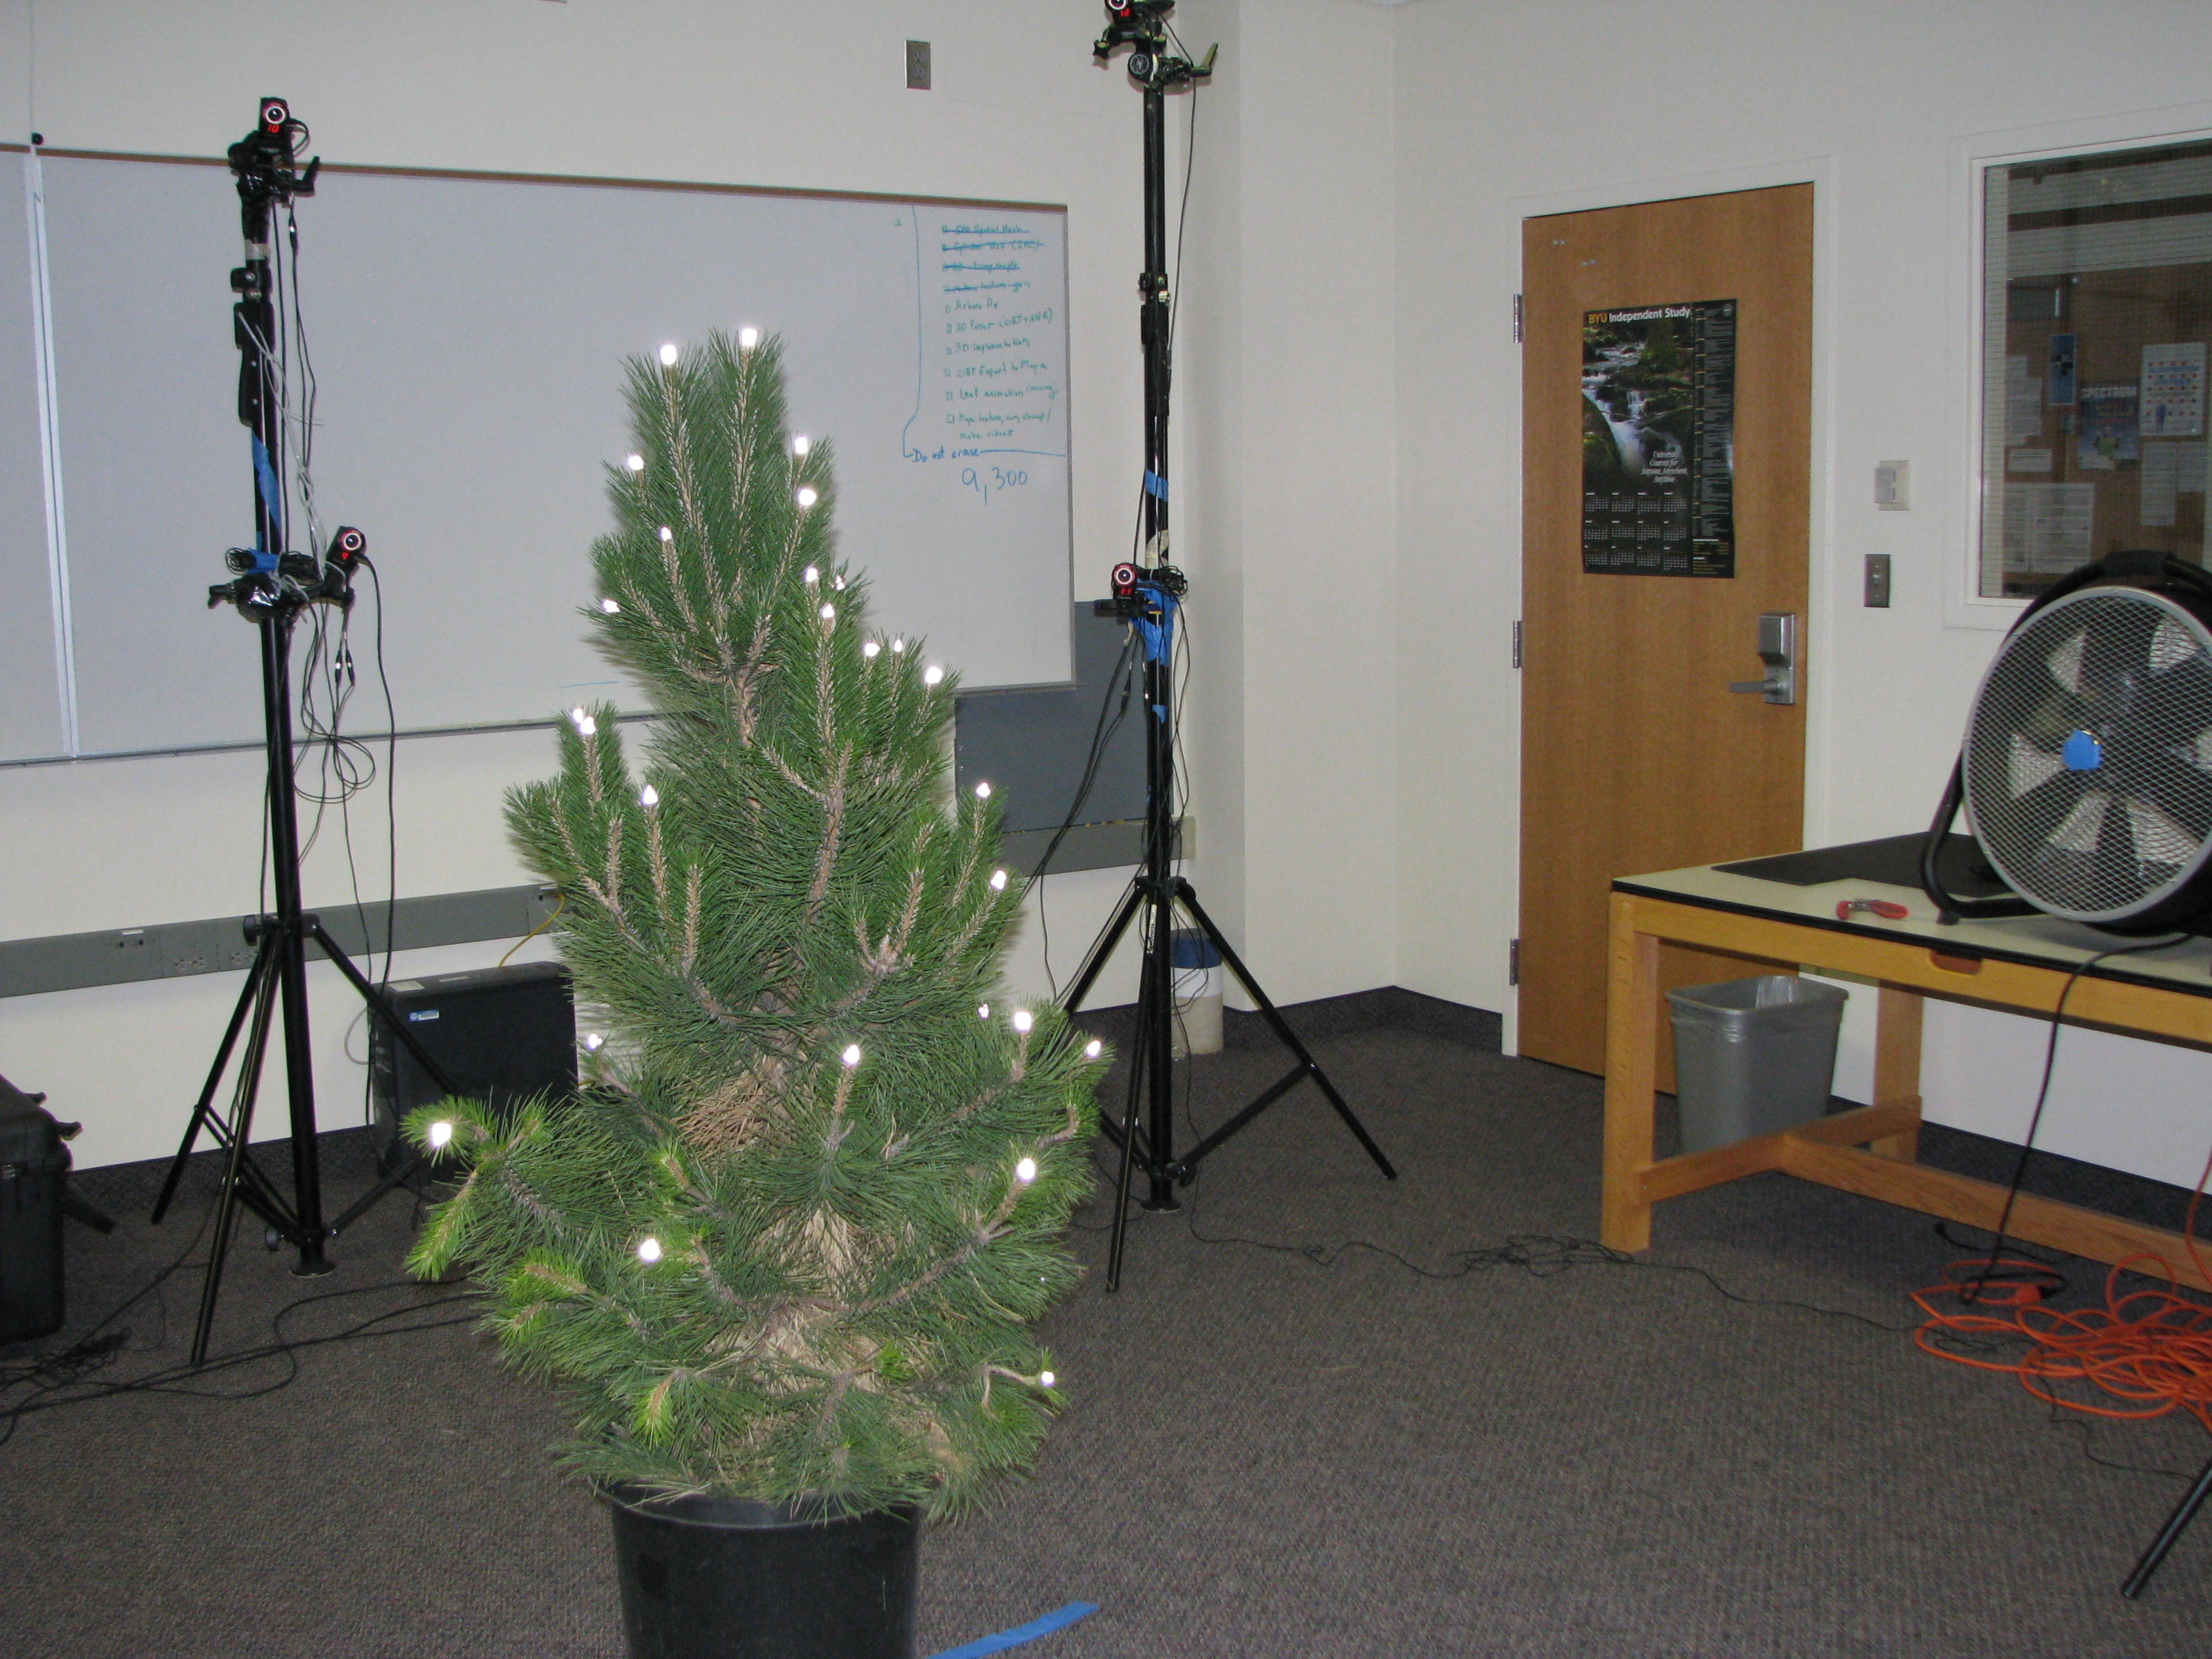
\includegraphics[scale=0.36]{Pine}
\caption[Pine tree model.]{Pine tree model. 3D tree models created from branch tip positions are similar to the shapes of the trees from which branch tip positions were collected.}
\label{fig:treemodelssubfig1}
\end{figure*}

Besides replaying the original tree shape, our approach has enough flexibility to produce different tree shapes based on the same set of motion capture data. Three forces with their scales create particles' moving paths, which represents branching structures. Figure \ref{fig:currency} demonstrates that shape-format force sets the global attracting trunk node, which controls the converging direction of particle flow. The resulting tree models display trees' growth styles in terms of excurrent and decurrent.

\begin{figure}
\centering
        \begin{subfigure}[b]{0.33\textwidth}
                \centering
                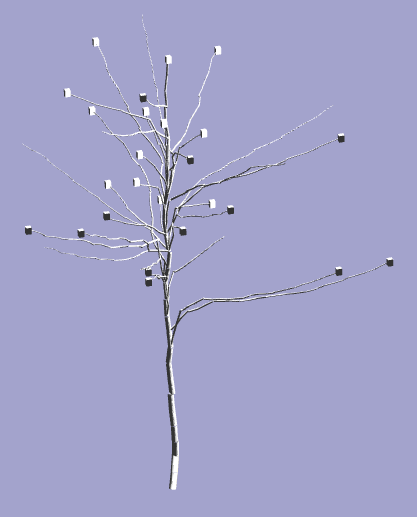
\includegraphics[width=\textwidth]{currency1}
                \caption{}
                \label{fig:currency1}
        \end{subfigure}
        ~
        \begin{subfigure}[b]{0.33\textwidth}
                \centering
                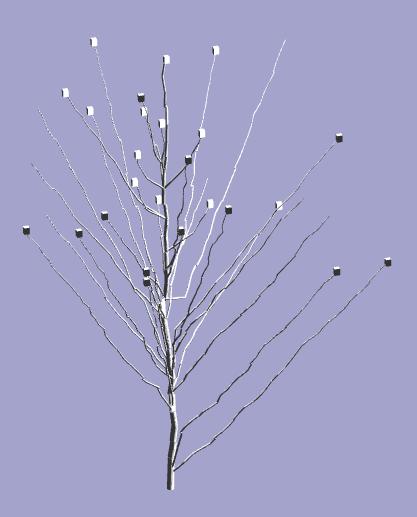
\includegraphics[width=\textwidth]{currency2}
                \caption{}
                \label{fig:currency2}
        \end{subfigure}
\caption{Shape-format force.}
\label{fig:currency}
\end{figure}

Figure \ref{fig:gravityTree} shows the impact of gravity on trees' shapes with various values for the weighting factor. When the factor is set to be negative, we create a special willow-like tree shape. 

\begin{figure}
\centering
        \begin{subfigure}[b]{0.3\textwidth}
                \centering
                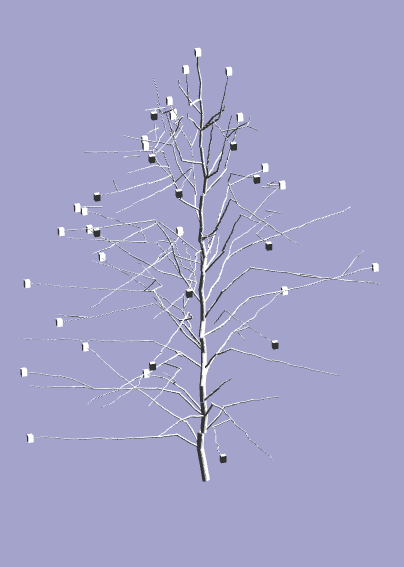
\includegraphics[width=\textwidth]{gravity001}
                \caption{weighting factor: 0.01}
                \label{fig:gravity001}
        \end{subfigure}
        ~
        \begin{subfigure}[b]{0.3\textwidth}
                \centering
                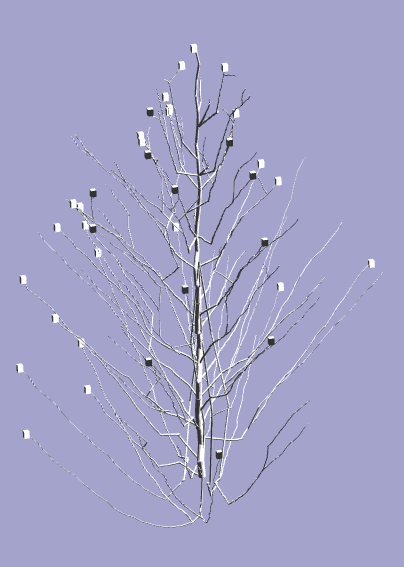
\includegraphics[width=\textwidth]{gravity020}
                \caption{weighting factor: 0.20}
                \label{fig:gravity020}
        \end{subfigure}
        ~
        \begin{subfigure}[b]{0.3\textwidth}
                \centering
                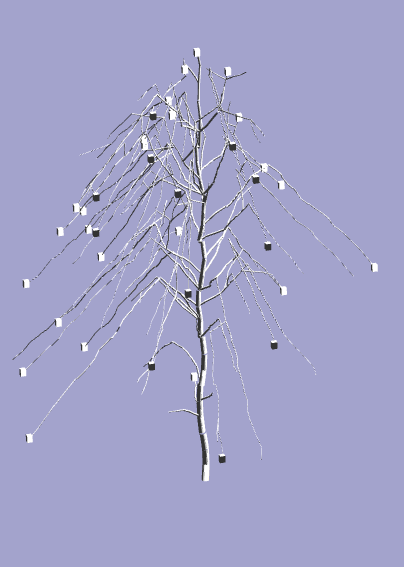
\includegraphics[width=\textwidth]{gravityNeg020}
                \caption{weighting factor: -0.20}
                \label{fig:gravityNeg020}
        \end{subfigure}
\caption{Tree shapes with different weight factors for gravity.}
\label{fig:gravityTree}
\end{figure}

Figure \ref{fig:windFactor} shows tree models with different weighting factors of wind force. Bigger values of the factor produces branches bending more toward the wind direction. Notice that the differences among these tree models are small, especially when compared to the influence from the other two forces. This is because the value of force for a global wind direction is set to be much smaller than that of the other two forces. Otherwise, when wind force dominates the direction of particle movement, the particles might not be able to merge to a tree's trunk and might violate natural tree's shape. 

\begin{figure}
\centering
        \begin{subfigure}[b]{0.3\textwidth}
                \centering
                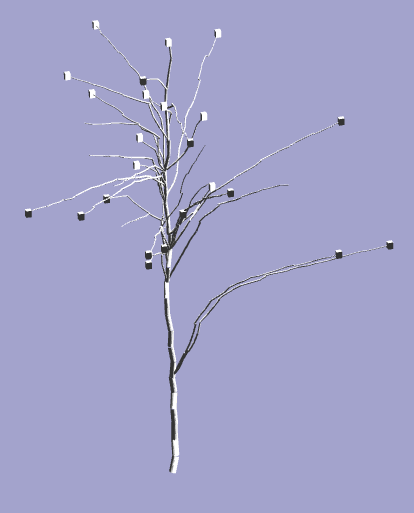
\includegraphics[width=\textwidth]{wind001}
                \caption{Weighting factor: 0.01.}
                \label{fig:wind001}
        \end{subfigure}
        ~
        \begin{subfigure}[b]{0.3\textwidth}
                \centering
                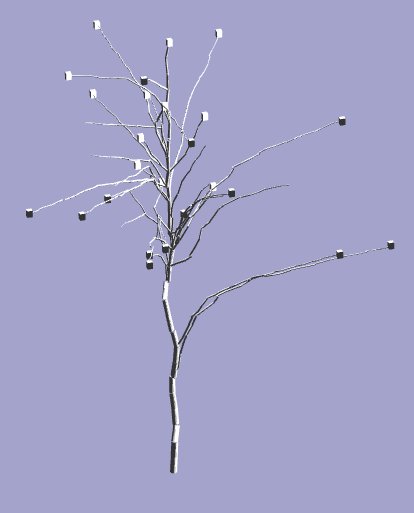
\includegraphics[width=\textwidth]{wind007}
                \caption{Weighting factor: 0.07.}
                \label{fig:wind007}
        \end{subfigure}
        ~
        \begin{subfigure}[b]{0.3\textwidth}
                \centering
                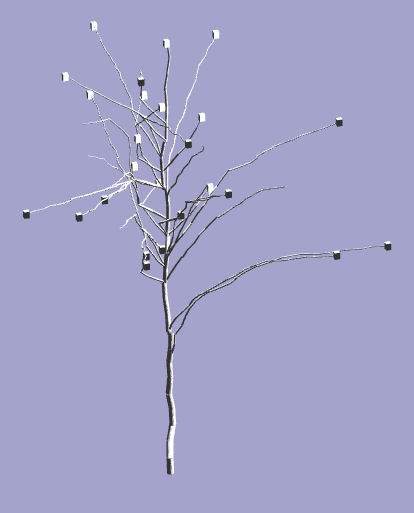
\includegraphics[width=\textwidth]{wind015}
                \caption{Weighting factor: 0.15.}
                \label{fig:wind015}
        \end{subfigure}
\caption{Tree shapes with different weighting factors for wind force.}
\label{fig:windFactor}
\end{figure}

In Figure \ref{fig:moreShapes}, we generate 3D tree models with different parameters for particle flow with the same set of motion capture data. These results demonstrate that our approach produces visually plausible tree shapes, which becomes scalable for more extended shapes through tweaking parameters of the three forces. 

\begin{figure}
\centering
        \begin{subfigure}[b]{0.3\textwidth}
                \centering
                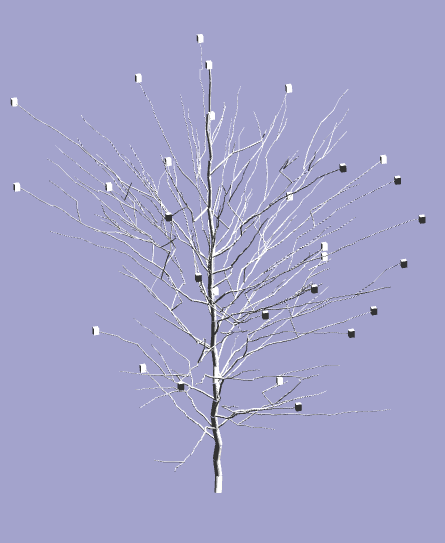
\includegraphics[width=\textwidth]{treediff1}
                \caption{}
                \label{fig:treediff1}
        \end{subfigure}
        ~
        \begin{subfigure}[b]{0.3\textwidth}
                \centering
                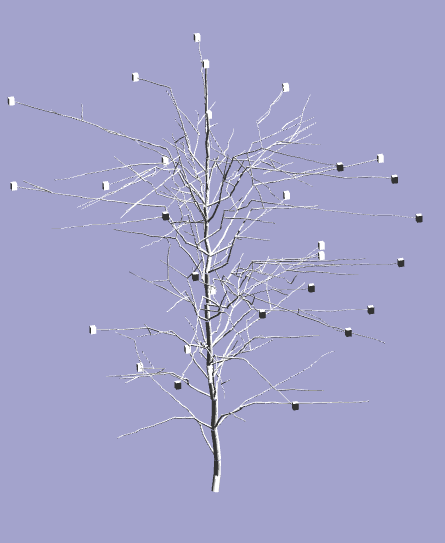
\includegraphics[width=\textwidth]{treediff2}
                \caption{}
                \label{fig:treediff2}
        \end{subfigure}
        ~
        \begin{subfigure}[b]{0.3\textwidth}
                \centering
                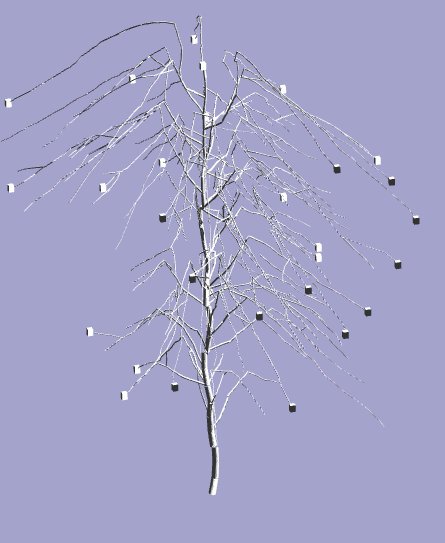
\includegraphics[width=\textwidth]{treediff3}
                \caption{}
                \label{fig:treediff3}
        \end{subfigure}
\caption{Various tree shapes.}
\label{fig:moreShapes}
\end{figure}

\section{Discussion and Future Work}

Placing retroreflective markers on branch tips evenly spaced throughout the crown on trees located in a passive optical motion capture arena results in data that can be used to reconstruct tree shape and which may be usable for replaying branch motion.  This can be done using a simplified particle flow system starting from recorded branch tip positions supplemented with additional random branch tip positions within a horizontal stack of bounding boxes and by setting two control parameters.  A new data collection process designed for trees may extend the use of motion capture to include trees and eventually other networks of non-rigid bodies. 

Future work includes extending the process to large trees outdoors as well as improving methods for animating the resulting tree models using the motion capture data.   We have reconstructed an approximate tree crown branching structure.  Replaying the captured motion data will require care to ensure that the motion of the approximate branching structure does not include uncorrelated motion for branch tips who share a common parent.
\chapter{A Realistic 3D Tree Model Based on L-Systems}
\label{chap:treeLsystem}

\noindent
Jie Long and Michael Jones. \emph{A Realistic 3D Tree Model based on L-Systems. Report for UNEP Eco-Peace Leadership Center (EPLC)}, 2008.

\begin{abstract}
Constructing a 3D tree model manually is time consuming due to the natural complexity of tree shapes. We introduce a new morphology-based method using L-systems for realistic 3D tree modeling. Using L-systems for describing tree branches as particles, this method (1) introduces a hemisphere to generate particles, (2) uses a growth level to simulate different ages of branches, and (3) applies a dynamic bounding box to detect local growth area in a tree. This new method enhances the management of tree shapes by easing the control over distributions of branches and leaves. To further validate the method, we demonstrate that the method can simulate photorealism and growth around physical barriers. We evaluate this model by particle flow and by complexity, showing performance competitive with existing methods.
\end{abstract}

\section{Introduction}

The natural complexity of trees has been challenging computer graphics for decades. Many applications---film, 3D video games, city planning, and forestry---require clear, detailed 3D tree models. Although methods exist for creating photorealistic tree models, these methods are still cumbersome. Efficient methods for constructing 3D tree models are needed to deal with the intractable computation of the detailed geometry. Since trees have many properties due to the growth environment and kinds, models with global controls over shapes are also important. 

In recent years, techniques on image-based reconstruction and L-systems have been widely used in 3D tree modeling research. Both methods have advantages and shortcomings. Image-based reconstruction generates natural-looking 3D trees through image processing, but models are limited to trees in the image and most need time-consuming manual modifications. Although L-systems are efficient and easily implement in 2D or 3D tree models, using L-systems representation alone makes it difficult to control small components in a tree (e.g., a certain twig). 

In this paper, we introduce a new method for 3D tree modeling based on L-systems. This new method presents a 3D tree model with three innovations: a hemisphere, level controls, and a dynamic bounding box. First we build a branch library using L-systems. A branch unit, which is also a unit of L-systems and works as a particle, has several twigs. A hemisphere on the top of a tree model controls the distribution of branches and leaves. The growth levels simulate different ages of branches and leaves. A dynamic bounding box constrains the local growth area in a tree by avoiding outer forces. In the implementation, particles are generated on the hemisphere surface and begin to move in the hemisphere with different starting angles. A ray defined by the position and angle of a particle is attracted to the nearest branch in the existing tree. After a new branch attaches to the existing tree, we enlarge the bounding box to the new tree shape. This bounding box grows with the tree volume and can detect collisions with other objects or growth obstacles. In each growth interval, a certain number of branches are generated and distributed. In addition, leaves have initial parameters for shapes, sizes and colors. We also distribute leaves from the hemisphere surface. In each growth stage, leaves have different sizes and colors, but the same shape. 

There are four steps in this 3D tree modeling. First, L-systems generate different branch patterns. Second, a hemisphere designates probability distributions for generating particles. Third, a branch from the branch library is randomly selected, a particle is generated on the designated area, the ray to the tree model is computed, and the nearest growth point is found.  Finally, after constructing branches for the whole tree, leaves with different sizes and colors are added to this model. 

Using this new method, a 3D tree model is more efficient and controllable. We take advantage of L-systems to describe branches for efficiency while overcoming the control scale problem. L-systems and image-based methods control the whole tree at one time. They generate tree models as a whole. However, our method manages small components of a branch, but not the smallest components of twigs. The second advantage of this new method is the ease of control over tree shape. The hemisphere controls distribution probabilities to shape a tree. The bounding box flexibly constrains a proper growth area to detect outer barriers like rocks and buildings. The parameters of a desired shape are far less than existing methods. In addition, our method can distribute leaves with the same shapes but with flexible sizes and colors due to the growth level of branches. Current methods including L-systems and image-based approaches can't manage the age-based distributions of leaves. Also, we carried out a set of experiments to validate this new method: photokinesis simulation and growth around physical barriers. 

\section{Related Work} 

Two main research directions in tree modeling are biology-based and morphology-based. Models that mimic biological data are based primarily on patterns of tree growth. Some tree modeling software, such as AMAP, COSSYM, and SVS, simulate tree growth based directly on biological data.  Morphology-based methods focus on reconstructing tree shapes from photographs or remote sensing (RS) images. Both biology-based and morphology-based methods have applications in different areas. Forestry research uses biology-based models, and 3D games and movies use morphology-based models.  Our system is mainly morphology-based while also considering some biology characteristics of natural trees. In this section, we discuss two primary morphology-based tree modeling methods: L-systems and image-based models.

\subsection{L-systems}

An L-system is a formal grammar that describes the recursive growth of a tree.  The rules of the grammar must be written by the user. Since the rules are applied locally, small changes in the rules may cause large changes in the overall tree shape. Such behavior makes modeling quite difficult. Various extensions of L-systems have been proposed, including parametric \cite{Prusinkiewicz:sv90}, open \cite{Mech:SIGGRAPH96}, and differential L-systems \cite{prusinkiewicz:siggraph93}. These extensions are able to create a variety of effects, but also require additional parameters from the user. Prusinkiewicz et al. \cite{Prusinkiewicz:2001} present a modeling interface for L-systems to enhance the modeling ease, but a large set of parameters still has to be defined by the user.

L-systems have both advantages and shortcomings. L-systems generate 2D and 3D tree models efficiently. This method is easy to implement. However, L-systems generate tree models at one time after defining an algorithm. Further modification of models is difficult. L-systems go too far in simplifying tree models, so the results are not realistic. 

\subsection{Image Reconstructions}

Reconstruction of tree shapes from photographs is an active area of research in 3D tree modeling. 3D tree models from this method look natural because they are based on the morphology of actual trees. People can use 2D source images, which are easily collected using consumer digital cameras, to generate 3D tree models for almost any interesting trees. 

Shlyakhter et al. \cite{shlyakhter:ieeecga01} direct the growth of L-systems using photographs. The registered input images reconstruct a visual hull. The medial axis diagram of the hull constructs the tree skeleton. L-systems describe smaller branches and leaves. 

Reche Martinez et al. \cite{RecheMartinez2004} describe a very precise, though complex, image-based approach. In this case a set of carefully registered photographs determines the volumetric shape of a given tree. The volume is divided into cells; for each cell a set of textures compute a valid visual representation. The complete set of textures represents the tree quite faithfully. 

Neubert et al. \cite{neubert:acmtg07} present a method to produce 3D tree models from 2D photographs using particle flows. Using image information, the author estimates an approximate voxel-based tree volume. Performing a 3D flow simulation, particles form the twigs and branches. The botanical rules for branch thicknesses and branching angles produce the geometry of the tree skeleton. 

Tan et al. \cite{Tan:2007:ITM} propose an approach for generating 3D tree models from images. This method requires little user intervention. This research populates the tree with leaf replicas from segmented source images to reconstruct the overall tree shape. In addition, shape patterns of visible branches can predict those of obscured branches.

\subsection{Other Methods}

There are some other famous approaches for tree modeling.  Aono et al. \cite{Aono:1984} presented the A-system. Oppenheimer \cite{Oppenheimer1986} proposed the animation based on a fractal method. Reeves \cite{ReevesB85} introduced a modeling method based on particle flow. Reffye et al. \cite{deReffye1988,YAN03} presented a model based on botanical structures. Weber et al. \cite{Weber1998} presented a method on generating trees in several steps. Kurth's team \cite{kurth:sf97} developed LIGNUM \cite{Perttunen98} for 3D tree modeling. 

\section{Tree Modeling Using L-systems} 

Our method has four main parts: a branch library on L-systems, a hemisphere, growth level controls, and a dynamical bounding box. L-systems are easy for describing, controlling, and implementing branch patterns. We can define iterations for each pattern. Users who know L-systems can also define their own branch types easily. The hemisphere controls distribution probabilities for branches and leaves, so we can control tree shapes with a proper randomness. Different growth levels of the tree provide corresponding parameters for both branches and leaves. The dynamical bounding box constrains the local growth area and detects outer growth barriers. 
In a tree model, both local and global characteristics of a tree are considered. Randomly selected L-systems branches control the local shape for every branch. However, we use the probability hemisphere to control the global shape of a tree. 

These four parts work together to produce many tree shapes with efficiency and a natural look. Distribution probabilities for branches and leaves are designated by the hemisphere. This process enables simulations referred to as probability distributions, such as the photokinesis simulation. The bounding box controls local tree shape by detecting outer factors and enables blocked growth. The growth level manages different growth stages for the tree model to decide growth parameters for branches and leaves.

\subsection{Branch Library on L-systems}

L-systems define different branch shapes in our research. Constructing branch shapes is a key problem in simulating 3D trees. Different L-systems algorithms result in different branch patterns. For each branch pattern, we define its rules, angle, and number of iterations. In Figure \ref{fig:eplc1}, we define a branch pattern using a one-iteration L-system (\ref{fig:sub1eplc1}) and show the corresponding branch shape (\ref{fig:sub2eplc1}):

\begin{figure}
\centering
        \begin{subfigure}[b]{0.4\textwidth}
                \centering
                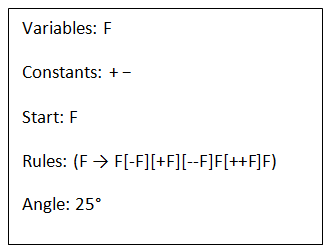
\includegraphics[width=\textwidth]{EPLCfig1a}
                \caption{L-systems algorithms.}
                \label{fig:sub1eplc1}
        \end{subfigure}
        \begin{subfigure}[b]{0.42\textwidth}
                \centering
                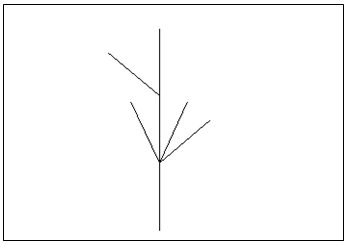
\includegraphics[width=\textwidth]{EPLCfig1b}
                \caption{The corresponding branch.}
                \label{fig:sub2eplc1}
        \end{subfigure}   
        \caption{Tree structure under L-systems.}
        \label{fig:eplc1}
\end{figure}

After giving an L-system for each branch pattern, we use an OpenGL library to draw the corresponding branch. Each fragment (see lines in Figure \ref{fig:sub2eplc1}) of a branch is described by a 3D cylinder. We then apply an angle at the joints to rotate these cylinders. Then we get a 3D branch based on L-systems algorithms. All 3D branches in the branch library have the same length and radius for every twig. When applying a branch to a tree model, we compute the length and radius by parameters from the growth point.

\subsection{Hemisphere for Probabilities Distribution}

A hemisphere controls the distribution of branches and leaves. We define it by a position, a radius, and a probability distribution. The position of this hemisphere is on the top area of a tree model. Its diameter is set by users for different purposes. For example, simulating photokinesis requires the hemisphere to be big enough to include the track of sun movement. The probability distribution divides the hemisphere into several parts and assigns probabilities of particle generation to each part. 

\begin{figure}[!t]
\centering
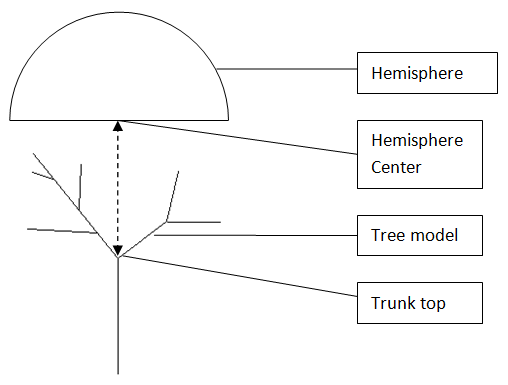
\includegraphics[scale=0.8]{EPLCfig2}
\caption{Side view of a 3D tree model and hemisphere.}
\label{fig:EPLCfig2}
\end{figure}
 
\begin{figure}[!t]
\centering
\includegraphics[scale=0.8]{EPLCfig3}
\caption[An example of probability distribution of hemisphere.]{An example of the probability distribution of a hemisphere (up view).}
\label{fig:EPLCfig3}
\end{figure} 

In Figure \ref{fig:EPLCfig2}, we show the definition of a hemisphere. The size of the hemisphere is bigger than the tree crown. The position is right next to the tree model and the center of the hemisphere is perpendicular to the top of the trunk. 

In Figure \ref{fig:EPLCfig3}, we show an example of hemisphere division and a probability distribution. We cut the hemisphere into several parts. Each part has a specific probability of generating particles. These probabilities control the shape of the 3D tree model.

The functions of the hemisphere have three parts: arranging probabilities for generating particles, defining directions for particles, and setting initial positions for particles. As in Figure \ref{fig:EPLCfig3}, these probabilities decide how particles generate in different parts. In this example, particles are mainly generated in the shaded areas. If the shaded area is the track of the sun's movement, branches in a tree mainly grow towards these areas. When generating a particle on the hemisphere, we first decide the initial position of this particle according to the probability of its region. We then give an initial direction for this particle to move in the 3D scene.

After initializing a particle and its movement in the scene, we define a landing constraint for the particle. The constraint is defined by the user. For example, we can use the nearest Cartesian distance as the constraint. The distance is from the particle's position on the hemisphere to branch top points.

After using the landing constraint to define the landing point on existing tree branches, we select a branch pattern from the L-systems branch library. Using the growth parameters of the landing point, we are able to attach the new branch to the existing tree.

\subsection{Bounding Box for Local Growth Control}

A bounding box defines the minimal 3D rectangular volume around the existing tree model. The bounding box computes the current growth space. When the tree model grows larger, the size of the bounding box grows simultaneously. Therefore, the bounding box can detect whether there are intersections between the bounding box of the tree and other objects. For example, after adding a new branch, if the tree's bounding box intersects with a rock's bounding box, we can delete this branch and generate the next branch.

The bounding box is an approximate method for defining the tree's growth area. In fact, the most exact way is to calculate all points on the tree body. However, this approach is very expensive and not necessary. In contrast, using a bounding box we only need to calculate for two points and detect the growth area approximately. Since a tree has many branches, such approximation highly reduces computations while properly detecting outer barriers.

\subsection{Growth Level Controls}

We introduce the level of growth to control the growth of branches and leaves. In Figure 4, the tree model has three growth levels. Figure 5 shows the corresponding tree model for the growth levels in Figure 4. Because natural trees grow new branches every year, the leaf sizes and colors change according to branch ages and different parts of trees. For example, the color of younger branches and leaves is light green while older ones are dark green or brown. The growth level parameter tracks the age of branches and is used to define leaf and bark appearance. When we add new branches or leaves, the age parameter indicates the right colors, sizes, and other parameters for them. 

\begin{figure}[!t]
\centering
\includegraphics[scale=0.6]{EPLCfig4}
\caption[Various growth levels. ]{Growth level 1, growth level 2, and growth level 3 in a tree model.}
\label{fig:EPLCfig4}
\end{figure}

\begin{figure}[!t]
\centering
\includegraphics[scale=0.8]{EPLCfig5}
\caption{A tree model with three growth levels.}
\label{fig:EPLCfig5}
\end{figure}
 
Growth levels set different particle generations. In Figure \ref{fig:EPLCfig4}, the first generation of particles is the trunk, the oldest part in a tree, having a growth number 1. Then the second generation, branches growing on trunks, has a growth number 2. After adding growth level 3, we get a tree model as shown in Figure \ref{fig:EPLCfig5}. 

Leaves grown in these parts should have darker colors and bigger sizes than those on top, which has a higher growth number. Therefore, different growth levels can simulate different ages of branches and work as a reference for leaves.

\subsection{Tree Generation Steps}

Based on the discussed four parts---L-systems, a hemisphere, a dynamical bounding box, and growth level controls---we can generate a 3D tree model. There are three main steps in this process: (1) define the hemisphere and the branch library, (2) generate particles and control their movements, and (3) distribute the particles in a tree model. We discuss these steps below.

(1)	Define a hemisphere and a branch library.

We define the hemisphere's initial position, size, and probability distribution. The position and size is decided by the scene and the tree size while the center of the hemisphere is identical to the top of the trunk. The probability distribution is defined by users for different purposes. This distribution also reflects the projection of 3D branches on the hemisphere. Therefore, the probability distribution can control the shape of the tree.

As for the branch library based on L-systems, we define different L-systems algorithms and get different patterns of branch shapes.

(2)	Generate particles and control their movements.

We generate a certain number of particles for a growth level at the same time. For example, 10 particles for growth level 2. Then we select proper positions for these particles on the tree.

A particle denotes a branch selected from the branch library. The particle is generated on the surface of the hemisphere according to the probability distribution. With an initial position on the hemisphere and an initial orientation, the particle moves in a Brownian way in the scene.

(3) Distribute the particles in a tree model.

During the Brownian movement, the particle compares and finds a nearest distance among all growth points. Then the branch denoted by this particle is attached to this nearest growth point. After the particle settles, we calculate a new bounding box to replace the old one for this tree. However, there is one exception. After attaching the new branch to the existing tree model, if the new bounding box overlaps some outer blocks, the particle with this branch is cancelled and we then go to the next particle generation. 

After one particle is generated and distributed in a tree model, we repeat step (2) and step (3) until we reach a user-defined numbers of particles. 

\subsection{Examples of 3D Tree Modeling}

Based on this new method with L-systems, we can add more constraints to this model to simulate some properties of natural trees. Here we introduce implementations of trees' photokinesis simulations and of growth control over blocks.

\subsubsection{Trees' Photokinesis Simulations}

The photokinesis simulation relies on the probability distribution on the hemisphere. This simulation is used to make the tree branches grow towards the sun. In order to give more weight to the lighting area, we add more probability of generating tree branches in the track of sun movement. Then the hemisphere works as the sky and the probability distribution is assigned by the sun's track. Figure \ref{fig:EPLCfig6} shows one result of photokinesis simulation.
 
\begin{figure}[!t]
\centering
\includegraphics[scale=0.8]{EPLCfig6}
\caption{A result for photokinesis simulation.}
\label{fig:EPLCfig6}
\end{figure} 

\subsubsection{Growth Control Over Blocks}

We control the growth over blocks by using the dynamic bounding box. When simulating 3D tree growth over blocks, the tree should avoid growing in the blocked area. We use bounding boxes to control blocks, such as outer buildings or rocks. First, we calculate bounding boxes of the blocks. During steps to distribute branches, when a tree's bounding box goes into the bounding boxes of blocks, the current particle is deleted. Thus we can eliminate tree branches grown in the blocked areas.

\subsubsection{Trees' Fruits Simulation}

We can add fruits on a tree using this method. The process of fruits simulation is similar to the leaf attachment. We define the size, shape, and color for fruits. Then we generate particles on the probability hemisphere and distribute the fruits to different growth levels according to the tree model.

\section{Results} 

This new method works well and has some advantages. This model controls the local shape of branches using L-systems and the global shape of trees using the probability hemisphere. Different growth levels approximately simulate the growth process. The bounding box detects outer obstacles. We analyze these characters in detail below. 

\subsection{Growth Probability Control by Hemisphere}

This method introduces a hemisphere control over tree growth by distributing particle probabilities. The tree shape is decided by the predefined probabilities on the surface of this hemisphere. As we use a particle system to control the distributions of branches, the particles' initial sizes and orientations are defined on this hemisphere. Thus, the main shape of a tree is decided and we can use different types of branch patterns to generate the details.
Figure \ref{fig:EPLCfig7} shows two types of hemisphere control on tree shape. In Figure \ref{fig:EPLCfig7}(a), all branches are grown towards the same direction. In Figure \ref{fig:EPLCfig7}(b), there is only one priority growth direction.

\begin{figure}[!t]
\centering
\includegraphics[scale=0.8]{EPLCfig7}
\caption[Branch directions. ]{(a) Branches towards the same direction; (b) branches clustered together for one direction.}
\label{fig:EPLCfig7}
\end{figure}

\subsection{Growth Level Controls}

We introduce a new conception of growth level controls. In this control, we give different growth levels for different branches, leaves, and even fruits with different ages. Branches, leaves, and fruits with the same growth level can share some parameters, such as sizes, colors, and shapes.
In Figure \ref{fig:EPLCfig8}, we show two results for the growth level work. In Figure \ref{fig:EPLCfig8}(a), this tree model has needle-shaped leaves and heart-shaped leaves. It also has small red flowers on the top level. In Figure \ref{fig:EPLCfig8}(b), we add some fruits to this tree model.

\begin{figure}[!t]
\centering
\includegraphics[scale=0.6]{EPLCfig8}
\caption[3D tree models.]{(a) A 3D tree model with different leaf shapes and flowers; (b) A 3D tree model with fruits.}
\label{fig:EPLCfig8}
\end{figure}

\subsection{Growth Control over Small Components}

This new method has advantages in controlling small components in a tree. Compared to the DLA (Diffusion-Limited Aggregation) method \cite{Vicsek1992,Kim2007} for tree modeling, our method reduces computing work by reducing the particles. Using a branch type as a particle rather than assigning a DLA particle for every twig, fewer particles are needed for the same number of twigs in a tree. Since computation for each DLA particle is the same, fewer DLA particles requires less computation. In Figure \ref{fig:EPLCfig9}, we have the same tree shape. If we use traditional DLA in Figure \ref{fig:sub1EPLCfig9}, the circled branch needs three particles to calculate. But in Figure \ref{fig:sub2EPLCfig9}, we calculate one DLA particle for three twigs in one branch unit.
 
\begin{figure}
\centering
        \begin{subfigure}[b]{0.7\textwidth}
                \centering
                \includegraphics[width=\textwidth]{EPLCfig9a}
                \caption{DLA particles.}
                \label{fig:sub1EPLCfig9}
        \end{subfigure}
        \begin{subfigure}[b]{0.7\textwidth}
                \centering
                \includegraphics[width=\textwidth]{EPLCfig9b}
                \caption{Particles in our method.}
                \label{fig:sub2EPLCfig9}
        \end{subfigure}   
        \caption{Particles with tree shape.}
        \label{fig:EPLCfig9}
\end{figure} 

\subsection{Growth Control for Leaves}

Our method provides a new method of leaf simulation, which is difficult for most current methods. Leaf simulation is difficult to achieve by L-systems because L-systems can't control the positions of leaves randomly on branches. Even the popular image-based approaches have difficulties handling leaf simulation. These approaches usually generate branches very well. However, after branch construction, leaves are added randomly and often can't attach to the branches. Our method uses the hemisphere to handle the overall distribution of leaves in a tree, and we apply growth level controls to define leaves with different shapes, sizes, and colors according to the branch properties to which they attach.

This approach is also effective. We only need to change leaf parameters according to the numbers of total growth levels. At a certain growth level, we define the shapes, sizes, and colors for leaves in that level. As for the whole tree, branches have leaves of the same age. In the natural world, that means the old branches have old and big leaves while young branches have young and small leaves in the same shapes.

\subsection{Growth Control by Bounding Box}

Using dynamic bounding boxes in detecting proper positions for DLA particles gives flexible controls over 3D tree models. We generate the DLA particle in the bounding box and find a position in this bounding box. By controlling this bounding box, we can control the growth of the tree. For example, if the current bounding box overlaps a building's bounding box, the current DLA particle should be canceled.

Figure \ref{fig:EPLCfig10} shows an example of tree growth. In this example, the 3D tree model tries to avoid the white box to grow. This process is similar to the process of a tree growing to avoid outer barriers such as bridges or buildings.

\begin{figure}[!t]
\centering
\includegraphics[scale=0.6]{EPLCfig10}
\caption[Simulate tree growth. ]{Trees grow to avoid the white outer box viewed from two different directions.}
\label{fig:EPLCfig10}
\end{figure} 

\subsection{Randomness}

Compared to traditional L-systems, our method generates tree models with more random shapes. Every branch unit carries an L-system algorithm. Because particles control every branch unit, the whole tree doesn't follow any L-systems algorithms. This approach solves artificial iterations from single pure L-system algorithms. In Figure \ref{fig:EPLCfig11}, (a) is a tree model from the combination method and (b) is from a traditional L-systems algorithm. Figure \ref{fig:EPLCfig11}(a) has a random look while (b) has a self-similar character that makes the tree model artificial.

\begin{figure}[!t]
\centering
\includegraphics[scale=0.8]{EPLCfig11}
\caption[3D tree model compared to L-system. ]{(a) Combination method tree; (b) traditional L-systems tree.}
\label{fig:EPLCfig11}
\end{figure} 

Randomness from the DLA method goes too far for tree modeling. As shown in Figure \ref{fig:EPLCfig12}, the shape from (b) might be more curved than is common in trees. Using the combination method, we can reduce the curvature by reducing the number of particles, which stand for L-systems branch units rather than twigs. 

\begin{figure}[!t]
\centering
\includegraphics[scale=0.8]{EPLCfig12}
\caption[3D tree model compared to DLA. ]{(a) Combination method tree; (b) traditional DLA tree.}
\label{fig:EPLCfig12}
\end{figure} 

\section{Conclusions and Discussions} 

We introduce a new method based on L-systems for 3D tree models. In this method, a hemisphere controls probability distributions for branches, leaves, and fruits; growth level controls the distributions for different ages of branches; and a bounding box detects the outer collisions. This new method employs a moving particle for a branch unit, which reduces computation costs of traditional methods like DLA. The hemisphere controls the probability distributions to simulate some natural properties of trees or some special effects. The growth level can manage the internal growth in a tree through age controls. In the tree construction process, the bounding provides an easy and efficient way to control tree growth. Therefore, we can manage the main shapes using the hemisphere while controlling the internal growth through growth level controls. Under these controls, randomness is added by randomly selected tree branches from the L-systems branch library.

The future work in this research may focus on adding more controls over particle movements. We can try to find some more efficient approaches for distributing L-systems branch units. We can also simulate tree animations using this model. Furthermore, we can apply forestry equations to make tree models follow real growth rules.

\section{Practical Application Plan} 

In this paper, we present an innovative method on 3D tree modeling. Tree modeling is a hot research topic in both forestry and computer graphics. This new method with L-systems can produce a user-defined or random 3D tree model. With this tree modeling method, we can control every part in a 3D tree model, including trunks, branches, leaves, flowers, and fruits. For these parts, we can change colors, textures, and shapes very flexibly. The second advantage is about the level control. Based on this control, parts in a tree with different ages look different. The third advantage is the possibility of hemi-sphere control. This is a new method for controlling the shape of a tree by controlling the probable distribution of particles on this hemisphere. Because of the advantages of this new method, it might have three effects: social, political, and economic, which are discussed below.

However, since this new method is currently a basic idea, further work focused on different application areas is need to achieve these goals.

\subsection{Social Effects}

There are two main aspects of this new 3D tree modeling method that have social effects. One is the innovation of this method. Another is the use of this 3D tree model in our society.  

The innovation of this method provides a new method for 3D tree generating. It can help researchers to understand tree modeling and even find better solutions. This new method takes advantage of traditional L-systems and solves the problems with L-systems. We also introduce a new approach using hemisphere and level control. What's more, the bounding box technique can also be applied to this 3D tree model for detecting outer collisions of growth.

This new method can also be used in less technical communities. Based on our idea, we can produce more types of trees and control all parts in a tree. If this method can be applied to work as a demo in some community or school, it helps more people to know how trees grow in a computer. Furthermore, if more biological characters are added, forestry researchers can use this model to predicate the growth of trees and then evaluate the wood productions. However, in addition to our tree model, more work is needed to do to achieve these social effects. 

\subsection{Political Effects}

This model has little effect on politics. However, we suggest this tool for governing trees in a forestry department. At present, most forestry departments use a database or even paper to record and manage trees. With our 3D tree model, we can display these data in visual 3D and thus get more direct information from these data. Therefore, our new method, if there are any political effects, can help forestry departments and researchers to get more information from tree data and help to make some decisions. 

\subsection{Economic Effects}

One reason for the interest in 3D trees is the wide applicability and economic value. As a product of this simulating tool, the automatic generated tree model can reduce manual work and achieve a good simulating result. Our 3D tree model can be used in commercial 3D games, commercial software of tree models, city planning, and so on. 

In commercial 3D games, our tree model can set up a good scene or background. If further work can be done, we will try to improve the efficiency of the current model to make it more applicable.

In commercial software, the method for generating a 3D tree shape is important. Current 3D tree modeling software, such as XFrog, has a great market. Our method suggests a new method of 3D tree modeling and is easy to control. Since this model can also be used in 3D tree modeling software, the method has potential economic value in software design.

In city planning, we can use different shapes of 3D tree models to view corresponding designs. For example, when we choose a type of tree for use on a street, we can generate different 3D tree shapes to make comparisons.
\chapter{Animating Trees Using Wind Fields Estimated from Motion Capture Data} 
\label{chap:estwindfield}

\noindent
Jie Long and Michael Jones. Estimating wind flow from tree motion using motion capture data.

\begin{abstract}
We present non-rigid motion capture by extracting external forces from motion capture data and then replaying those forces to create animation. We explore this idea in the context of motion capture of natural trees in wind.  Motion of a tree in wind is decomposed into three forces: wind-induced drag, branch elasticity, and damping by the leaves.  Given a model of elasticity and damping, the drag force can be isolated and used to estimate wind velocity.  The extracted velocity field is extended to a larger volume and enriched with a turbulence model.  That wind field can be replayed on a tree model that includes elastic and damping properties to create similar motion. 
\end{abstract}

\section{Introduction}

\begin{figure}
\centering
        \begin{subfigure}[b]{0.30\textwidth}
                \centering
                \includegraphics[width=\textwidth]{mocapMaple}
                \caption{Motion capture setup.}
                \label{fig:subfig1}
        \end{subfigure}%
        ~
        \begin{subfigure}[b]{0.3\textwidth}
                \centering
                \includegraphics[width=\textwidth]{simulatedField}
                \caption{Extracted wind field.}
                \label{fig:subfig2}
        \end{subfigure}
        ~
        \begin{subfigure}[b]{0.3\textwidth}
                \centering
                \includegraphics[width=\textwidth]{motionPathMaple}
                \caption{Branch motion paths.}
                \label{fig:subfig3}
        \end{subfigure}        
        \caption[Estimate wind flow and create tree motion. ]{Wind flow can be estimated from motion capture data and used to recreate similar tree motion.}
        \label{fig:title}
\end{figure}

We address the problem of extracting a spatially varying wind velocity field from partial motion captured data and simulating networks of flexible tree branches embedded in a turbulent flow described by this wind field. This problem is a specific instance in which capturing motion and directly replaying it is difficult.  Directly replaying motion capture data is difficult in other settings, such as swimming and rope motion capture, as well.  The problem of replaying tree motion in wind is important for animators and game developers. Tree motion can be an important background element in outdoor settings.  

Animation of trees in wind has been discussed for many years \cite{Akagi:cg06,stams:eu97,shinya:eu92}. In most of the previous research, the wind field is created using noise and fluid simulation. Motion capture avoids the directability and computation problems of simulated wind fields but may yield data that validates simulation-based models.

Motion capture of non-rigid bodies is difficult. Prior work has focused mostly on cloth and facial motion capture \cite{Kwatra:TVCG200966,Ma:FPS2008,SifakisEftychios2005,Lorenzo03}. In these methods, the focus is on overcoming difficulties associated with reconstructing the motion of a deforming plane. We focus on the motion of a deforming network of rods. Rather than directly reconstructing the motion of the deforming object, we reconstruct the forces that create the motion. The forces can then be extended and enhanced to recreate similar motion. 

We solve the problem of extracting a wind field from motion capture data by separating the forces acting on a tree and isolating the force due to wind. There are three primary forces that create tree branch motion: elasticity, damping, and drag. Elasticity and damping can be estimated directly from position and velocity information computed from marker positions. Elastic and damping forces are subtracted from total force to obtain drag. Given drag, we can solve for wind velocity using the aerodynamic drag equation. All of these steps depend on estimates for elasticity, damping, mass, and drag coefficients. These coefficients are estimated from the forestry and graphics literature and can be adjusted to create different motion effects. The extracted wind field has low spatial resolution due to the distances between markers. A sub-grid scale turbulence model with higher resolution restores motion due to omitted high-frequency small-scale turbulence. We use a classical turbulence model composed of a mean flow velocity and turbulence velocity. The mean flow velocity is computed from motion capture data while the turbulence velocity is created using a $tke$ model \cite{Selino:2012,pfa10,pope2000}. The $tke$ turbulence model trains the mean velocity field and modulates tuned noises. By integrating these tuned noises into the wind field, we can restore branches' high-frequency motion while preserving the coherence of branch movements on a tree from large-scale turbulence and small-scale turbulence. 

The process is illustrated in Figure \ref{fig:title}. A tree is instrumented with small retroreflective markers, placed in a passive optical motion capture arena, and subjected to wind. A wind field is extracted, as shown in the middle image. The wind field is applied to a tree model and the resulting motion paths of branch tips are shown in the right-most image.

Our primary contribution is creating complete tree motion from partial motion data collected from motion capture. We discuss methods for sampling and extracting the external force on tree branches as well as energy transformation between tree and wind.

\section{Related Work}

Our work is most closely related to prior work in motion capture of flexible objects and in animating trees. In contrast with prior work in motion capture, we focus on flexible rods rather than flexible planes and on extracting external forces rather than directly extracting motion. In contrast with prior work in animating trees, we estimate a wind field from motion capture data rather than simulating the wind field using noise or approximating it using fluid simulation. 

Motion capture has been widely used in simulating human motion \cite{Kwatra:TVCG200966,Lou:EHM2010,Rajko:2007:RAK,Wen:2006:MCD}. Prior work in motion capture of flexible objects focuses on reconstructing a mesh, which deforms to match a moving surface. Ma et al. \cite{Ma:FPS2008} train a polynomial displacement map and apply this map to create high-resolution facial expressions, including muscle deformation, wrinkles, and skin pores. Lorenzo et al. \cite{Lorenzo03} build a surface-oriented deformation paradigm to animate facial expressions with user intervention. Sifakis et al. \cite{SifakisEftychios2005} combine motion capture data with an anatomical model to produce a model of facial musculature, passive tissue, and the underlying skeletal structure. A key difference between natural trees and facial motion capture is that the drag forces that create natural tree motion in wind may be simpler to extract from motion than the muscular forces involved in facial motion. In this paper, instead of continuously reconstructing a surface, as one does with faces or cloth, we animate trees that have open structures and more degrees of freedom. Also, not only do we create tree motion, but we also simulate wind dynamics, which are scalable.

Recent work extracts forces rather than motion. Kwatra et al. \cite{Kwatra:TVCG200966} simulate human swimming and interaction with water by combining motion capture data and fluid dynamics. Motion capture records swimming motion with an articulated rigid skeleton model. The forces at joints are computed. By combining the forces with fluid dynamics, this method creates human swimming motion as well as water movement. Our research computes wind forces from motion capture data. Compared to Kwatra et al. \cite{Kwatra:TVCG200966}, this would be like capturing the motion of a swimmer in water in order to capture the fluid dynamics around the swimmer. A key difference in our model is that we have assumed that the tree does not initiate motion.

Sun et al. \cite{Sun:2003:VID} propose a method to extract motion patterns from video sequences and reapply these patterns to simulate computer-generated objects. The research focuses on the schema of video input driven animation (VIDA). Motion information is analyzed from 2D video and then incorporated to a conceptual model, such as wind or water dynamics. Our research follows a similar process to the schema. Instead of capturing 2D video, our motion capture system provides more accurate motion information in 3D space. Our research also calculates the interactive energy between trees and wind using particle flow in both space and time domains. By introducing a turbulence model, our tree motion provides more flexibility of simulation control and creates plausible natural tree sway in wind.  

Approaches for simulating tree motion in wind with either one- or two-way coupling in a fluid simulation are based on the Navier-Stokes equations. Akagi \cite{Akagi:cg06} takes this approach but uses a coarse simulation grid, which omits significant high-frequency fluid turbulence. 

The more common approach is to approximate wind dynamics with a frequency-tuned noise model. Ota et al. \cite{ota:cgi03} apply an experimental noise model of ${1/f^\beta}$ to simulate the motion of branches and leaves. Shinya and Fournier \cite{shinya:eu92} present a motion model based on a stochastic process and physical dynamics. They use a power spectrum and autocorrelation of wind to generate a spatiotemporal wind velocity field similar to that created when wind flows through trees. Habel \cite{Habel09PGT} builds a 2D-motion, rather than velocity, texture by combining a Gaussian field with a frequency-tuned 2D velocity field based on a wind dynamics equation with a harmonic oscillator model. The motion texture synthesizes branch motion directly without an integration step. This runs in real time for three moderately complex trees. Stam \cite{stams:eu97} creates filters for white noise and generates wind fields from samplings. He defines and applies the filtering rules in the frequency domain. The noise model with physical dynamics provides control flexibility and works to create motion for complicated large-scale scenes \cite{ZhangSTCP06}. In our research, wind field calculation is driven by branch movements recorded from motion capture. A turbulence model preserves local wind dynamics using particle flow. Using a smooth window, our approach also avoids the complicated time integration of the dynamic system.

Models for simulating large deformation in networks of flexible rods can be applied to animation of trees in wind. Barbic and Zhao \cite{Barbic:2011:RLS} present a scalable method for simulating both internal and external forces that can be applied to trees. If combined with a model of external forces due to wind, this may result in convincing methods for animating trees in wind.  

Tree motion can also be simulated using data from video or motion capture. Diener \cite{Diener:2006} records 2D video and extracts features for a single plant. By analyzing the video with these features using hierarchical retargeting algorithms, the 2D motion is projected into 3D space and animates a large class of virtual shrubs.  Long et al. \cite{Long:MCN2010} reconstruct 3D tree motion in wind using motion capture. Reflective sensor markers are placed along branches. Leaves have to be sparse to ensure the visibility of all markers exposed to capture motion. This approach produces visually realistic movements of a cherry tree in wind. However, this method can only create motion of the original tree and is not scalable to other models. In our research, wind field information is trained from motion capture data. Using particle flows for local wind energy transfer, we are able to simulate the motion of multiple objects in a scene. In addition, reflective markers are placed on the tree crown instead of along a single branch. This design maximizes the visibility of markers to motion capture and records more accurate movement data. It also facilitates the computation with the dynamic model of wind and tree.

\section{Methods}

We estimate a wind field from tree motion using motion capture data.  Natural tree motion is captured using passive optical motion capture.  The data are analyzed to estimate both a 3D model of the tree geometry and a wind field.  The estimated wind field approximates the wind that created the motion recorded in the motion capture data.  A fluid simulation enriched with a synthetic turbulence model transfers energy between wind and tree.  The enriched fluid simulation drives animation of a tree model.  

Our work can be divided into three parts: motion capture, tree modeling, and wind--tree interaction. We describe each part in the following sections. Of those three parts, wind--tree interaction presents the most difficult and interesting problems. 

\subsection{Motion Capture}

As in \cite{Long:MCN2010}, twelve optical motion capture cameras are placed in a circle around a tree indoors. A fan with varying speed and direction creates tree movement. The cameras record the motion of markers placed on exterior branch tips. Placing markers on branch tips avoids problems with occlusion. Typically we use about 30--70 markers, depending on the size and shape of the tree. Markers are distributed evenly to cover the crown shape. 

Optical motion capture records unindexed locations of all the reflective markers in a scene. The recorded data can be processed to label unindexed locations and to eliminate swaps and repair gaps. The algorithm uses forward differences to predict the future position of a point and then minimize the distance between the predicted and the recorded points to add a new position to an existing trace. Details can be found in \cite{Long:MCN2010}. At the end of the process, collected marker positions are clustered into paths for each marker. 

\subsection{Tree Modeling}

Particle flow can generate 3D branching structures \cite{Tan:2007:ITM,neubert:acmtg07,Runions07}. In most cases, this approach depends on inverse volumetric rendering to identify the position of tree mass.  The tree mass is then filled with a branching structure using either particle flow or pre-built libraries of small branching structures.  Motion capture data simplify the process because explicit image segmentation and camera calibration are not needed, as they are part of the motion capture process.  

Particle systems generate the branching structure.  In our process, particles are generated at the 3D positions recorded for the branch tips on which reflective markers were placed. We generate additional particles distributed evenly on the periphery of the region bounded by the tree crown. Each of these particles also represents a branch tip.

\begin{figure}[!t]
\centering
\includegraphics[width=1.8in]{particle}
\caption{A particle with its nearest trunk point and its crown root point.}
\label{fig:particle}
\end{figure}

The particles flow toward a predefined trunk placed vertically in the center of the crown shape. Branch shapes and hierarchies are defined when particle paths connect. Particle flow starts at branch tips and ends at the trunk. Each particle has a direction, a step length, and a threshold for merging. As in \cite{neubert:acmtg07}, the particle direction combines the direction to the crown root point and to the nearest trunk point, shown in Figure \ref{fig:particle}. The red dots in the image indicate locations of branch tips. The crown root point is the lowest point on the trunk near the bounding box of tree crown. The nearest trunk point is on the trunk that has the shortest distance toward a particle. Particles flow from branch tip toward the trunk, which is unlike the particle system in \cite{palubicki:siggraph09}, where particles flow from trunk to branch tip. The direction of the first step in the flow is the combination of direction to the nearest trunk point and the crown root point. In the following steps, the flow direction is also a combination of these two directions, but any two particles are merged if their distance is under the threshold of merging distance.

\subsection{Wind--tree Interaction}

Wind--tree interaction is based on a mixed Lagrangian/Eulerian model of the wind field extracted from motion capture data enriched with a subgrid turbulence model. The Eulerian grid stores wind velocities as estimated from motion capture data. Lagrangian particles carry velocity and turbulent kinetic energy $tke$ from frame to frame. The \textit{velocity grid} is replaced every frame while the \textit{fluid particles} retain state from frame to frame.
Fluid particles carry energy back and forth between the global wind field, the local turbulence model, and the tree. In this way we simulate tree movement as well as the distribution of energy in a dynamic wind velocity field.

Proxy geometry is used to detect and approximate the effects of collisions between fluid particles and tree geometry. Both the effect of wind on trees and the effect of the tree on wind are calculated.  

Because the global velocity field is generated from motion capture data, which may contain noise, this field may not be continuous in the time domain. Averaging velocity values for a single grid across several adjacent frames smoothes these variations but also smoothes small-scale turbulence effects. In order to compensate for lost turbulence effects as well as to better preserve wind continuity over time, particles store $tke$ across frames and manipulate the scale of turbulence due to characteristics of tree and wind. 

\subsubsection{Wind Velocity Field}

The global grid-based velocity field is the source of wind energy in the scene. Wind force is estimated directly from recorded displacements of branch tips. We solve for wind velocity at branch tips using drag equations and the estimated wind force.  This gives a sparse collection of velocity estimates.  Interpolation and extrapolation build a grid of velocity values from the sparse collection. Figure \ref{fig:vectorField} shows an orthographic projection of such a field. The green dots indicate marker positions, the red arrows represent extracted wind velocities, and the blue arrows represent velocities interpolated or extrapolated from the estimated velocities. The wind field in Figure~\ref{fig:vectorField} is quite smooth.  This is because small-scale turbulent eddies are below the spatial sampling resolution of the motion capture data.  A subgrid turbulence model based on $tke$ recreates small eddies in the velocity field. 

\begin{figure}[!t]
\centering
\includegraphics[width=2.5in]{vectorField}
\caption{Vector field of wind velocities with estimated and interpolated values. Wind velocity estimates based on recorded tree motion are shown in red with interpolated velocities in blue.}
\label{fig:vectorField}
\end{figure}

We isolate the drag force in order to estimate the wind velocity.  Assuming no external forces other than wind influence the tree motion, the motion of a branch is caused by aerodynamic drag and internal elasticity and damping forces. Elastic forces tend to restore the branch to a resting position and damping forces reduce velocity. In this model, the forces acting on a tree are given by 

\begin{equation}
\label{eqn:1}  
			F = F_{wind} + F_{elastic} + F_{damping} = F_{wind} + c\dot{s} + ks.
\end{equation} 

Differences between marker positions in successive frames give estimates for position $s$, velocity $\dot{s}$ and acceleration $\ddot{s}$. All the derivatives are approximated with the marker positions using backward differencing. The displacement $s$, velocity $\dot{s}$ and acceleration $\ddot{s}$ are calculated as

\begin{equation}
\label{eqn:diff}
s^t = q^t - q^{t-1},\\
\dot{s}^t =  (s^t - s^{t-1})/2.0,\\
\ddot{s}^t = (\dot{s}^t - \dot{s}^{t-1})/2.0,
\end{equation}
where $q^t$ is a marker position at time $t$. The elastic force $F_{elastic}$ is the product of branch elasticity and displacement from the rest position. Similarly, the damping force is the product of the damping coefficient and the velocity. We estimate damping $c$ and spring coefficients $k$ from biomechanical parameters. Since $F = m\ddot{s}$, we substitute $m\ddot{s}$ for $F$, make similar substitutions for the elastic and damping forces, and then solve for $F_{wind}$ to obtain 

\begin{equation}
\label{eqn:2}
			F_{wind} = m\ddot{s} - c\dot{s} - ks.      
\end{equation}

The drag equation gives the force created by wind as a function of the wind velocity $V$ (and other constant parameters explained below): 

\begin{equation}
\label{eqn:3}
			F_{wind} = 0.5\rho(V^2)AC_D,
\end{equation}
where $\rho$ is air density, $V$ is wind velocity relative to branch movement, $A$ is the aerodynamic cross section, and $C_D$ is the drag coefficient.

Substituting the value of $F_{wind}$ calculated using equation (\ref{eqn:2}) into equation (\ref{eqn:3}) and solving for $V^2$ gives

\begin{equation}
\label{eqn:4}
		V = \frac{F_{wind}}{\left\|F_{wind}\right\|} * \sqrt{\left|\frac{m\ddot{s} - c\dot{s} - ks}{0.5{\rho}AC_D}\right|}.
\end{equation}

The solution is based on the assumption that the acceleration is constant and therefore the direction of velocity $V$ and force $F_{wind}$ is preserved as the same in a short period of time. In our case, the time interval is 0.01 sec from motion capture setup. The direction of the velocity $V$ is computed using the unit normal vector of $F_{wind}$ as shown in equation (\ref{eqn:4}). The displacement $s$, velocity $\dot{s}$ and acceleration $\ddot{s}$ are computed using equation (\ref{eqn:diff}) from the marker locations.

The equation (\ref{eqn:4}) calculates a wind velocity estimate in each frame at the location of each branch tip.  Motion capture markers are distributed evenly through the crown in order to sample the global wind field over a large area. 

Interpolating and extrapolating velocity values over the entire motion capture volume results in a grid-based velocity field. The size of a grid cell is set to be close to the average distance traversed by a single marked branch. By doing this, we can optimize the usage of motion capture data during the interpolating and extrapolating process. In each frame, the ideal case is that each grid cell contains exactly one motion-captured point. In our case, the grid resolution is $10*10*10$. We use linear interpolation to fill the grid from sampled values because linear interpolation is simple.  More sophisticated methods, such as Kriging (as in \cite{ganz:cvpr09}) or distance-weighted kernel-based methods, could also be used.

The grid-based wind velocity field is computed from each individual frame of branch tip data. However, the wind velocity field does not vary smoothly from frame to frame because there are gaps and jumps in the data. To improve temporal continuity, velocity values over the neighboring 5 frames are averaged. 

Turbulent motion below the sampling scale of the motion capture data cannot be captured by this model. In space, we are only able to extract turbulent effects that are large enough to influence the motion of two adjacent markers. Because leaves have small mass and large surface area, small-scale turbulence results in visually significant motion on tree crowns. That turbulence is well below the sampling limit of the data. The mean flow inferred from motion capture data will be enriched with a turbulence model at a finer resolution. 

Rather than apply the velocity field directly to the tree, we introduce particles into the field and collide particles with proxy spheres attached to the tree. These particles have zero mass and do not affect the mean flow. This scheme simplifies calculation of wind--tree interaction by replacing cell--tree collisions with point--sphere collisions. Cell--tree collisions can be expensive for determining what fraction of a cell contains a fraction of a generalized cylinder representing the tree branch. With particles and proxy geometry, estimating wind velocity can be reduced to a distance-weighted average of the particles contained in a sphere. 

\subsubsection{Wind Effects on a Tree}
%why we use the approach? motivation
Simulating wind effects on a tree creates branch motion. The simulation is the key to creating natural tree motion. We have discussed creating a grid-based wind velocity field using motion capture data. Because of motion capture's capability to record a limited number of markers, the resolution of the gird is low. The low resolution simulates big-scale turbulence but lacks small-scale turbulence information due to a high-frequency wind field. Selino and Jones \cite{Selino:2012} solve this problem by introducing the small-scale turbulence, which is computed from large-scale turbulence. This solution fits into our problem very well. In our case, the low resolution of the wind velocity field produces large-scale turbulence. The large-scale turbulence will be tuned by a $tke$ model to create small-scale turbulence. The combination produces wind effects, including both large- and small-scale turbulence, on a tree.

% a summary of the approach. 
The simulation of wind effects on a tree preserves coherence of velocity from several perspectives. The mean flow velocity computed from interpolating motion capture data contains information of tree movements as a whole. The $tke$ model keeps track of turbulence changes in the flow and thus tunes the noise value due to these changes. The Gaussian noise field is filtered in the frequency domain to match the frequency of turbulence observed in tree crowns. The model is derived from a classical turbulence model and generates turbulence effects, including both large scale and small scale.

%How does our method work?
Our approach is different from Selino's work because of the source of large-scale turbulence. Instead of a real-time fluid simulation, we generate the large-scale turbulence offline from motion capture. In Figure \ref{fig:turbulenceFlow}, we demonstrate our turbulence model to generate tree motion. The turbulence is computed in two parts as in large scale and small scale. The large-scale turbulence is created from the grid-based wind velocity field. The small scale is generated from the $tke$ model. After solving the turbulence velocity, we apply a drag equation as shown in equation (\ref{eqn:3}) to solve for the tree motion represented by branch displacements. 

\begin{figure}[!t]
\centering
\includegraphics[width=3.4in]{turbulenceFlow}
\caption{Turbulence simulation to create branch motion.}
\label{fig:turbulenceFlow}
\end{figure}

% the basic equation
The turbulence velocity $V(t)$ applied to a branch segment is computed as in equation (\ref{eqn:5}):

\begin{equation}
\label{eqn:5}
		V(t) = v(t)+ \alpha\sqrt{k(t)}N(t),
\end{equation}
where $v(t)$ is the mean flow velocity for the large-scale turbulence at time $t$, $\alpha$ is a tunable weight parameter, $k(t)$ is from $tke$ model, and $N(t)$ is a sampled value from a frequency-tuned time-varying noise field. 

%explain $tke$ tuned high frequency velocity component
In the simulation, each fluid particle carries a mean flow velocity from the global wind velocity field and a $tke$ estimate from the turbulence model. The value $k(t)$ of the $tke$ is estimated using a two-equation $tke$ budget based on strain in the velocity field as shown in equation (\ref{eqn:tkeProduction}) and (\ref{eqn:tkeProductionZero}). The $tke$ model is adapted from Selino \cite{Selino:2012} and Pfaff et al. \cite{pfa10}, and is based on Pope \cite{pope2000}. The value $k(t)$ represents turbulent kinetic energy and is generated when the strain in the mean flow velocity is not zero. The decay term $\epsilon$ models dissipation rate of that turbulence energy. When the turbulence production $P$ exists due to strain, the $k$ and $\epsilon$ are computed as follows:

\begin{equation}
\label{eqn:tkeProduction}
		\frac{\partial{k}}{\partial{t}}=P-\epsilon, 
		\frac{\partial{\epsilon}}{\partial{t}}=C_{\epsilon1}\frac{P\epsilon}{k}-C_{\epsilon2}\frac{\epsilon^2}{k},
\end{equation}
where $P$ is the production of turbulence, $t$ is current time step, and model constants are $\epsilon1$ = 1.44 and $\epsilon2$ = 1.92. When the production $P$ of turbulence in the fluid becomes zero, the values of $k$ and $\epsilon$ dissipate and compute as in the equation (\ref{eqn:tkeProductionZero}):

\begin{equation}
\label{eqn:tkeProductionZero}
	k(t) = k_0\left(\frac{t}{t_0}\right)^{-n}, 
	\epsilon(t) = \epsilon_0\left(\frac{t}{t_0}\right)^{-(n+1)},
\end{equation}
where $t$ is current time step, $n$ is a constant decay component computed by $\frac{1}{C_{\epsilon2-1}}$, $k_0$ and $\epsilon_0$ are the most current values, respectively, in the past when there exists turbulence production $P$, and the reference time $t_0$ is computed as $n\frac{k_0}{\epsilon_0}$.

Based on equation (\ref{eqn:tkeProduction}) and (\ref{eqn:tkeProductionZero}), we compute for the value of $k(t)$ in equation (\ref{eqn:5}).

The noise $N(t)$ is sampled from a continuous noise field. That noise field is tuned to match the frequency distribution of turbulent flow through trees given in Simiu \cite{simiu1996wind}.

%explain mean flow velocity
The mean flow velocity $v(t)$ is sampled using a distance-weighted average of particles' velocity contained within the proxy sphere of a branch tip. Proxy geometry is defined for each branch segment using 3D spheres with radii proportional to branch segment length and diameter as suggested from Selino and Jones \cite{Selino:2012}. 

% a bigger picture
Figure \ref{fig:flowChart} shows the energy flow during the simulation. Wind energy is transferred from the grid-based velocity field to particles. The turbulence model calculates $tke$ from the transferred wind energy. When particles pass through proxy geometry, velocity is converted to a drag force using equation (\ref{eqn:3}) and branch motion is created. 

\begin{figure*}[!t]
\centering
\includegraphics[width=6in]{energyFlow}
\caption{Energy flow in a wind velocity field.}
\label{fig:flowChart}
\end{figure*}

\subsubsection{Tree Effects on Wind}

Tree effects on wind are split into local and global effects. Local effects happen at the scale of a few leaves and branch segments.  Global effects happen at the scale of the entire tree.  Local effects are simulated using a simple damping model on wind particles, and global effects are recorded during motion capture.  Simulating local effects allows for variations in wind flow due to differences between the shape and dynamics of the animated tree compared to the shape and dynamics of the actual tree used in motion capture. 

Tree effects on wind on the local scale are calculated as a damping force for particles within the proxy geometry representation of tree mass. Consider the velocity $v_i(t)$ of particle $i$ in frame $t$  sampled before calculating branch movement. Suppose that particle $i$ lies in proxy geometry for some branch in frame $t$. After displacement of the branch tip has been calculated, if the particle lies within the proxy geometry then we compute the influence of the branch on the particle velocity. The new velocity of particles in the proxy geometry is computed as follows in equation (\ref{eqn:6}):

\begin{equation}
\label{eqn:6}
		v_i^{'}(t) = v_i(t)(1-\beta),
\end{equation}
where $\beta$ is a constant decay rate that changes particle velocity based on damping by the tree. The rate is constant for each branch, but varies due to the size, material, leaf shapes, and other properties of the tree. We set the reduction rate between 0.02 and 0.05 in most simulations. This reduction smoothes out the mean velocity over time while the high-frequency details are compensated from the $tke$ turbulence model.

In the next frame $t+1$, we first load the estimated global grid-based wind field generated from motion capture data. The particle velocity $v_i^{'}(t)$ from the previous frame is used as the mean flow velocity to compute the current particle's turbulent kinetic energy $k(t+1)$. Then we use equation (\ref{eqn:4}) to calculate wind velocity $V(t+1)$ experienced by the tree geometry. 

The global effect of the tree on the wind is inferred from the motion capture data. Branches on the leeward side of the tree have less motion. When the particle exits the proxy geometry, the damping is no longer computed, so the particle velocity is reset to match the estimated global velocity $v$.

\subsubsection{Tree Animation}

The movement of the whole tree is computed from the drag force at each branch tip. We use a damped mass-spring model to define branch dynamics. When the density, stiffness, and damping coefficients match the estimates used to calculate wind velocity, the resulting motion is similar to the original motion. The drag forces are calculated for each branch segment.

\section{Results}
\label{sec:4results}

We present results that show animation of a tree in wind using a wind velocity field inferred from motion capture data for a similarly sized tree moving in wind.  

We first create a 3D tree shape using particle flow. In Figure \ref{fig:treeshape}, the small white cubes on some of the branch tips indicate the location and total number of reflective markers we capture for the tree. The locations of branch tips that do not correspond to a marker location are created within the stacked bounding boxes. We generate tree leaves based on the branching structure and instance leaf size and shape randomly. By the refined bounding box method, the generated 3D tree shape also is visually similar to the crown shape of the original tree. The similarity between the generated tree model and the actual tree shape can be seen in parts (a) and (b) of Figure~\ref{fig:title}.  It is significant that the tree shape does not perfectly match the original tree shape.  Applying the motion capture data indirectly as an inferred wind velocity field, rather than directly as a set of motions, allows for variations in tree shape and branching structure.  

\begin{figure}[!t]
\centering
\includegraphics[scale=0.5]{mapleModelMocapTip}
\caption{3D branching structure with marker locations.}
\label{fig:treeshape}
\end{figure}

The $tke$ model is a significant part of producing realistic motion. In Figure \ref{fig:branchPath}, we compare the results generated with and without turbulent $tke$. Each figure shows motion paths from an animation of a tree in wind with and without sub-grid turbulence based on the $tke$ model.  The path on the left includes motion due to sub-grid $tke$ and the path on the right does not.  In both cases, moving branches trace out arcs of similar size as they sway left and right.  Adding $tke$ has the effect of adding variation to each sway motion so that the arcs are each in a slightly different location.  As a result, the motion path on the left, which includes $tke$, is less compact while the motion path on the right, which does not include $tke$, contains many overlapping arcs.

\begin{figure}[!t]
\centering
\includegraphics[scale=0.6]{branchPath}
\caption[Branch motion paths with and without subgrid turbulence.]{Branch motion paths with (left) and without (right) sub-grid turbulence. Adding turbulence adds small variations to each branch sway, as seen in the less compact motion path on the left.}
\label{fig:branchPath}
\end{figure}

The images in Figure \ref{fig:motionPaths}\subref{fig:branchTipMocap} and \ref{fig:motionPaths}\subref{fig:branchtipSynthesized} compare recorded motion of a tree with motion generated for a similar tree using the wind field inferred from motion capture data.  The actual tree motion is shown using green traces on the left and the generated motion is shown on the right.  Note that motion is not captured for every branch tip on the left, but motion is generated for every branch tip on the right.  The images have been aligned so that the wind direction is the same in both cases.  Branches in similar positions on the crown have similar motion. 

\begin{figure}
\centering
        \begin{subfigure}[b]{0.29\textwidth}
                \centering
                \includegraphics[width=\textwidth]{branchTipMocap}
                \caption{Original tree motion.}
                \label{fig:branchTipMocap}
        \end{subfigure}%
        ~
        \begin{subfigure}[b]{0.3\textwidth}
                \centering
                \includegraphics[width=\textwidth]{branchtipSynthesized}
                \caption{Animated tree motion.}
                \label{fig:branchtipSynthesized}
        \end{subfigure}       
        \caption[Motion paths for the animated tree. ]{Motion paths for the animated tree are similar to motion paths in the original tree for branch tips at the same relative crown location.}
        \label{fig:motionPaths}
\end{figure}

In Figure \ref{fig:mapleSway}, we demonstrate that our method produces plausible tree sway motion and results in tree motion effects observed in nature, such as sheltering.  Branches bend with the wind and then return to their rest position.  Branch sheltering within a single tree crown occurs when branches on the leeward side of the crown experience lower wind velocities than branches on the windward side because drag exerted by the windward branches reduces the wind velocity.  In the figure, the dominant wind direction is from left to right and from the lower left corner. We can observe that branches, which are on the left side (the windward side), have bigger amplitude of motion than others. Besides completing tree motion of a single similar tree with partial motion capture data, our method can also be extended to create tree motion for multiple trees using the wind field.  The trees in Figure \ref{fig:multipleTrees} move in the same wind field.  Although this creates the appearance of a group of trees moving in a shared environment, wind is not damped as it passes from one tree to another.  In the video clip attached to this paper, we provide a side-by-side comparison of the video originally recorded during the motion capturing process and the synthesized tree animation. From the video, we can observe that sheltering effects among branches are successfully simulated. 

\begin{figure*}[!t]
\centering
\includegraphics[scale=0.65]{mapleSway}
\caption[Maple animation.]{Several frames from the animation of a maple tree in a wind field extracted from motion capture data.}
\label{fig:mapleSway}
\end{figure*}

\begin{figure}[!t]
\centering
\includegraphics[scale=0.68]{multipleTrees}
\caption[Multiple trees swaying. ]{Multiple trees swaying in wind field estimated from the motion of a single tree.}
\label{fig:multipleTrees}
\end{figure}

\section{Discussion and Future Work}

We have presented animation of non-rigid bodies using partial motion capture data by extracting a wind velocity field rather than replaying motion data directly. This simplifies the problem as we no longer need to match motion capture data to a precise reconstruction of the original capture subject. It also results in complete and coherent motion from incomplete data that contains discontinuous motion. We have also presented a method for enriching the extracted force field to include fine-resolution turbulence. This is possible because the extracted velocity field can be analyzed and enriched, much like position graphs can be analyzed and enriched in other applications.  

This work opens a new direction in the motion capture of non-rigid bodies in spatially smooth force fields. We have investigated this idea in the context of trees and wind. Future work might focus on other objects, such as cloth, in other flows.

\chapter{Discussion and Conclusion}

The research builds a new model of motion capture for non-rigid bodies under external forces. From partially recorded movements on non-rigid subjects, we create complete animations of these or similar subjects using physical and statistical models. We present a generic pipeline for capturing movements of non-rigid bodies using passive optical motion capture. We have demonstrated animation of non-rigid bodies using partial motion capture data by extracting external forces rather than replaying motion data directly. The approach simplifies the problem as we no longer need to match motion capture data to a precise reconstruction of the original capture subject. It also results in complete and coherent motion from incomplete data that contain discontinuous motion.

Chapter \ref{chap:pilottree} reconstructs tree motion under natural wind. It builds a plausible tree skeleton using a minimal spanning tree algorithm over a cost function defined using position and motion data. Gaps and errors in motion capture data for trees are replaced with data interpolated from neighboring branch motion. These are important steps toward realizing motion capture of trees for tree animation in games. We had hoped to get better results with the repaired data and the rigid body algorithm we used. Based on the results of this pilot project, we believe that investigating other approaches to processing the point cloud are more promising than repairing the errors caused by using the rigid body algorithm we used. 

In Chapter \ref{chap:rope}, our work produces visually plausible rope motion from passive optical motion capture data using a statistical model under the assumption that the rope does not stretch. The algorithm preserves continuity of motion in traces and fits the shape of rope.  This work lays a foundation for further investigation of motion capture for non-rigid bodies using statistical rather than physical models. The approach to the problem may advance motion capture results for non-rigid bodies driven by complex or poorly understood physical systems.

Chapter \ref{chap:treeparticles} generates a 3D tree model using particle flow along with motion capture data. The particle flow system starts from recorded branch tip positions supplemented with additional random branch tip positions within a horizontal stack of bounding boxes and by setting two control parameters. A new data collection process designed for trees may extend the use of motion capture to include trees and, eventually, other networks of non-rigid bodies. 

Chapter \ref{chap:treeLsystem} introduces a new method based on L-systems for 3D tree modeling. This new method employs a moving particle for a branch unit, which reduces computation time compared to diffusion-limited aggregation. We control the main crown shapes with the hemisphere while controlling the internal growth structure using growth levels. Under these controls, randomness is added by randomly selecting tree branches from the L-systems branch library. By introducing the random factors, it is difficult to produce the exact shape of the original tree. Also, small changes in parameters might produce big changes in the output tree shape, which is a common problem when employing L-systems.

Chapter \ref{chap:estwindfield} is based on all of the previous work in our research. In this project, we present animation of non-rigid bodies using partial motion capture data by extracting a wind velocity field rather than replaying motion data directly. This simplifies the problem as we no longer need to match motion capture data to a precise reconstruction of the original capture subject. It also results in complete and coherent motion from incomplete data that contains discontinuous motion. We have also presented a method for enriching the extracted force field to include fine-resolution turbulence. This is possible because the extracted velocity field can be analyzed and enriched, much like position graphs can be analyzed and enriched in other applications. This work opens a new direction in the motion capture of non-rigid bodies in spatially smooth force fields. We have investigated this idea in the context of trees and wind. Future work might focus on other objects, such as cloth, in other flows. We can also extend the process to larger trees outdoors.

As inferred from the rope reconstruction project, complicated motions (such as spirals, collisions, sudden changes in movement, or extremely fast movement) are not well handled in our model. Our assumptions for detecting swaps may be oversimplified relative to natural movement. In the future, consideration of other factors, such as velocity or acceleration, might improve gap-filling results. We have used a simple method for interpolating rope position between markers.  More complex methods may result in more plausible results, particularly when the distance between markers on the rope is large.

Our research discusses animating non-rigid bodies using motion capture, but mostly focuses on replaying motion for trees and ropes. We present a general application of motion capture for non-rigid bodies, including a data collection process and data cleaning algorithms. The work can be extended to non-rigid bodies other than trees and ropes. By emphasizing different non-rigid subjects under various force fields, followed by our general application of motion capture, the data cleaning algorithms can be improved with the context, and different physical and/or statistical models might be required to build an animation. Besides building animations that replay the original movements, resulting estimated motion can also validate the real collected data against theoretic physical and/or statistical models. Therefore, the presented application of motion capture for non-rigid bodies can go further in different research areas and become a useful tool in these areas.

%Commented out by Jie
%\nocite{testentry}

\bibliographystyle{plainnat}
\bibliography{../bib/bib}

\end{document}